\documentclass[twoside, 12pt]{report} %,fontset=libertine, fontset=newtx-sans-text, fontset=heros-stix2, fontset=stix2
% option [lineno]	 	provides line numbers, as for editing

\usepackage{listings}
\usepackage{booktabs}
\usepackage{array}
\usepackage{siunitx}
\usepackage{graphicx}		
\usepackage{amsmath}
\usepackage{amssymb}
% \usepackage{natbib}
\usepackage{textcomp}
\usepackage{gensymb}
\usepackage[hidelinks]{hyperref}
\usepackage{mathrsfs}
\usepackage{multirow}
\usepackage{xfrac}
\usepackage{float}
\usepackage{mathtools}
\usepackage{comment}
\usepackage{xspace}
\usepackage[a4paper,bottom=3cm]{geometry}
\newcommand*{\meanR}{\ensuremath{R}}
\newcommand*{\walrus}{\ensuremath{\coloneqq}}
\newcommand{\revision}[1]{\textcolor{blue}{#1}}
\newcommand{\Emph}[1]{\textbf{#1}}
\newcommand*{\supprime}{\textsuperscript{\everymodeprime}\xspace}
\newcommand*{\ssupprime}{\textsuperscript{\everymodeprime\everymodeprime\xspace}}
\newcommand*{\everymodeprime}{\ensuremath{\prime}} 
\newcommand{\Poincare}{Poincar\'e\xspace}
\newcommand{\figref}[1]{Fig.~\ref{#1}}
\newcommand{\refref}[1]{Ref.~\cite{#1}}
\newcommand{\eqnref}[1]{Eq.~\ref{#1}}
\newcommand{\secref}[1]{Sec.~\ref{#1}}
\newcommand{\chapref}[1]{Chap.~\ref{#1}}

\graphicspath{ {paper-malleability} {paper-metastability/figures} {methodology/} }
% \bibliographystyle{plain} 
\bibliographystyle{unsrt} 

\begin{document}
\begin{titlepage}
    \centering
    
    % Title at the top of the page
    % \vspace*{0.1cm}  % Adjust the space as needed
    {\Large \textbf{Multistability and Transient Dynamics \\[0.25cm] on Networked Systems}} \\[2.2cm]  % Huge size for the title
    
    % Centered text block
    \vspace*{2.2cm}  % Space between title and the main block of text
    {\large Der Fakultät für Mathematik \& Naturwissenschaften \\[0.25cm]
    der Carl von Ossietzky Universität Oldenburg \\[0.25cm]
    zur Erlangung des Grades und Titels \\[0.25cm]
    Doktor der Naturwissenschaften (Dr. rer. nat.) \\[0.25cm]
    angenommene Dissertation}
    
    % Personal information below the centered text
    \vspace*{6.35cm}
    % \vspace*{4cm}
    {\large von \\[0.28cm]
    \textbf{Kalel Luiz Rossi} \\[0.28cm]
    geboren am 13.10.1997 in Curitiba, Parana, Brasilien}
    
    % Logos at the bottom of the page
	\vfill
    % \vspace*{0.5cm}  % Pushes the images to the bottom
    \begin{minipage}{0.4\textwidth}
        \centering
        
\includegraphics[width=2.8cm]{title/uni-oldenburg-logo.png}  % Replace with your logo path
    \end{minipage}
    \hfill
    \begin{minipage}{0.4\textwidth}
        \centering
        \includegraphics[width=2.5cm]{title/icbm-logo.png}  % Replace with your logo path
    \end{minipage}
    
    % \vspace*{1cm}  % Adjust the space as needed
\end{titlepage}

\newpage  % Move to the next page


% Page with the lines at the bottom left
\vspace*{\fill}  % Push the content to the bottom of the page
\begin{flushleft}
	\large
    % \vfill  % Pushes the content to the bottom of the page
    \textbf{Gutachter:} Prof. Dr. Ulrike Feudel  \\[0.2cm]
    \textbf{Gutachter:} Prof. Dr. Klaus Lehnertz \\[0.2cm]
    \textbf{Tag der Disputation:} 15.01.2024
\end{flushleft}

\newpage  % Next page (if needed)

\tableofcontents


\section*{List of Publications}
\addcontentsline{toc}{section}{List of Publications}  
This dissertation is based on the following publications:
% https://publishing.aip.org/resources/researchers/policies-and-ethics/authors/

\paragraph{Chapter 2.1.7:}
George Datseris, \underline{Kalel L. Rossi}, and Alexandre Wagemakers. Framework for global stability analysis of dynamical systems. \textit{Chaos} \textbf{33}, 073151 (2023).

{\vspace{0.3cm}\footnotesize \textbf{Statement of authorship:} %TODO: add paragraph spacing below
% {\scriptsize

\textit{George Datseris}: Conceptualization (lead); Investigation (equal); Formal analysis (equal); Software (equal); Visualization (lead); Writing – original draft (equal); Writing – review \& editing (equal). 

\textit{Kalel Luiz Rossi}: Conceptualization (equal); Formal analysis (equal); Software (equal); Visualization (equal); Writing – original draft (equal); Writing – review \& editing (equal). 

\textit{Alexandre Wagemakers}: Conceptualization (equal); Formal analysis (equal); Software (equal); Writing – original draft (equal); Writing – review \& editing (equal).
}

\paragraph{Chapter 3:}
\underline{Kalel L. Rossi}, Roberto C. Budzinski, Bruno R. R. Boaretto, Lyle E. Muller, and Ulrike Feudel.  Small changes at single nodes can shift global network dynamics. \textit{Physical Review Research} \textbf{5}, 013220 (2023). 

{\vspace{0.3cm}\footnotesize \textbf{Statement of authorship:} %TODO: add paragraph spacing below

\textit{Kalel Luiz Rossi}: Conceptualization (equal); Investigation (lead); Formal analysis (lead); Software (lead); Visualization (lead); Writing – original draft (lead); Writing – review \& editing (lead). 

\textit{Roberto C. Budzinski}: Conceptualization (equal); Investigation (equal); Formal analysis (equal); Writing – original draft (equal); Writing – review \& editing (equal).

\textit{Bruno R. R. Boaretto}: Conceptualization (equal); Investigation (equal); Formal analysis (equal);  Writing – original draft (equal); Writing – review \& editing (equal).

\textit{Lyle E. Muller}: Conceptualization (equal); Investigation (equal); Formal analysis (equal); Writing – review \& editing (equal).

\textit{Ulrike Feudel}: Conceptualization (equal); Investigation (equal); Formal analysis (equal); Writing – original draft (equal); Writing – review \& editing (equal); Supervision (lead).
}

\paragraph{Chapter 4:}
\underline{Kalel L. Rossi}, Everton S. Medeiros, Peter Ashwin and Ulrike Feudel. Transients versus network interactions give rise to multistability through trapping mechanism. In preparation.

{\vspace{0.3cm}\footnotesize \textbf{Statement of authorship:} %TODO: add paragraph spacing below

\textit{Kalel Luiz Rossi}: Conceptualization (equal); Investigation (lead); Formal analysis (lead); Software (lead); Visualization (lead); Writing – original draft (lead); Writing – review \& editing (lead). 

\textit{Everton S. Medeiros}: Conceptualization (equal); Investigation (equal); Formal analysis (equal); Writing – original draft (equal); Writing – review \& editing (equal).

\textit{Peter Ashwin}: Investigation (supporting); Formal analysis (equal); Writing – review \& editing (equal).

\textit{Ulrike Feudel}: Conceptualization (equal); Investigation (equal); Formal analysis (equal); Writing – original draft (equal); Writing – review \& editing (equal); Supervision (lead).
}

\paragraph{Chapter 5:}
\underline{Kalel L. Rossi}, Roberto C. Budzinski, Everton S. Medeiros, Bruno R. R. Boaretto, Lyle E. Muller, and Ulrike Feudel. Dynamical properties and mechanisms of metastability: a perspective in neuroscience. Submitted.

{\vspace{0.3cm}\footnotesize \textbf{Statement of authorship:} %TODO: add paragraph spacing below

\textit{Kalel Luiz Rossi}: Conceptualization (equal); Investigation (lead); Formal analysis (lead); Software (lead); Visualization (lead); Writing – original draft (lead); Writing – review \& editing (lead). 

\textit{Roberto C. Budzinski}: Conceptualization (equal); Investigation (equal); Formal analysis (equal); Writing – original draft (equal); Writing – review \& editing (equal).

\textit{Everton S. Medeiros}: Conceptualization (equal); Investigation (equal); Formal analysis (equal); Writing – original draft (equal); Writing – review \& editing (equal).

\textit{Bruno R. R. Boaretto}: Conceptualization (equal); Investigation (equal); Formal analysis (equal); Writing – original draft (equal); Writing – review \& editing (equal).

\textit{Lyle E. Muller}: Conceptualization (equal); Investigation (supporting); Formal analysis (supporting);  Writing – review \& editing (equal).

\textit{Ulrike Feudel}: Conceptualization (equal); Investigation (equal); Formal analysis (equal); Writing – original draft (equal); Writing – review \& editing (equal); Supervision (lead).
}

\vspace{1cm}


On top of these main thesis papers, I have also collaborated in other works, which resulted in two further publications, with me as a co-author. They are not included in this thesis.
\begin{itemize}
    \item Bruno R. R. Boaretto, Roberto C. Budzinski, \underline{Kalel L. Rossi}, Thiago L. Prado, Sergio R. Lopes and Cristina Masoller. Temporal Correlations in Time Series Using Permutation Entropy, Ordinal Probabilities and Machine Learning. \textit{Entropy} \textbf{23}, 1025 (2021).
    \item Bruno R.R. Boaretto, Roberto C. Budzinski, \underline{Kalel L. Rossi}, Cristina Masoller, Elbert E.N. Macau. Spatial permutation entropy distinguishes resting brain states. \textit{Chaos, Solitons and Fractals} \textbf{171}, 113453 (2023).
\end{itemize}

\section*{Abstract}
\addcontentsline{toc}{section}{Abstract}  % Add to TOC

Many systems in nature and in theory exhibit emergent behavior, where relatively simple parts interact to create a complex global behavior that is not present in any of the parts alone. Many dynamical systems with emergent behavior can be modeled as networks, in which individual units interact with each other along specified connections. An important phenomenon that can be emergent is multistability, the coexistence of many stable solutions - attractors - in a dynamical system with fixed parameters. Multistability is observed, for instance, in power grids, brain circuits, and ecological networks. This has important consequences: a multistable system operating on a particularly desirable attractor may not be safe, as a perturbation in the state of the system can cause it to switch to another coexisting attractor. On the other hand, coexistence of attractors may be useful for systems performing computations such as memory. Multistability can arise from the interactions of the multiple subunits, but the specific mechanisms that generate it are not fully known. It can also coexist with another emergent phenomenon in networked systems: synchronization, in which the interactions between units cause them to adjust their rhythms toward a collective motion. For instance, frequency synchronization occurs when units with different natural frequencies lock their oscillations onto a common frequency. The phases of their oscillations may also cluster together, in a phenomenon called phase synchronization.  Synchronized attractors can coexist with each other and with unsynchronized attractors. In this case, understanding the robustness of the attractors becomes relevant - for instance, the attractor with frequency synchronization is required for proper operation of power grids, and switching to an undesired attractor may correspond to a blackout. 

After introducing the fundamental theoretical concepts (Chapter 2), we move to the first work in the thesis (Chapter 3), which studies networks of Kuramoto oscillators with heterogeneous frequencies, a paradigmatic model for studies on synchronization and dynamics of complex networks. By increasing the strength of the inter-unit coupling and by adjusting the topology of connections in the network, these systems display a transition toward phase synchronization. Furthermore, near this transition the networks become highly sensitive to changes in parameters of individual components, such that even changes to single units can alter the dynamics of the entire network. We say that the networks attain a high dynamical malleability and show that this increase in the malleability is due to two effects: increase in sample-to-sample fluctuations near a phase transition and multistability. This work therefore contributes to our understanding of robustness of complex networks, in particular how their malleability and multistability depend on their topology. 

In the second work of this thesis (Chapter 4), we focus deeper on mechanisms for multistability, and investigate a network of diffusively coupled excitable neurons. Separately, a unit has only one attractor, a stable equilibrium. Before reaching this attractor, however, some trajectories in the unit's state space must go through long excursions (excitations) along an excitability region. Although the units separately do not have oscillations, we show that a rich variety of stable oscillations can emerge and coexist in the coupled networks. Two coupled units can already have multiple coexisting attractors, with periodic or quasiperiodic oscillations. Going to ten coupled units many more attractors can emerge, including a chaotic attractor. We uncover the bifurcations giving rise to these attractors, and explain the qualitative mechanism behind them. We show that the coupling between the units interacts with the excitability region of their state space and manages to repeatedly reinject them there, where they stay effectively trapped. This serves as a simple yet powerful mechanism for the creation of multistability in networks, and provides insights into how the topology of networks affects their multistability. 

Interestingly, the attractors in the previous case arise due to the interaction with the transient dynamics of the units, in the excitability region. Transient dynamics can also play important roles more broadly. In particular, long-lived transients are a ubiquitous behavior in neural activity. In this context, the third work in this thesis (Chapter 5) provides a general conceptual framework for long-lived transients. Looking at the neuroscience literature, we argue that long-lived transients are the key concept behind metastability, a term that is often used without a clear definition. We use the concept of almost-invariant regions - sets in state space wherein trajectories stay for a long time before leaving - and argue that metastable regimes in time correspond to trajectories visiting an almost-invariant region in state space. With this, we identify general dynamical properties of metastability. Then, we discuss many mechanisms that can generate metastability, and provide a classification of subtypes of metastability, which neatly includes previous works in the literature. Our hope is that this framework aids future research in neuroscience, and even other areas in which metastability occurs, such as climate science.

Finally, this thesis also describes a work (Chapter 2.1.7) developing and implementing state-of-the-art algorithms for finding attractors and their basins of attraction, including the possibility to do so in a continuation scenario over a parameter range. These algorithms were used throughout the thesis, and are available in an efficient open-source package for studying dynamical systems. 






% All work and no play makes Jack a dull boy.
% All work and no play makes Jack a dull boy.
% All work and no play makes Jack a dull boy.
% All work and no play makes Jack a dull boy.
% All work and no play makes Jack a dull boy.
% All work and no play makes Jack a dull boy.
% All work and no play makes Jack a dull boy.
% All work and no play makes Jack a dull boy.
% All work and no play makes Jack a dull boy.
% All work and no play makes Jack a dull boy.
% All work and no play makes Jack a dull boy.
% All work and no play makes Jack a dull boy.
% All work and no play makes Jack a dull boy.
% All work and no play makes Jack a dull boy.
% All work and no play makes Jack a dull boy.
% All work and no play makes Jack a dull boy.
% All work and no play makes Jack a dull boy.
% All work and no play makes Jack a dull boy.
% All work and no play makes Jack a dull boy.
% All work and no play makes Jack a dull boy.
% All work and no play makes Jack a dull boy.
% All work and no play makes Jack a dull boy.
% All work and no play makes Jack a dull boy.
% All work and no play makes Jack a dull boy.
% All work and no play makes Jack a dull boy.
% All work and no play makes Jack a dull boy.
% All work and no play makes Jack a dull boy.
% All work and no play makes Jack a dull boy.
% All work and no play makes Jack a dull boy.
\section*{Zusammenfassung}
\addcontentsline{toc}{section}{Zusammenfassung}  % Add to TOC

Viele Systeme in der Natur und in der Theorie weisen ein emergentes Verhalten auf, bei dem relativ einfache Teile interagieren, um ein komplexes Gesamtverhalten zu erzeugen, das in keinem der Teile allein vorhanden ist. Viele dynamische Systeme mit emergentem Verhalten können als Netzwerke modelliert werden, in denen einzelne Einheiten entlang bestimmter Verbindungen miteinander interagieren. Ein wichtiges Phänomen, das emergent sein kann, ist die Multistabilität, die Koexistenz vieler stabiler Lösungen - Attraktoren - in einem dynamischen System mit festen Parametern. Multistabilität wird zum Beispiel in Stromnetzen, Gehirnschaltungen und ökologischen Netzwerken beobachtet. Dies hat wichtige Konsequenzen: Ein multistabiles System, das auf einem besonders wünschenswerten Attraktor arbeitet, ist möglicherweise nicht sicher, da eine Störung des Systemzustands dazu führen kann, dass es zu einem anderen koexistierenden Attraktor übergeht. Andererseits kann die Koexistenz von Attraktoren für Systeme, die Berechnungen durchführen, z. B. für den Speicher, nützlich sein. Multistabilität kann durch die Interaktion mehrerer Untereinheiten entstehen, aber die spezifischen Mechanismen, die sie erzeugen, sind nicht vollständig bekannt. Sie kann auch mit einem anderen emergenten Phänomen in vernetzten Systemen koexistieren. Dies ist die Synchronisation, bei der die Interaktionen zwischen den Einheiten dazu führen, dass sie ihre Rhythmen auf eine kollektive Bewegung ausrichten. Frequenzsynchronisation tritt zum Beispiel auf, wenn Einheiten mit unterschiedlichen Eigenfrequenzen ihre Schwingungen auf eine gemeinsame Frequenz abstimmen. Auch die Phasen ihrer Schwingungen können sich aneinander angleichen, was als Phasensynchronisation bezeichnet wird.  Synchronisierte Attraktoren können miteinander und mit unsynchronisierten Attraktoren koexistieren. In diesem Fall ist es wichtig, die Robustheit der Attraktoren zu verstehen - beispielsweise ist der Attraktor mit der Frequenzsynchronisation für den ordnungsgemäßen Betrieb von Stromnetzen erforderlich, und ein Wechsel zu einem unerwünschten Attraktor kann zu einem Stromausfall führen. 

Nach einer Einführung in die grundlegenden theoretischen Konzepte (Kapitel 2) wenden wir uns zur ersten Arbeit in dieser Dissertation (Kapitel 3), die Netzwerke von Kuramoto-Oszillatoren mit heterogenen Frequenzen untersucht, ein paradigmatisches Modell für Studien über Synchronisation und Dynamik komplexer Netzwerke. Wenn man die Stärke der Kopplung zwischen den Einheiten erhöht und die Topologie der Verbindungen im Netzwerk anpasst, zeigen diese Systeme einen Übergang zur Phasensynchronisation. Darüber hinaus reagieren die Netze in der Nähe dieses Übergangs sehr empfindlich auf Änderungen der Parameter einzelner Komponenten, so dass selbst Änderungen an einzelnen Einheiten die Dynamik des gesamten Netzes verändern können. Wir sagen, dass die Netzwerke eine hohe dynamische Formbarkeit erreichen, und zeigen, dass dieser Anstieg der Formbarkeit auf zwei Effekte zurückzuführen ist: Zunahme der Fluktuationen von Probe zu Probe in der Nähe eines Phasenübergangs und Multistabilität. Diese Arbeit trägt daher zu unserem Verständnis der Robustheit komplexer Netzwerke bei, insbesondere dazu, wie ihre Formbarkeit und Multistabilität von ihrer Topologie abhängen. 

In der zweiten Arbeit dieser Dissertation (Kapitel 4) befassen wir uns eingehender mit den Mechanismen der Multistabilität und untersuchen ein Netzwerk aus diffus gekoppelten erregbaren Neuronen. Für sich genommen hat eine Einheit nur einen Attraktor, ein stabiles Gleichgewicht. Bevor sie jedoch diesen Attraktor erreicht, müssen einige Trajektorien im Zustandsraum der Einheit lange Exkursionen (Erregungen) entlang einer Erregbarkeitsregion durchlaufen. Obwohl die Einheiten für sich genommen keine Oszillationen aufweisen, zeigen wir, dass in den gekoppelten Netzwerken eine Vielzahl stabiler Oszillationen entstehen und koexistieren können. Zwei gekoppelte Einheiten können bereits mehrere koexistierende Attraktoren mit periodischen oder quasiperiodischen Schwingungen aufweisen. Bei zehn gekoppelten Einheiten können noch viel mehr Attraktoren auftreten, einschließlich eines chaotischen Attraktors. Wir decken die Bifurkationen auf, die zu diesen Attraktoren führen, und erklären den qualitativen Mechanismus dahinter. Wir zeigen, dass die Kopplung zwischen den Einheiten mit der Erregbarkeitsregion ihres Zustandsraums interagiert und es schafft, sie immer wieder dorthin zurückzubringen, wo sie effektiv gefangen bleiben. Dies ist ein einfacher, aber wirkungsvoller Mechanismus für die Erzeugung von Multistabilität in Netzwerken und gibt Aufschluss darüber, wie die Topologie von Netzwerken deren Multistabilität beeinflusst. 

Interessanterweise entstehen die Attraktoren im vorgenannten Fall durch die Interaktion mit der transienten Dynamik der Einheiten in der Erregbarkeitsregion. Die transiente Dynamik kann auch im weiteren Sinne eine wichtige Rolle spielen. Insbesondere langlebige Transienten sind ein allgegenwärtiges Verhalten bei neuronaler Aktivität. In diesem Zusammenhang liefert die dritte Arbeit in dieser Dissertation (Kapitel 5) einen allgemeinen konzeptionellen Rahmen für langlebige Transienten. Mit Blick auf die neurowissenschaftliche Literatur argumentieren wir, dass langlebige Transienten das Schlüsselkonzept hinter der Metastabilität sind, ein Begriff, der oft ohne klare Definition verwendet wird. Wir verwenden das Konzept der nahezu unveränderlichen Regionen - Mengen im Zustandsraum, in denen sich Trajektorien lange Zeit aufhalten, bevor sie diese verlassen - und argumentieren, dass metastabile Regime in der Zeit Trajektorien entsprechen, die eine nahezu unveränderliche Region besuchen.


% Arbeiten ohne Vergnügen macht Jack zu einem langweiligen Jungen Arbeiten ohne Vergnügen macht Jack zu einem langweiligen Jungen Arbeiten ohne Vergnügen macht Jack zu einem langweiligen Jungen Arbeiten ohne Vergnügen macht Jack zu einem langweiligen Jungen Arbeiten ohne Vergnügen macht Jack zu einem langweiligen Jungen Arbeiten ohne Vergnügen macht Jack zu einem langweiligen Jungen Arbeiten ohne Vergnügen macht Jack zu einem langweiligen Jungen Arbeiten ohne Vergnügen macht Jack zu einem langweiligen Jungen Arbeiten ohne Vergnügen macht Jack zu einem langweiligen Jungen Arbeiten ohne Vergnügen macht Jack zu einem langweiligen Jungen Arbeiten ohne Vergnügen macht Jack zu einem langweiligen Jungen Arbeiten ohne Vergnügen macht Jack zu einem langweiligen Jungen Arbeiten ohne Vergnügen macht Jack zu einem langweiligen Jungen Arbeiten ohne Vergnügen macht Jack zu einem langweiligen Jungen Arbeiten ohne Vergnügen macht Jack zu einem langweiligen Jungen Arbeiten ohne Vergnügen macht Jack zu einem langweiligen Jungen Arbeiten ohne Vergnügen macht Jack zu einem langweiligen Jungen Arbeiten ohne Vergnügen macht Jack zu einem langweiligen Jungen Arbeiten ohne Vergnügen macht Jack zu einem langweiligen Jungen Arbeiten ohne Vergnügen macht Jack zu einem langweiligen Jungen Arbeiten ohne Vergnügen macht Jack zu einem langweiligen Jungen Arbeiten ohne Vergnügen macht Jack zu einem langweiligen Jungen Arbeiten ohne Vergnügen macht Jack zu einem langweiligen Jungen Arbeiten ohne Vergnügen macht Jack zu einem langweiligen Jungen Arbeiten ohne Vergnügen macht Jack zu einem langweiligen Jungen Arbeiten ohne Vergnügen macht Jack zu einem langweiligen Jungen Arbeiten ohne Vergnügen macht Jack zu einem langweiligen Jungen Arbeiten ohne Vergnügen macht Jack zu einem langweiligen Jungen Arbeiten ohne Vergnügen macht Jack zu einem langweiligen Jungen Arbeiten ohne Vergnügen macht Jack zu einem langweiligen Jungen Arbeiten ohne Vergnügen macht Jack zu einem langweiligen Jungen


\chapter{Introduction}
Consider the unfortunate situation of falling down a mountain. Subject to the inexorable effect of gravity and friction, the hiker will roll downhill until they reach a certain valley, a spot at which they will finally terminate their unlucky dynamics. This final state is called an attractor. Now, consider a landscape like the one in \figref{fig:intro:landscape}A. The mountain here has several valleys, separated by peaks. An example of this is shown in \figref{fig:intro:landscape}B. Consider then the even more unfortunate situation of \textit{two} people falling down a mountain. If they start very close together, on the same side of a peak, they will fall down to the same valley. If, however, they were separated by a peak when the fall started, then they will fall into distinct valleys. This is shown by the green and red trajectories in \figref{fig:intro:landscape}. Again, each valley is an attractor. An attractor is chosen by the initial condition - where the person was and how fast they were moving when they started to fall. All initial conditions that lead to the same attractor form a set called the basin of attraction of that attractor. All the red trajectories in \figref{fig:intro:landscape}A belong to the same basin. Trajectories are typically separated by peaks in the landscape (green and red of \figref{fig:intro:landscape}B), so the peaks usually form the boundaries between basins of attraction.
%
\begin{figure}[htb!]
    \centering
    \includegraphics[width=\textwidth]{intro/landscape.png}
    \caption{\textbf{Landscape with valleys and peaks constitutes an example of multistability for an unfortunate falling person.} Panels A and B respectively show a 3D and 2D example of a landscape, with red trajectories converging onto the same attracting region, and green trajectories, which start next to the red trajectories but on the other side of the peak, converge onto other attracting regions.}
    \label{fig:intro:landscape}
\end{figure}



The example of the hiking disaster serves as a good introduction to the notion of \textit{multistability} - the simultaneous coexistence of different ending states, different attractors, in a dynamical system with constant parameters (notice that the mountain landscape does not change in time in the example!). This phenomenon is present in a wide variety of notable systems, with potentially important real-world consequences \cite{feudel2008complex, pisarchik2022multistability, pisarchik2014control}. In cells, multistability can explain how genetically identical cells can exist in multiple metabolically distinct stable states \cite{zhu2022synthetic, regan2012dynamical}. Similarly, there has been evidence, and models, suggesting that multistability in the gut microbiome can explain microbiome shifts, changes in the composition of the microbiome in the gut \cite{khazaei2022metabolic}. On a technological side, power grids, networks of connected generators and consumers of electrical energy, need to operate on an attractor in which all units have their frequencies synchronized in the 50-60Hz range \cite{hellmann2020network}. Multistability there is dangerous, as perturbations can switch the system out of the operating state, potentially leading to blackouts. Studies on models try to look for conditions that make the desired state as stable as possible \cite{hellmann2020network, halekotte2021transient}. Multistability can also be a powerful mechanism in brain dynamics. Some models for long-term memory consider that each memory corresponds to an attractor in the system \cite{wilson1972excitatory, foss1996multistability}. Models of large-scale brain dynamics exhibit multistability \cite{golos2015multistability}. There are many more examples, such as in artificial neural networks \cite{flynn2024exploring}, models for ice sheets \cite{robinson2012multistability}, mechanical systems \cite{feudel1998dynamical}, and in tissue repair \cite{adler2020principles}.

The examples in neural networks and power grids in particular highlight the ubiquitous presence of multistability in networked systems - systems formed by the interactions of smaller subunits, such as neurons or electric generators.  Another phenomenon in networks that can coexist with multistability is synchronization \cite{pikovsky2001synchronization, boccaletti2018synchronization}. In a synchronized network, the different subunits have similar activity - for instance, frequency synchronization occurs when individual oscillators with different natural frequencies spontaneously lock into a common frequency \cite{strogatz2000from}. A perhaps more technically relevant example occurs has been mentioned before for power grids, in which all the units must have their frequencies synchronized at the same level, such as 50 Hz \cite{hellmann2020network}. When units have the same frequencies and the phases of their oscillations are also the same, we talk of phase synchronization. This has also been proposed as an important mechanism in brain circuits \cite{singer1999neuronal, fries2015rhythms, womelsdorf2007the}. Interestingly, lack of phase synchrony can also play an important role, e.g. in the flight pattern of fruit flies \cite{hurkey2023gap}. 

The real-world relevance of such systems has stimulated a lot of research into their dynamics \cite{feudel2008complex}. An approach taken by several works has been to study simple models that capture some essential properties of real world systems. A particularly important example, which has become paradigmatic in the synchronization literature, is that of Kuramoto oscillators (see Sec.\ref{method:sec:kuramoto}). They constitute quite a beautiful example of how units with very simple dynamics can generate complex behavior when interacting together. Each unit in the model is described by a phase (angle) variable that by itself just varies linearly according to its own natural frequency. The interesting dynamics comes from the nonlinear coupling, done via the sin of the phase difference between coupled units, cf. \eqref{eq:kuramoto-general}. The model is simple enough to allow for analytic treatment but still complex enough to show relevant dynamics \cite{strogatz2000from, acebron2005kuramoto}. In particular, it displays a continuous phase transition from desynchronization to frequency and phase synchronization as the strength of the inter-unit coupling is increased. Roughly, if the natural frequencies are spread too widely compared to the coupling between them, the units oscillate incoherently; if instead the coupling becomes large enough, the units start to oscillate with the same frequency - they become phase-locked. As the coupling increases, the phases also become more clustered together, although complete phase synchronization does not occur. 

The Kuramoto model is also generic in the sense that it can be derived as an approximation of general limit cycle oscillators under weak coupling \cite{boccaletti2018synchronization}. In this case, one considers units that oscillate on a periodic orbit. If the coupling between the units is weak enough, the amplitude of their oscillation is not significantly affected, only the phase along the limit cycle. Then, the interplay between the differences in frequency and the coupling determines the time evolution of the phases. The Kuramoto model is a somewhat more specific case of this phase reduction, in that one chooses a purely sinusoidal coupling \cite{strogatz2000from}. Still, the combination of simplicity and complexity leading to a synchronization transition, and this argument of genericity, incited a lot of research and inspired new concepts \cite{acebron2005kuramoto, rodrigues2016the, strogatz2000from}.

This also inspired us to translate results we had from spiking neural networks \cite{budzinski2020synchronization}. In those networks we described a phenomenon we called \textit{dynamical malleability}, the sensitivity of a whole network's dynamics to changes in parameters of single components, usually changes in parameters of single units. Similarly to the Kuramoto oscillator networks, the spiking neural networks we studied also presented a transition to synchronization, in particular to phase synchronization, when the coupling strength was increased. They also presented a transition to synchronization as the topology changed: as the connections in the system are changed from being restricted only to $k$-nearest neighbors to being randomly allocated, the neurons also started to synchronize their phases. Types of topologies are better described in \secref{method:sec:network}. In the neighorhood of both of these transitions, we showed that the network's dynamical malleability increased considerably. As we see in \chapref{chap:malleability}, this phenomenology generalizes for Kuramoto networks with heterogeneous frequencies. In fact, it occurs very strongly: changing the parameter of a single unit can drastically alter the behavior of the whole network in a very sensitive manner \cite{rossi2022shifts}, which was until then not known. 

In the literature for Kuramoto oscillators we found some works related to this. In a series of papers, Hong and colleagues studied this phenomenon from the point of view of statistical mechanics \cite{hong2007entrainment, hong2007finitesizescalingpre}, where dynamical malleability is often called sample-to-sample (STS) fluctuations. There, they say that the STS fluctuations increase near a phase transition. Changing the parameters of a single unit leads to a different network, which is termed to be a different sample. In this case, one shows that the finite size of the networks leads only to an approximate phase transition, whose critical parameter varies depending on the sample. These studies, however, did not look closely at the dynamics of these finite networks. One work that looks at this more closely for all-to-all topologies was \refref{peter2018transition}, where they propose that the kurtosis of the natural frequency distribution correlates with the critical coupling strength of the transition - so changing frequency of units changes the kurtosis and thus changes this critical coupling strength. However, they did not explore how this also interacted with more complex topologies. As we then showed in our work, their mechanism alone does not explain the malleability we describe. One can compare networks with shuffled natural frequencies, which keeps the kurtosis constant, but still leads to high malleability. This malleability does come in part from the sample-to-sample fluctuations described for instance in works by Hong et al. \cite{hong2007entrainment}. But it also comes from multistability, which is another behavior we then analyzed. 

We looked at multistability in the networks as a function of the coupling strength and topology, and showed the emergence of a large number of coexisting attractors at the transition to phase synchronization. This therefore means that the networks we studied are very sensitive to perturbations, in both the state variables (which can lead the system to switch to other attractors, due to multistability), or in the parameters (which can change the attractor considerably, due to malleability). This was another contribution from our work. Naturally, there have been studies on multistability in Kuramoto networks. In the case of heterogeneous frequencies, Tilles et al. studied multistability arising in nearest-neighbor rings \cite{tilles2011multistable}. In a related Kuramoto model, which as an inertial term, some studies have shown the coexistence of multiple attractors in random topologies \cite{gelbrecht2020monte}, and in power grid topologies \cite{hellmann2020network, halekotte2021transient}. Ref. \cite{potratzki2024synchronization} looks at how properties of power grid topologies relate to the dynamics of first-order Kuramoto models, but do not report multistability.

Multistability has been studied in detail for units with homogeneous frequencies (which are then identical) and which are coupled in $k$-nearest-neighbor topologies. In this case, the network can be written as a gradient system, meaning its only attractors are equilibria, which are single points in state space (cf., Secs. \ref{method:linear-system}-\ref{method:nonlinear-I}). This considerably simplifies their study. The networks can have multiple stable equilibria, each being characterized by neighboring units having a fixed and constant phase relationship. These equilibria are called twisted states \cite{wiley2006the}, and their stability depends on the relationship between the number of nearest neighbors $k$ and the size $N$ of the network \cite{wiley2006the} - see \secref{method:sec:kuramoto:twisted} for more.

For these networks there have been studies looking at the effect of the topology \cite{townsend2020dense}. Another important contribution has looked at the basins of attraction for these networks. Zhang and Strogatz have shown that the basins behave like octopuses - the head of the octopus contains the attractor, an equilibrium. The head is relatively small compared to the tentacles: most of the volume of the basins is not concentrated around the equilibrium, but spread around in tentacle-like structures in state space \cite{zhang2021basins}. 

In both the case of heterogeneous and of homogeneous frequencies, we are unaware of any systematic study on the emergence of multistability and effect of changing topology, in particular for first-order Kuramoto models. Inspired by this, we have started to study more deeply how exactly these attractors emerge and how their basins behave. This is subject for future work, but its basis is found in our study on malleability. In general, therefore, our work served to bridge two gaps in the Kuramoto literature: the dynamics of malleability and that of multistability, both of which contribute to understanding the sensitivity of this networks. 

The mechanisms that give rise to multistability in networks in general are still not fully understood. In particular, during my PhD we started to study multistability in a network of bursting neurons coupled diffusively, looking to explain results from previous publications \cite{rossi2021phase}. The neurons, which follow the Hindmarsh-Rose equations \cite{hindmarsh1984a}, have individually a stable periodic orbit as an attractor. By changing parameters of the neurons, one can make a certain region of this periodic orbit very slow, but without going through a bifurcation. Preliminary results showed that multistability only emerges in the coupled networks when the neurons have this slow region. To better understand this, we looked at a simpler conductance-based neuronal model \cite{izhikevichbook} which also has regions of slow flow. We focused on the case when this model has excitable dynamics. The isolated neuron then has only one attractor, a stable equilibrium. And it also has two unstable equilibria, which force some trajectories to go on long excursions before converging to that attractor. These excursions are called excitations, and correspond to the neuron spiking. One of these unstable equilibria also slow down trajectories passing near it. By coupling two such neurons diffusively (\eqnref{eq:inapkcoupled}) we show the emergence of different types of oscillating attractors, which can all coexist. We show the bifurcations giving rise to these attractors (more in \secref{method:bifurcations}). Further, we describe a qualitative mechanism for how they occur. The idea is that the diffusive coupling acts to repeatedly reinjecting the trajectories of each neuron into the region responsible for the excitations, thereby effectively \textit{trapping the trajectories in this previously transient region} - see \chapref{chap:multistability} for more. The slowness near one the equilibria plays an important role in this mechanism, which might help to explain the original problem we started on. For two units, it can happen that both are trapped in this excitability region, or just one is, generating in total three possible combinations. For more units, the number of possible combinations increases, and therefore so does the number of coexisting attractors. The emerging attractors are all oscillating, and can do so periodically, quasiperiodically, or chaotically - all despite the individual units having only equilibria!  
This mechanism is also a simple example of how coupling can interact with transients to generate attractors, an idea that has been studied in the literature under different circumstances. In particular, Medeiros et al. studied units which have a periodic attractor and a chaotic saddle, an unstable chaotic set, in their state space. They showed that diffusive coupling between them can counteract the divergence tendency near the chaotic saddle, effectively trapping the units in its neighborhood, and creating a chaotic attractor which coexists with the units' periodic attractor \cite{medeiros2018boundaries, medeiros2019state}. However, the authors did not observe multiple attractors emerging from the trapping in the chaotic saddle. Therefore, the coupled excitable neurons, with their trapping mechanism, constitutes a simple yet powerful mechanism for generating a rich multistability in networks, which had not been described previously in the literature, to our knowledge.

This line of investigation on multistability also contributes to the study of how oscillations arise in non-oscillating units interacting via diffusive coupling. As discussed in \chapref{chap:multistability}, this line of work has a rich history, with an early work by Smale showing that Hopf bifurcations can give rise to oscillations \cite{smale1976a} - see \secref{method:bifurcations} for bifurcations. Later works showed the possibility of chaos, and also the emergence of multistability in repulsive coupling. Our contribution in this case has been to show a rich multistability, with the possible coexistence of periodic, quasiperiodic, and also chaotic solutions - with repulsive or attracting coupling. 

These studies on multistability require efficient and reliable algorithms to identify the coexisting attractors of a system. To this end, I have contributed to creating Attractors.jl, an open-source package in the Julia programming language that collects such algorithms. In particular, George Datseris and Alexander Wagemakers had already introduced an algorithm to find attractors based on recurrences in state space \cite{datseris2022effortless}, based on an idea by Nusse and Yorke \cite{nusse1994dynamics}. I then contributed to implementing and refining another algorithm, proposed in Refs. \cite{stender2021bstab, gelbrecht2020monte}, based on finding attractors by grouping trajectories with similar features. These algorithms are described more in \secref{method:sec:finding-atts}. Together with Datseris and Wagemakers, we built a continuation framework that allows one to use either of these two methods across a parameter range. This idea is similar to linear continuation analysis, but generalizes to any type of attractor, including chaotic attractors. This led to a publication \cite{datseris2023framework}. On top of the novelty of the continuation algorithm, and the improvements made to the state of the art algorithms for finding attractors, our contribution here was also to provide a package that is free and easy to use. 

If we think again about the excitable neurons, the multistability seen there is remarkable because stable states arise from the interaction with transient behavior (the excitations). Often in the literature we are preocupied with the final states of the system - usually justifiably so - but anyone who asks the falling hikers in our initial example will probably find out that transients should not be disregarded so easily. In particular for neuroscience, transient dynamics has been the object of a lot of recent work. For instance, transients can be harnessed to perform computations \cite{budzinski2023an}, particularly when they are long-lived \cite{koch2024biological}. Ref. \cite{koch2024biological} proposes that long-lived transients, particularly in the form of ghosts of saddle-node bifurcations, offer some distinct computational advantages, such as maintaining a dynamical memory of a signal. See \secref{method:bifurcations} for more on ghosts. For instance, Ref. \cite{nandan2022cells} studied a simple model for how cells respond to changing chemical signals and use them to move. Without any signal, the cell operates on a stable equilibrium. A signal causes a saddle-node bifurcation that leads it to another stable equilibrium. As the signal is removed, the inverse bifurcation happens, and the cell eventually converges back to the original equilibrium. But before returning, the cell stays for a while visiting the ghost of the second equilibrium. Biologically, this means that cell keeps the memory of the signal for a while \cite{nandan2022cells, koch2024biological}.
Indeed, long-lived transients are an ubiquitous phenomenon observed in neural activity \cite{tognoli2014metastable, brinkman2022metastable}, and are often referred to \textit{metastability} there. One interesting example comes from studies measuring how mice encode for tastants fed to them. The study measured the firing rate activity in the gustatory cortex of the mice as a response to different tastants \cite{jones2007natural}. They identified that the stimulus elicits a sequence of distinct long-lived but transient regimes. By regime here we mean an epoch of the time series with some unique properties - in their case, the configuration of the average firing rate across the ensemble of neurons. Each tastant evoked a specific sequence of such metastable regimes. The duration of these regimes varies across trials, but the sequence itself is consistent \cite{lacamera2019cortical, brinkman2022metastable}.

Delving into the metastability literature, we found that a general conceptual framework was lacking. First, the very definition of metastability varied between works, leading to apparent inconsistencies, as explained in more details in \chapref{chap:metastability}. Second, the mechanisms proposed for metastability also varied. Some works propose ghost of saddle-node bifurcations \cite{tognoli2014metastable} while others propose noise \cite{brinkman2022metastable}, with few works attempting to compare different proposals \cite{graben2019metastable}. In our work, we drew from from tools of dynamical systems theory to provide such a conceptual framework. We provide a simple definition of metastable regimes as long-lived transients, which encompasses the majority of previous works not only in neuroscience, but also dynamical systems and even ecology. Previous inconsistencies between works can be neatly fit into distinct subtypes of metastability - for instance, when transitions between metastable regimes are spontaneously or externally driven.
Then we use this definition to study general properties of metastability, making use of the concept of almost-invariant sets \cite{dellnitz2003congestion, froyland2005statistically}. We also propose several dynamical mechanisms that can generate metastable regimes. Importantly, we connect these mechanisms to what had been proposed previously in the literature, gathering insights from different literatures.  

Taking all of this together, my PhD has been a journey into studying the long-term and the transient dynamics of networked systems - how multistability can emerge and how it affects their robustness - and how long transients (metastability) can arise.  This thesis describes this journey and will hopefully reflect the excitement of doing all of this research. In \chapref{chap:methodology} I introduce in greater depth the fundamental concepts needed for the studies performed in this thesis. These will then follow in Chaps. \ref{chap:malleability}, \ref{chap:multistability} and \ref{chap:metastability} in the same order introduced here. Finally, in \chapref{chap:conclusions} I will take all of these results together and reflect on what we learned, what our contributions have been to the literature, and the open questions that lie ahead in the future. 

 %1
\chapter{Methodology}

\section{Some fundamental aspects of dynamical systems theory}

\subsection{Our dynamical systems and the uniqueness and existence of their solutions}
In this thesis we study dynamical systems described by a state variable $x = (x_1, x_2, \ldots, x_n)^T \in M $, where $M \subseteq \mathbb{R}^n$ is the state space, and $T$ denotes the transpose operation. The state variable is a point in this n-dimensional state space. In a continuous-time dynamical system, the state evolves according to the equation:
%
\begin{align}
    \dot{x}(t) = f(x(t))
    \label{eq:general-ds}
\end{align}

% where $f:M\to M$. Systems obeying Eq.~\ref{eq:general-ds} are deterministic: there is no randomness, no stochasticity, no noise. This means that, starting from one single state at time $t$, we can in principle describe the whole past and future evolution of the system. Furthermore, there is a lack of an explicit time dependence in $f$ - i.e., $\frac{\partial f_i}{\partial x_j} = 0 \; i,j=1, \ldots, n$. In this case, the dynamical system is said to be autonomous. 
where $f:M\to M$. Systems obeying Eq.~\ref{eq:general-ds} are deterministic: there is no randomness, no stochasticity, no noise. This means that, starting from one single state at time $t$, we can in principle describe the whole past and future evolution of the system. Furthermore, there is a lack of an explicit time dependence in $f$ - i.e., ${\partial f_i}/{\partial t} = 0$ for $i=1, \ldots, n$. In this case, the dynamical system is said to be autonomous. 

To obtain solutions to system \ref{eq:general-ds} we need to provide one state, which we typically call an initial condition $x_0 = x(0) \in \mathbb{R}^n$. The combination of $\dot{x} = f(x)$ with $x(0) = x_0$ defines an initial value problem. A fundamental theorem makes our lives studying this problem much easier. This is the theorem of existence and uniqueness of solutions. For $x \in \mathbb{R}^n$ and $f:\mathbb{R}^n\to\mathbb{R}^n$, it requires that $f$ is continuous and that all of its partial derivatives $\frac{\partial f_i}{\partial x_j}$, for $i, j = 1\ldots n$ are continuous in some open connected set $D \subset \mathbb{R}^n$. This basically means that it requires our function $f$ to be sufficiently smooth. Then, for initial conditions $x_0 \in D$, the initial value problem has a solution $x(t)$ on some time interval $(-\tau, \tau)$ about $t=0$, and the solution is unique! \cite{strogatz2002nonlinear} 

In state space, each solution describes a trajectory, a path, that goes through its initial condition $x_0$. The uniqueness of solutions implies that, within this time interval $(-\tau, \tau)$, different trajectories do not intersect in state space. This is a crucial property underlying all systems we study. 

A useful notation for the evolution of a continuous dynamical system is through the evolution operator $\Phi^t(x)$, which, informally defined, evolves the point $x$ forward $t$ time units. That is, $\Phi^t(x(0)) = x(t)$.

\subsection{The fate of linear dynamical systems}\label{method:linear-system}
Although trajectories do not cross, they can share the same fate, meaning they can converge to the region in state space. We can introduce this notion with a very simple mathematical example of a linear system. It has the form
% 
\begin{align}
    \dot{x}(t) = A x(t)
    \label{eq:linear}
\end{align}

where $A$ is a constant $(n \times n)$ matrix. %An example of a linear system if a simple harmonic oscillator, which is composed of a spring with constant $k$ connected to a body of mass $m$, whose position then changes according to $m\ddot{x} + kx = 0$. has to have friction here  

If the eigenvalues $\lambda_i \in \mathbb{C}$ of $A$ are all unique, its eigenvectors $v_i \in \mathbb{R}^n$ are linearly independent. Then, the general solution to this system can be written as Ref.~\cite{strogatz2002nonlinear}:
%
\begin{align}\label{eq:solution-linear}
    x(t) = \sum_{i=1}^n C_i e^{\lambda_i t} v_i.
\end{align}

Then, each initial condition determines the constant coefficients $C_i \in \mathbb{R}$. 
From Eq.~\ref{eq:solution-linear} we can already notice that the origin of the system, $ o = (0, \ldots, 0)^T$, is a solution. In fact, it is an equilibrium: $\dot{x} = f(o) = 0$. A trajectory on the origin does not change over time.

As we see from Eq. \ref{eq:solution-linear}, the behavior of trajectories depends on the eigenvalues $\lambda_i$ of the matrix $A$. We can classify the equilibrium at the origin based on these eigenvalues, as shown in Fig.~\ref{fig:method:equilibria-linear}. If the real parts of all the eigenvalues are negative, then all trajectories in state space converge to the origin as $t \to \infty$. In this case, the origin is said to be a stable equilibrium (Figs. \ref{fig:method:equilibria-linear}A-B). If at least one eigenvalue is negative, the trajectories diverge from the origin, which is then an unstable equilibrium (Figs.~\ref{fig:method:equilibria-linear}C-E). Stability here refers to the behavior of trajectories near the equilibrium. If it stable, nearby trajectories converge to the equilibrium - or, equivalently, small perturbations that take a trajectory away from the equilibrium will eventually go back to the equilibrium. If it is unstable, then nearby trajectories diverge from it.


Stable equilibria are the only attracting solution, or attractor, of linear systems. In this case, although different trajectories cannot not intersect, they all converge to the origin as $t \to \infty$. %This origin itself has no dynamics: the trajectory starting at the origin does not move. For this reason we say that the origin, the attractor in this system, is invariant: the set $\{o\}$ flows onto itself.  
In summary, the ultimate fate of linear systems is kind of boring: either trajectories end up at the origin or they diverge off to infinity. But the journey, the path that trajectories take before before the end, the \textit{transient dynamics}, is more interesting. As shown in Fig. \ref{fig:method:equilibria-linear}, this is dictated by the constellation of eigenvalues $\lambda_i$. For more details, the reader can refer to standard books on linear/nonlinear dynamics, such as Ref.~\cite{strogatz2002nonlinear}. 
%
\begin{figure*}
    \centering 
    \includegraphics[width=\textwidth]{equilibria-linear/hyperbolic-eq-2d.png}
    \caption{Hyperbolic equilibria in 2D linear systems. The title specifies the number of eigenvalues that are purely real negative $r_-$ or positive $r_+$, or that are complex with real part negative $c_-$ or positive $c_+$. The first row shows equilibria whose eigenvalues are purely real, while the second one shows equilibria with complex eigenvalues. In the first column, the equilibria are stable - they are the two possible attractors in linear systems. In the second column, we have a saddle-point for purely real eigenvalues. In the third column, the equilibria are completely unstable, known as repellers.  }
    \label{fig:method:equilibria-linear}
\end{figure*}




\subsection{The fate of nonlinear dynamical systems I: attractors}\label{method:nonlinear-I}
As just seen, stable equilibria are the only possible attractors in linear systems. Going beyond Eq.\ref{eq:linear}, nonlinear systems can have more interesting and complicated long-term dynamics (Fig.~\ref{fig:method:attractors-nonlinear}). Stable equilibria are still possible, as shown in Figs.\ref{fig:method:attractors-nonlinear}A-B. The system here is a conductance-based neuronal model following equations \cite{izhikevichbook}
%
\begin{align}
    &\dot{x} = \big(I - g_L (x_i - E_L)  
    - g_{Na} m_\infty(x_i) (x_i - E_{Na}) 
    -g_K y_i (x_i - E_K) \big)/C, \notag\\
    &\dot{y} = (n_\infty(x) - y_i) / \tau,
    \label{eq:inapk}
\end{align}

with all parameters and functions defined in detail in Chapter \ref{chap:multistability}. The input current $I$ is chosen to be $I=2.0$ so the system has excitable dynamics. Its state space is composed of a stable equilibrium, the only attractor, and two unstable equilibria, which create excitable dynamics. Excitability is a type of transient different than seen for linear systems. Some trajectories are forced to go on long excursions (excitations) before converging to the stable equilibrium. We study more about this again in Chapter \ref{chap:multistability}.

Besides equilibria, nonlinear systems can also have periodic solutions, also called limit cycles. They vary in time with a certain period $T$ (Fig.~\ref{fig:method:attractors-nonlinear}C) and correspond to closed curves in state space (Fig.~ \ref{fig:method:attractors-nonlinear}). The system used in this example is still the neuronal model of Eq.\ref{eq:inapk}, but with a different parameter $I=6$, which leads to the system now having a stable limit cycle. We see in this figure again an example of a long transient, with the trajectory initially going on a long excursion before converging to the limit cycle.

Not all curves in state space are closed, however. One can have quasiperiodic dynamics, in which trajectories never repeat exactly, although they might almost repeat. This is seen in Figs.~\ref{fig:method:attractors-nonlinear}E-F. Simulating the trajectory for longer times would fill up the figure more and more. Further, note the varying amplitude of the time series. The system in this example is the forced Van der Pol oscillator, 
%
\begin{align}
    &\dot{x} = v \\
    &\dot{v} = \mu (1-x^2)v - \alpha x + g \cos(\omega_f t),
    \label{eq:vanderpol},
\end{align}
with parameters $\mu=0.1$, $\alpha=1.0$, $g=0.5$, $\omega_f=\sqrt{3}$ taken from Ref.\cite{shukla2014a}.


Finally, one can also have chaotic attractors (Figs.\ref{fig:method:attractors-nonlinear}G-H). These solutions have a wild behavior that nearby trajectories tend to diverge at an exponential rate \cite{}. Despite this local divergence, however, the solutions remain bounded in space. 
In other words, systems with chaotic attractors are very sensitive to the initial conditions - small changes in initial conditions lead to trajectories that can look very different.  
% % Moreover, a chaotic attractor typically has a dense set of unstable periodic orbits embedded within it. These periodic orbits form the skeleton of the chaotic dynamics \cite{scholarppedia}
% The geometric structure of the solutions is very complicated, so proper rigorous analysis are often too difficult to perform. One important result, following the Poincaré-Bendixon Theorem, is that chaos is only possible in flows of dimension $3$ upwards (for maps, dimension $1$ already suffices) \cite{glendinning_1994, strogatz_2018}.
The system used to generate is shown as the Lorenz system, with equations 
%
\begin{align}
    &\dot{x} = \sigma. (y-x) \\ 
    &\dot{y} = x(\rho-z) - y \\ 
    &\dot{z} = x*y -\beta*z,
    \label{eq:lorenz}
\end{align}
and $\sigma = 10$, $\rho = 28$, $\beta = 8/3$. This chaotic attractor in particular has a shape that resembles a butterfly, with trajectories spending some time on one wing before switching to the other wing \cite{argyrisbook}. 



\begin{figure*}[htb!]
    \centering 
    \includegraphics[width=\textwidth]{attractors-nonlinear/attractors-nonlinear.png}
    \caption{Basic types of attractors in nonlinear dynamical systems. Each column shows respectively the state space and a time-series of a typical trajectory converging to a type of attractor. The first column corresponds to the neuronal model of Eq.\ref{eq:inapk} with $I=2.0$, which has excitable dynamics, converging to a stable equilibrium. The second column shows again the neuronal system of Eq.\ref{eq:inapk} but with $I=6.0$, when the attractor is now a stable limit cycle. The third column shows the system defined in Eqs.\ref{eq:vanderpol}, with a quasiperiodic attractor Finally, column four has an example of a chaotic trajectory on the Lorenz system (Eq.~\ref{eq:lorenz}).}
    \label{fig:method:attractors-nonlinear}    
\end{figure*}



Given now these examples, let us now define the terms we have used a bit more properly. 

% 
\subsection{Formalizing attractors and basins}
We have just presented examples of attractors, sets of points in state space to which trajectories eventually converge, and their basins of attraction, the regions containing those converging trajectories. Since in this thesis we will deal a lot with these concepts, we provide now an attempt at formalizing. The idea is to have the concepts clear in mind for later. In practice, we will only use the informal definition we just gave. In particular, the definition of attractor can vary considerably in the literature. Without attempting to claim any superiority, we attempt here to provide a definition that suits our studies.  

% As mentioned before, there are regions in state space wherein trajectories converge to a single common attractor. These are known as the basin of attraction $\mathcal{B}(A)$ of that attractor $A$. A common and intuitive mathematical definition of a basin is given in Ref.~\cite{milnor1985on}, which depends on the concept of the omega limit set $w(x)$ of a point $x$. The $\omega$-limit set of a point $x_0 \in M$ is defined as 
First, we define an omega limit set $w(x)$ of a point $x_0 \in M$ as \cite{milnor1985on}: 
% 
\begin{equation}
    \omega(x_0) = \{x: \forall\,T \;\forall \epsilon > 0\; \text{there exists } t > T \text{ such that } |f(x_0, t) - x| < \epsilon    \}.
\end{equation}

Consider a point $x \in\omega(x_0)$ in the $\omega$ limit set of $x_0$. Then, by definition, a trajectory that passes through $x_0$ comes arbitrarily close to $x$ infinitely often as $t$ increases. 

From this, we can define the \textit{basin of attraction} of a set $A$ as $\mathcal{B}(A) = \{x \in M: \omega(x) \subset A\}$. This only looks at the long-term behavior of trajectories; the transient dynamics could be anything, including the case that trajectories go very far from $A$, as long as they go back to it and stay there eventually. 
% If $\rho(A)$ is a smooth manifold but its dimension is smaller than the dimension of the state space $M$, then it simply the stable manifold of $A$ \cite{milnor1985on}.


% \subsection{Milnor attractor}\label{fundam:ssec:milnor-attractor}
Now to define an attractor, we first define a weaker (or, on the more optimistic side, a more general) version, called the \textit{Milnor attractor}. It is a useful concept when dealing with metastability. A set $A$ is a Milnor attractor if:
\begin{enumerate}
    \item Its basin of attraction $\mathcal{B}(A)$ has strictly positive measure (i.e., if $m(\mathcal{B}(A)) > 0$ ), where $m(S)$ denotes a measure equivalent to the Lebesgue measure of set $S$ \cite{milnor1985on}. This condition says that there is some probability that a randomly chosen point will be attracted to $A$ \cite{milnor1985on}.
    \item For any closed proper subset $A^\prime \subset A$, the set difference $\mathcal{B}(A) \setminus \mathcal{B}(A^\prime)$ also has strictly positive measure. This ensures that every part of $A$ plays an essential role - one cannot decompose $A$ into an attracting part and another part that does not attract \cite{milnor1985on, taylor2011attractors}. A closed set here means that it contains all its limit points. And proper means its non-empty.
\end{enumerate}

Furthermore, the Milnor attractor does not have to attract all the points in its neighborhood, and there can also be orbits that transiently go very far from the attractor, even if initially close, before eventually getting close to it. Further, it can in principle be composed into the union of two smaller Milnor attractors. To avoid these cases, we call a set $A$ an \textit{attractor} if
%
\begin{enumerate}
    \item $A$ is a Milnor attractor.
    \item $A$ contains an orbit that is dense in $A$. Basically, this means that the there is an orbit in $A$ that passes arbitrarily close to every point in $A$. This condition ensures that the attractor is not the union of two smaller attracting sets \cite{taylor2011attractors}. %It also ensures that orbits cannot escape from the attractor once they are in.
    \item There are arbitrarily small neighborhoods $U$ of $A$ such that $\forall x \in U$ one has $\Phi^t(x) \subset U  \; \forall t>0$ and such that $\forall y \in U$ one has $\omega(y) \subset \omega(x)$. That is, there are arbitrarily small neighborhoods around the attractor in which points inside stay inside and converge to $A$. This criterion is given in Ref.~\cite{broer2011dynamical}.
\end{enumerate}

\subsection{Invariant manifolds: structures that organize state space}\label{method:invariant-manifolds}

In Sec.~\ref{method:linear-system} we only considered the case when all the eigenvalues of the matrix $A$ in the linear system $\dot{x} = A x$ were positive. If one eigenvalue $\lambda_k$ is positive, then trajectories will diverge to infinity following the corresponding eigenvector $v_k$. When some eigenvalues are positive, and some are negative, the origin is a saddle-point. If all eigenvalues are positive, it is called a repeller.
Figure \ref{fig:method:equilibria-linear} shows examples of equilibria in 2D linear systems. Note that typical trajectories approach the saddle-point along the $y$-axis and then diverge along the $x$-axis. That is, for $t \to -\infty$, trajectories converge to the $y$-axis and for $t \to \infty$ they converge to the $x$-axis. The $y$-axis is called the stable manifold $\mathbb{W}^s(o)$ of the origin $o$ and the $x$-axis is the unstable manifold $\mathbb{W}^u(o)$ of the origin. We can define these manifolds
\begin{align}
&\mathbb{W}^s(o) = \{x \in M: \Phi^t(x) \to o \;\mathrm{as}\; t\to\infty\}, 
&\mathbb{W}^u(o) = \{x \in M: \Phi^t(x) \to o \;\mathrm{as }\; t\to -\infty\}.
\end{align}

Let us separate the eigenvectors $v_i$ into two parts: the ones with negative eigenvalues $v^-_1, \ldots, v^-_{n_s}$ and the ones with positive eigenvalues $v^+_1, \ldots, v^+_{n_u}$ . Then we can define the stable and unstable subspaces, respectively, as 
%
\begin{align}
    &\mathbb{E}^s = \mathrm{span}(v^-_1, \ldots, v^-_{n_s})
    &\mathbb{E}^u = \mathrm{span}(v^+_1, \ldots, v^+_{n_u})
\end{align}

For a linear system, the stable manifold of the origin coincides with the stable space $\mathbb{E}^s$ and the unstable manifold coincides with the unstable space.  In general, as in the example of the saddle-point, these manifolds act to organize the behavior of trajectories in state space.


These concepts can be extended for nonlinear systems. To do this, the first step is to think about the linearization of the nonlinear system. Suppose our nonlinear system of interest has an equilibrium $x^\star \in M$. It turns out that the behavior sufficiently close to this equilibrium is linear, despite the system globally being nonlinear \cite{saletan, glendinning}! To see this, we first move the origin of our system to $x^\star$ by defining a new variable $y(t) = x(t) - x^\star$. Then, 
%
\begin{align}
    \dot{y} = \dot{x} = f(y+x^\star) \equiv g(y)
\end{align}

where we define a convenience function $g(y)$. Expanding $g(y)$ around $y=0$ (i.e., around the equilibrium $x(t) = x^\star$) gives us 
%
\begin{align}
    \dot{y} = g(0) + J_g(0) y + \mathcal{O}(y^2),
\end{align}

where $J_g(y) = \frac{\partial g_i(y)}{\partial y_j}$ is the Jacobian of $g$. It is related to the Jacobian of $f$ by $J_g(y) = J_f(x)$, so $J_g(y=0) = J_f(x=x^\star)$. Since $g(0) = f(x^\star) = 0$, then if we are sufficiently close to the origin we can also ignore the terms $\mathcal{O}(y^2)$ and therefore we get 
%
\begin{align}
    \dot{y} = J_g(0) y.
\end{align}

That is, the behavior of the nonlinear system sufficiently close to the equilibrium is linear, with the constant matrix function being the Jacobian evaluated at the equilibrium! 

But the good news don't stop here! There is the Hartman-Grobman theorem, which basically shows that the state space near a hyperbolic equilibrium to the state space of the linearization. An equilibrium is hyperbolic if the eigenvalues of the Jacobian evaluated on it are all nonzero, i.e., if $\lambda_i \neq 0 \forall i=1,\ldots,n$. \textit{Topologically equivalent} means that the linearized state space and the local state space near the equilibrium are distorted versions of each other. They can be bended and warped, but not ripped. In particular, closed orbits have to remain closed, and connections between saddle points have to remain \cite{strogatz2002nonlinear}. Mathematically, topologically equivalent means there is a \textit{homeomorphism} (continuous deformation with continuous inverse) from one state space into the other; trajectories can be mapped from one to the other, and the direction of time is the same \cite{strogatz2002nonlinear}. 

Stating the theorem more formally, suppose a hyperbolic equilibrium $x^\star \in M$ such that $f(x^\star) = 0$ and such that all its eigenvalues are nonzero. Then, there is a neighborhood $N$ of $x^\star$ and a homeomorphism $h: N\to M$ such that \cite{argyrisbook}
\begin{itemize}
    \item $h(x^\star) = 0$
    \item the flow $\dot{x} = f(x)$ in $N$ is topologically conjugate to the flow of the linearization $\dot{y} = A y$ by the continuous map $y = h(x)$. Topologically conjugate basically meaning a change of coordinates in a topological sense.
\end{itemize}

This guarantees that the stability of the equilibrium is the same in both cases, so we can use the linearization to gain important insights about the stability of equilibria in the nonlinear system! 

What about the stable and unstable manifolds? In analogy to the linear case, we can define local stable and unstable sets near a neighborhood $U$ of an equilibrium $x^\star$ for the nonlinear system \cite{argyrisbook}:
% 
\begin{align}
&\mathbb{W}^s_\mathrm{loc}(x^\star) = \{x \in M: \Phi^t(x) \to o \;\mathrm{as}\; t\to+\infty\  \mathrm{and}\; \Phi^t(x) \in U \;\forall t \geq 0\}, \\
&\mathbb{W}^u_\mathrm{loc}(x^\star) = \{x \in M: \Phi^t(x) \to o \;\mathrm{as }\; t\to -\infty\ \mathrm{and}\; \Phi^t(x) \in U \;\forall t\leq 0 \}.
\end{align}

Herein comes the stable manifold theorem. It states that, for a hyperbolic equilibrium $x^\star$:
\begin{itemize}
    \item The local stable set $\mathbb{W}^s_\mathrm{loc}(x^\star)$ is a smooth manifold whose tangent space has the same dimension $n_s$ as the stable space $\mathbb{E}^s$ of the linearization of $f$ at $x^\star$. $\mathbb{W}^s_\mathrm{loc}(x^\star)$ is also tangent to $\mathbb{E}^s$ at $x^\star$.
    \item The local unstable set $\mathbb{W}^u_\mathrm{loc}(x^\star)$ is a smooth manifold whose tangent space has the same dimension $n_u$ as the unstable space $\mathbb{E}^u$ of the linearization of $f$ at $x^\star$. $\mathbb{W}^u_\mathrm{loc}(x^\star)$ is also tangent to $\mathbb{E}^u$ at $x^\star$.
\end{itemize}

The homeomorphism guaranteed by the Hartman-Grobman theorem maps $\mathbb{W}^s_\mathrm{loc}(x^\star)$ into $\mathbb{E}^s$ and $\mathbb{W}^u_\mathrm{loc}(x^\star)$ into $\mathbb{E}^u$ one-to-one, as shown in Fig. XX. Further, the stable manifold theorem guarantees that $\mathbb{E}^s$ and $\mathbb{E}^u$ actually approximate the local manifolds $\mathbb{W}^s_\mathrm{loc}(x^\star)$ and $\mathbb{W}^u_\mathrm{loc}(x^\star)$, respectively \cite{argyrisbook}. As a consequence, we get the behavior illustrated in \figref{fig:method:invariantmanifolds}

The manifolds we just looked at are defined for a local neighborhood $U$ around the equilibrium. We can extend them towards the whole of state space by defining global manifolds as:
\begin{align}
    \mathbb{W}^s(x^\star) = \bigcup_{t\leq 0} \Phi^t(\mathbb{W}^s_\mathrm{loc}(x^\star)) \\
    \mathbb{W}^u(x^\star) = \bigcup_{t\geq 0} \Phi^t(\mathbb{W}^u_\mathrm{loc}(x^\star))
    \label{eq:global-manifolds}
\end{align}

That is, the global stable manifold is obtained by integrating the local stable manifold backwards, looking at where the trajectories on it came from. For the unstable manifold, we integrate the local unstable manifold forwards, to see where it goes to. 

An important fact about the local and global manifolds that follows from their definitions is that they are invariant: trajectories starting on these manifolds stay on them forever \cite{argyrisbook}.
Furthermore, the uniqueness of solutions prohibits certain crossings of manifolds: stable manifolds of two distinct equilibria cannot cross, unstable manifolds of two distinct equilibria also cannot, and the same manifold cannot cross itself - otherwise, where the crossing points would have to obey two distinct paths! Meanwhile, stable and unstable manifolds, either of the same equilibrium or of two different equilibria can cross. 

As mentioned before, these manifolds usually play a big role in organizing state space. As we will see in Chapter \ref{chap:multistability}, they can organize the transient dynamics of systems. There, we study a dynamical system wherein certain trajectories are forced to go on long excursions before converging to the stable equilibrium, the only attractor in state space (see Figs.\ref{fig:method:attractors-nonlinear}A-B). As explained there, this long excursion is generated by the arrangement of the invariant manifolds of the saddle-point that exists in state space. The invariant manifolds can also organize the long-term behavior of systems: the next section briefly shows how stable manifolds of unstable equilibria can act as the boundary separating two basins of attraction.


\begin{figure}
    \centering
    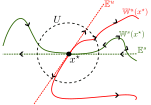
\includegraphics[width=0.6\textwidth]{global-manifolds/global-manifolds.png}
    \caption{Invariant manifolds of saddle point $x^\star$. The local stable $\mathbb{W}^s_\mathrm{loc}(x^\star)$ and unstable $\mathbb{W}^u_\mathrm{loc}(x^\star)$ manifolds of the saddle point $x^\star$ respectively can be associated with the stable $\mathbb{E}^s$ and unstable $\mathbb{E}^u$ subspaces and become tangent to them near the saddle. This follows from the Hartman-Grobman and the stable manifold theorems. The global stable $\mathbb{W}^s(x^\star)$ and unstable $\mathbb{W}^u(x^\star)$ manifolds extend the definition of the local manifolds beyond the neigborhood $U$.  Figure is inspired by Fig.~6.2.4 from Ref.~\cite{argyrisbook}.}
    \label{fig:method:invariantmanifolds}
\end{figure}

\subsection{The fate of nonlinear dynamical systems II: multistability and basins of attraction}
% Linear system are monostable: they can have only one attractor. If we now move to nonlinear systems, the situation is different. Now, trajectories can have multiple distinct fates, multiple attractors. To which attractor a trajectory goes to depends on where it starts. In a multistable system, the state space is then divided into distinct regions, wherein trajectories starting on each region go to their corresponding attractor. A simple and intuitive example is that of a ball on a certain landscape with hills and valleys. The ball of course rolls downhill and, due to friction, it eventually stops at one of the valleys.
In Sec.~\ref{method:nonlinear-I} we saw that the ultimate fate of nonlinear systems, their attractors, can be much more complicated than that of linear ones. Not only are the attractors themselves complicated, but they can also coexist in state space. If there are two coexisting attractors, this means that the state space will be separated into three regions: the basin of attraction of attractor one, the basin of attractor two, and the boundary between them. Usually, the basin boundary is formed by stable manifolds of saddle-type objects: saddle-points, saddle-limit-cycles, and even chaotic saddles! \cite{pisarchik}. Figure~\ref{fig:bistability-duffing} illustrates this for a relatively simple system with two stable equilibria, where the basin boundary is the stable manifold of the saddle-point in the middle. This system is known as the Duffing oscillator: 

\begin{align}
    &\dot{x} = v\\
    &\dot{v} = -(-kx + cv + lx^3)/m,
\end{align}

with $k = 1$, $c=0.5$, $l=1$, $m=1$. This system represents a ball of mass $m$ rolling downhill at position $x$ and velocity $v$ on a quartic potential landscape of the form $U(x) = -lx^4/4 - kx^2/2$ with a friction term $-cv$. Following the definition of global manifolds in Eq.\ref{eq:global-manifolds}, these global manifolds are essentially obtained by integrating trajectories starting on the local manifolds of the saddle-point. 
%
\begin{figure}[htb!]
    \centering 
    \includegraphics[width=0.6\columnwidth]{duffing-bistability.png}
    \caption{Bistability in Duffing model. Two stable equilibria (white square and circle) are shown with their respective basins of attraction in two shades of purple. The global stable and unstable manifolds of the saddle-point (black point) in the middle are also shown as green and red lines respectively. The global stable manifold of the saddle coincides with the boundary between the basins.}
    \label{fig:bistability-duffing}
\end{figure}


In this thesis we study two examples of multistability occuring in networked systems. In Chapter \ref{chap:malleability} we study networks of Kuramoto units, and see there the coexistence of multiple attractors depending on how strongly the units are interacting. We also see how this multistability impacts the sensitivity of the system to small changes in parameters of the units. Later, in Chapter \ref{chap:multistability} we study how multistability arises when two excitable neurons are coupled together diffusively. Both studies require that we find the attractors in the systems. This is what we deal with in the next section.

\subsection{How to find attractors}
Finding all the attractors of a given dynamical system is not necessarily a trivial task. For equilibria, one can find all the roots of the system function, i.e., $f(x^\star) = 0$ and then check their stability through the eigenvalues of the Jacobian evaluated on them. However, for more complicated attractors the problem becomes more complicated.
To start off, simply proving that a set is an attractor, following the criteria given in \secref{method:attractors-formal}, is usually not possible. Instead, in practice we use the looser definition of an attractor as the long-term dynamics of trajectories. Numerically, this means a brute-force approach of simulating several trajectories in state space for long integration times and seeing where they converge.

This comes with two problems. First, it does not rule out the possibility that a certain set is just a very long transient. To remedy this, we usually integrate trajectories on the set for very long and check if there is any escape. Second, some attractors might have very small basins of attraction, such that randomly chosen intiial conditions are unlikely to end on them, so it is unlikely that we find those attractors. So far, however, this brute force approach is the best we have for general systems \cite{}. Within this approach, there are two main methods in the literature for finding attractors. They differ in how they check converge to attractors.

The first approach was proposed in \refref{} and implemented with improvements in \refref{datseris2022effortless}. Given a trajectory, it XX.


The second approach has been proposed by \refref{gelbrecht2020monte} and soon thereafter also by \refref{stender2021bstab}. Later it was implemented efficiently with improvements in \refref{datseris2023framework}.

Both methods can be applied across a parameter range and used in a continuation fashion. Developing this method, along with implementing, improving, and maintaining the featurizing method, was one of my contributions in my PhD. This led to the publication in \refref{datseris2023framework}. The continuation method works by XX


\section{Bifurcations}
What happens to the attractors - and, in general, to the state space structures - of a dynamical system when we vary its parameters? In terms of the qualitative properties, there are two possibilties: either they stay similar or they change drastically. We can be a bit more rigorosu. Two systems are qualitatively similar if they are topologically equivalent. The notion of topological equivalence was already mentioned in \secref{method:invariant-manifolds}. As a reminder, two systems are topologically equivalent if the state space of one can be obtained by a continuous transformation of the other \cite{kusnetsov}. Mathematically, this means that they are topologically equivalent if there is a homeomorphism $h:M \to M$ mapping orbits of the first system onto orbits of the second, preserving the direction of time. 

As the parameters of a system are varied, we obtain different dynamical systems that are usually topologically equivalent. The attractors, for instance, may move, but they retain their stability. At some point, however, there may be a drastic change, and the new system may no longer be equivalent. The attractor may have disappeared, or lost its stability. Or a new attractor may have emerged. These drastic qualitative changes in the behavior of a dynamical system are called bifurcations. A bit more rigorously, a bifurcation is a change in the topological type of a system as its parameters pass through a critical (bifurcation) value \cite{kusnetsov}.
There are many different types of bifurcations, and one can literally write a whole book about this \cite{kusnetsov}. For this thesis we focus briefly on just a few bifurcations that will be relevant for later. 

\subsection{Saddle-node bifurcation (or equilibria and limit cycles)}

% In a saddle-node bifurcation two equilibria (one stable and the other unstable) coalesce and annihilate each other. Therefore, this bifurcation deals with the creation (and destruction) of stable and unstable equilibria. In this case, one equilibrium had a negative eigenvalue and the other has a positive eigenvalue before bifurcation. At the bifurcation, these values reach $0$ and later the points are destroyed \cite{strogatz_2018}. 
% This scenario also occurs for periodic orbits (e.g. limit cycles).
mention ghosts
\subsection{Hopf bifurcation}

% In an Andronov-Hopf bifurcation, a small-amplitude limit cycle is born from an equilibrium: it appears when the equilibrium disappears. In a supercritical bifurcation, the limit cycle is born stable (and the equilibrium loses its previous stability). In a subcritical, the inverse happens: the limit cycle is born unstable and the equilibrium gains stability. In this case, the Jacobian has a pair of complex eigenvalues whose real part becomes zero at the bifurcation.
\subsection{Homoclinic bifurcation}
% The homoclinic bifurcations also describe the appearance (or disappearance) of limit cycles (two-dimensional periodic orbits). The bifurcation is supercritical if the limit cycle is stable and supercritical if unstable. In the supercritical case, before the bifurcation there is a saddle and a stable limit cycle. At the bifurcation, these two touch each other, thereby making a homoclinic orbit (connecting the saddle to itself). After the bifurcation, the homoclinic orbit disappears (and the limit cycle already disappeared) and only the saddle remains. 
% In the subcritical case the behavior is similar, but the limit cycle is unstable.

 %2

\chapter{Small changes at single nodes can shift global network dynamics} \label{chap:malleability}

% \begin{center}
%     % {\Large \textbf{Small changes at single nodes can shift global network dynamic}} \\[1em]
%     {\large Kalel L. Rossi$^{1}$, Roberto C. Budzinski $^{2,3,4}$, Bruno R. R. Boaretto $^{5}$, Lyle E. Muller $^{2,3,4}$, Ulrike Feudel$^{1}$ } \\[1em]
%     {\small $^1$ Theoretical Physics/Complex Systems, ICBM, Carl von Ossietzky University of Oldenburg, Oldenburg, Lower Saxony, Germany \\ $^2$ Department of Mathematics, Western University, London, Ontario, Canada, \\ $^3$ Brain and Mind Institute, Western University, London, Ontario, Canada, \\ $^4$ Western Academy for Advanced Research, Western University, London, Ontario, Canada, \\ $^5$ Institute of Science and Technology, Federal University of São Paulo, São José dos Campos, São Paulo, Brazil}
% \end{center}


\vspace{1.5em}
\noindent
{\large\textbf{Abstract}} \vspace{0.5cm}

Understanding the sensitivity of a system's behavior with respect to parameter changes is essential for many applications. This sensitivity may be desired - for instance, in the brain, where a large repertoire of different dynamics, particularly different synchronization patterns, is crucial - or may be undesired - for instance, in power grids, where disruptions to synchronization may lead to blackouts. In this chapter \footnote[1]{This chapter is a modified form of a published manuscript: Kalel L. Rossi, Roberto C. Budzinski, Bruno R. R. Boaretto, Lyle E. Muller, and Ulrike Feudel. \textit{Physical Review Research} \textbf{5}, 013220 (2023).}, we show that networks of coupled phase oscillators with nonlinear interactions can acquire a very large and complicated sensitivity to changes made in either their units' parameters or in their connections. Even modifications made to a parameter of a single unit can radically alter the global dynamics of the network in an unpredictable manner. This occurs over a wide parameter region, around the network's transitions to phase synchronization. We argue that this is a widespread phenomenon that can be expected in real-world systems, extending even beyond networks of oscillators. 
\vspace{1.5em}



% \vspace*{\fill}  % Push the content to the bottom of the page
 


\section{Introduction}\label{sec:intro}
Several systems of practical and theoretical importance are composed of, or can be modeled as, networks of interacting units. Examples from different research areas include power grids (networks of producers and consumers of electrical energy) \cite{motter2013spontaneous}, food webs \cite{dunne2002foodweb}, networks of electronic elements \cite{crotty2010josephson}, coupled lasers \cite{nixon2011synchronized}, and neurons in the brain \cite{varela2001brainweb}. An important question is how the dynamics of single units impact the network's overall dynamics, and what happens if these units are modified. What happens to the dynamics if the units' parameters change? For instance, in ecological systems, what happens if the reproduction rate of a prey increases? In power grids, can a change in the parameters of a single generator cause a large disruption, such as a blackout? Also, what happens if the units' dynamical states are modified, e.g. by shocking the units into a different state? In the brain, how can an epileptic seizure be stopped by employing a current pulse in one particular brain region? These questions highlight the idea that a regime in which single-unit-changes can alter the whole network's behavior can be either dangerous or advantageous, and is an important topic of research which we address in this work.

In both power grids and the brain, an important phenomenon is synchronization, i.e. the coherence of frequencies or even phases of oscillations. For example, it is crucial for power grids to have their elements synchronized in the $50-60$ \SI{}{\hertz} regime \cite{witthaut2022collective}. Moreover, several functional roles have been ascribed to synchronization in the brain \cite{fries2015rhythms, varela2001brainweb, singer1999neuronal}.  For systems in which synchronization is an essential process for functioning, the question of sensitivity with respect to perturbations becomes particularly important. This has been recognized in the literature, and various types of perturbations have been considered to study the vulnerability either of the synchronized state itself or of the transition to synchronization \cite{pikovsky2001synchronization, arenas2008synchronization}.
% In both power grids and the brain, an important phenomenon is synchronization, i.e. the coherence of frequencies or even phases of oscillations. For example, it is crucial for power grids to have their elements synchronized in the \SI{50}{\hertz}-\SI{60}{\hertz} regime \cite{witthaut2022collective}. Moreover, several functional roles have been ascribed to synchronization in the brain \cite{fries2015rhythms, varela2001brainweb, singer1999neuronal}.  For systems in which synchronization is an essential process for functioning, the question of sensitivity with respect to perturbations becomes particularly important. This has been recognized in the literature, and various types of perturbations have been considered to study the vulnerability either of the synchronized state itself or of the transition to synchronization \cite{pikovsky2001synchronization, arenas2008synchronization}.

In this work, we show that systems become very sensitive to changes in parameters during transitions to synchronization, such that even changes to parameters of single units can radically alter the dynamics of the whole system.
We call this phenomenon \textit{dynamical malleability} \cite{budzinski2020synchronization}, characterized by the fluctuations in network behavior caused by changes in the units' parameters or connections. Dynamical malleability can cause problems in real-world systems in two major ways: (i) the fluctuations in the dynamics can have a large magnitude, which can lead to drastic changes in the system's spatiotemporal dynamics and (ii) fluctuations are complicated and hard to predict, so that it is unclear which units or new parameter values can keep the networks in a similar synchronization state, and which others can not. Indeed, no method available in the literature to describe phase synchronization worked satisfactorily to predict the fluctuations we observe. This clearly important issue for the design and control of systems motivates our study to analyze the mechanisms that lead to these large fluctuations. 

To address it concretely, we study networks of Kuramoto oscillators organized in ring lattices. They constitute a paradigmatic model for synchronization \cite{kuramoto1975self,acebron2005kuramoto,rodrigues2016the} and have been established as a model for real-world systems like the brain \cite{poncealvarez2015restingstate, cabral2011role, rodrigues2016the}, Josephson junctions \cite{josephson1964coupled, crotty2010josephson}, and chemical oscillators \cite{marek1975synchronization, neu1979chemical}.  The Kuramoto oscillators are phase oscillators coupled through a sine function of their phase differences. Networks with these units are well-known to have a transition from desynchronization (incoherent phases) to frequency synchronization (i.e. phase-locking, meaning constant phase differences \cite{pikovsky2001synchronization}) and to phase synchronization (small phase differences) \cite{rosenblum1996phase} as the coupling strength between units increases \cite{rodrigues2016the, acebron2005kuramoto}. 

In this work, we connect the oscillators in either of two classes of network topologies, which are of theoretical and practical importance \cite{albert2002statistical}: Watts-Strogatz \cite{watts1998collective, humphries2008network, telesford2011the} and distance-dependent \cite{rogers1996phasetransitions, rubinov2015wiring}. They have very distinct properties, but in both a change in the topology from short-range to long-range connections leads to a transition to phase synchronization in the networks \cite{hong2002synchronization, rogers1996phasetransitions}. During the transitions to phase synchronization, when the systems are only partially phase synchronized, they become dynamically malleable (i.e., sensitive to parameter changes), as illustrated in Fig. \ref{fig:sketchmalleability}. 
%
\begin{figure}[htb!]
    \centering
    \includegraphics[width=0.9\columnwidth]{figure1.png}
    \caption{\textbf{Sketch to illustrate the dynamical malleability in a typical transition to phase synchronization}. Each realization of the system's parameters leads to a different transition to synchronization, i.e. a different curve in the figure. Realizations may differ from the others, for instance, in the parameter of a single unit. We see that the transitions to synchronization are different, as both the critical value of the coupling strength and the profile of the transitions differ, with the magnitude of malleability peaking during the transitions. Fixing the coupling strength, we can also look at the distribution of the degree of phase synchronization across samples (purple inset).}
  \label{fig:sketchmalleability}
\end{figure}

Furthermore, we also show that the number of attractors of the Watts-Strogatz networks increases during their transitions to phase synchronization, meaning that these systems also become especially sensitive to perturbations made to their units' states. This goes in line with recent studies for Kuramoto oscillators with identical frequencies \cite{taylor2012there, zhang2021basins, townsend2020dense} and for Kuramoto oscillators with inertia \cite{gelbrecht2020monte}. This increased multistability acts as a dynamical mechanism that can further increase the dynamical malleability. 

Therefore, despite the wide literature and importance of synchronization, this phenomenon we describe of increased sensitivity to parameter changes, with complicated, hard-to-predict consequences to the synchronization, and which can be accompanied by multistability, has so been under-explored in the literature. Although reported sporadically in some recent works \cite{peter2018transition, taylor2016synchronization, fernandez2022emergence, budzinski2019synchronous}, it has not been the focus, and thus has not been fully explored, until now. This becomes especially relevant when we note that the behavior is widespread, extending well beyond the Kuramoto networks studied here, as supported by our observations in a variety of topologies, by similar observations in spiking \cite{budzinski2020synchronization} and bursting \cite{budzinski2019synchronous} neural networks, in cellular automata (which we exemplify in the Supplemental Material), and, importantly, by the statistical physics theory of finite-size effects on phase transitions, which we discuss later in the chapter. 

We therefore hope to demonstrate the importance of dynamical malleability, and to encourage further theoretical advancements in this area, which are needed to properly describe the wide range of behaviors and to offer tools for practical applications.  

\section{Methodology}\label{sec:methodology}

In the Kuramoto model \cite{kuramoto1975self, kuramoto1984chemical}, each oscillator is described by a phase which evolves in time according to
%
\begin{equation}
    \Dot{\theta_{i}} = \omega_{i} + \epsilon \sum\limits_{j=1}^{N} A_{ij} \sin{(\theta_{j} - \theta_{i})},
    \label{eq:main_kuramoto}
\end{equation}
%
where $\theta_{i}(t)$ is the phase of the $i$-th oscillator at time $t$, $\omega_{i}$ is its natural frequency, $\epsilon$ is the coupling strength, $N$ is the number of oscillators, and $A_{ij}$ is the $(i,j)$-th element of the adjacency matrix $\mathbf{A}$. Throughout this work, we initially draw each frequency randomly from a Gaussian distribution with mean $\mu = 0.0$ and standard deviation $\sigma = 1.0$, generating a sequence $\{\omega_{i}\}, i=1,\cdots,N$. Then, different realizations can (i) shuffle these frequencies, generating another sequence $\{\omega_{i}\}_{\mathrm{shuffled}} = \mathrm{shuffle}(\{\omega_{i}\})$; or (ii) switch the frequency of one selected unit to another value $\omega_{\mathrm{new}}$. 

The networks in this work are coupled in a ring lattice of $N=501$ units with periodic boundary conditions, and follow one of two classes of topology. 
The first class is the Watts-Strogatz (WS) \cite{watts1998collective}, which interpolates between regular and random topologies with a parameter $p$, the rewiring probability: at one extreme ($p = 0$), the topology is a $k$-nearest-neighbor lattice. From it, connections are randomly chosen according to the probability $p$ and rewired to another randomly chosen connection. In doing this, the networks have a significant decrease in the mean distance between nodes, but remain very clustered, generating small-world topologies. The other extreme ($p = 1$) is then a random topology. These networks are unweighted, so their adjacency matrix's elements are $A_{ij} = 1$ if $i$ and $j$ are connected, and $0$ otherwise.

The second class of networks follows a distance-dependent (DD) powerlaw scheme, in which any given node receives connections with weights decaying based on the distance to it. Each element of the adjacency matrix is $A_{ij} =\frac{1}{\eta(\alpha) (d_{ij})^\alpha}$, where $d_{ij}$ is the edge distance between oscillators $i$ and $j$, defined as $d_{ij} = \mathrm{min}(|i - j|, N - |i - j|)$, and $\eta(\alpha)$ is a normalization term given by: $\eta(\alpha) = \sum\limits_{j=1}^{N^\prime}\dfrac{2}{j^{\alpha}}$, such that the temporal evolution of the phases can be written as:
% 
\begin{equation}
    \Dot{\theta_{i}} = \omega_{i} + \frac{\epsilon}{\eta(\alpha)} \sum\limits_{j=1}^{N^\prime} \frac{1}{j^\alpha} \left[ \sin{(\theta_{i+j} - \theta_{i})} + \sin{(\theta_{i-j} - \theta_{i})} \right],
    \label{eq:main_kuramoto_powerlaw}
\end{equation}
where $N^\prime = \frac{N-1}{2}$ denotes half the amount of units to which $i$ is connected to (one half of the ring's length, discounting the unit $i$ itself). The equation explores the symmetry in the network to switch the summation across the network to a summation across only half, multiplied by $2$.
The powerlaw decay is thus controlled by $\alpha$, the locality parameter. For $\alpha = 0$, the network is globally coupled with equal weights between every node. As $\alpha$ increases, the weights are redistributed, so that closer units (in terms of edge-distance) have bigger weights. At the extreme of $\alpha \to \infty$, only first-neighbors are connected.

The two classes have similarities: they have topologies dominated by short-range connections at one extreme and by long-range connections at another \cite{skardal2020higher, hong2013link}. They also have differences: the first class is sparsely connected, the other densely; the first has link-disorder (different rewirings lead to different networks), the second does not.  

Integration was performed using the Tsitouras 5/4 Runge-Kutta (Tsit5) method for Watts-Strogatz networks, and an adaptive order adaptive time Adams Moulton (VCABM) method for distance-dependent networks. The integrator method was chosen for distance-dependent networks for increased simulation speed, and results were robust to different integration schemes. All methods used the DifferentialEquations.jl package \cite{rackauckas2016differential}, written in the Julia language \cite{bezanson2017julia}. Additional computational packages used were PyPlot \cite{hunter2007matplotlib} for plotting and DrWatson.jl \cite{datseris2020drwatson} for code management. The code used for simulations is accessible in the repository \cite{rossi2022github}, with the parameters used in the simulations. In particular, the control parameters we used ($\alpha$, $p$ and $\epsilon$) were generated from a uniform distribution in the range of parameters showing interesting behaviors (e.g. the transitions to synchronization), then rounded to five decimal places and used in the simulations (in the case of $p$, the distribution was uniform in the log scale). These values are reported in all figures and text, and we emphasize that no value was chosen specifically by hand: the behaviors we show in the figures are typical of the systems and can be obtained by randomly generating other values for the parameters.

We quantify the degree of phase synchronization of the network through the standard Kuramoto order parameter \cite{kuramoto1975self, kuramoto1984chemical, acebron2005kuramoto}, which is the circular average of the units' phases 
%
\begin{equation}
    r(t) = \frac{1}{N}\left|\sum\limits_{j=1}^N \exp{(i \theta_j(t))}\right|,
\end{equation} 
with $i = \sqrt{-1}$. The quantifier ranges from $0$ to $1$: if $r(t) = 1$, all the phases are the same, and the system is completely globally phase-synchronized; if $r(t) = 0$, each oscillator has a pair that is completely out-of-phase, and the system can be completely globally phase-desynchronized or in a twisted state with units having distinct but linearly spaced phases. We typically describe networks by the temporal average $R \walrus \frac{1}{T} \sum_t r(t)$  of their phase synchronization, with $T$ being the total simulation time excluding transients.
%For finite systems, this quantifier is given by $R \sim 1/\sqrt{N}$ for random phases. 


\section{Results}\label{sec:results}
\subsection{Introduction to dynamical malleability}
The networks we study here, described in Eq. (\ref{eq:main_kuramoto}), follow the basic phenomenology of transitions to synchronization in Kuramoto networks \cite{kuramoto1975self, acebron2005kuramoto}.
For very small coupling strengths $\epsilon$, the oscillators are effectively uncoupled, and the phases oscillate without any significant correlation. As this $\epsilon$ increases, the instantaneous frequencies $\dot{\theta}_i$ align first, and the units' phases become locked, but not aligned: the system becomes frequency but not phase synchronized \cite{pikovsky2001synchronization}. 

Then, whether the phases can align or not depends on the topology \cite{medvedev2014small, hong2002synchronization}. In a two-nearest neighbor lattice, where only four nearby units are connected (two on each side), there is a topological limitation in the spread of interactions across the network that makes the oscillators arrange themselves in shorter-range patterns (Fig. \ref{fig:spatiotemporal}(a)) (an exception might occur if the coupling strength is extremely high, much bigger than the relevant values studied here).
If the short-range connections are randomly rewired to long-range connections, following for instance the Watts-Strogatz (WS) algorithm, the shorter-range patterns give way to longer-range patterns, and the oscillators start to phase synchronize ((b) and (c)), until eventually a strong (though not complete) phase synchronization (PS) is reached (d). This occurs at different stages for each realization: for instance, panels (c) and (k) reach a high degree of PS, with the longer-range patterns, but panel (g) does not. 

In Fig. \ref{fig:spatiotemporal}, the natural frequencies $\{\omega_i\} (i=1,\cdots, N)$ were kept constant across panels (a)-(d). Changing the frequencies, keeping the initial conditions $\{\theta_i(0)\} (i=1,\cdots, N)$ fixed, leads to a different realization (also called sample), with possibly different dynamics. If the frequency of a single unit $\omega_i$ is changed to an arbitrary new value, for instance $\omega_\mathrm{new} = 3$, the network's behavior can be significantly altered (panels (e)-(h)). This is especially the case for networks with intermediate rewiring probabilities $p$, in which this single unit frequency change can bring the network from high to very low phase synchronization (panels (c) to (g)). The instantaneous frequencies typically remain synchronized, though their values might change. For random networks, phase synchronization is always maintained, though the instantaneous frequency values may also change. 
%
\begin{figure*}[htb!]
    \centering
    \includegraphics[width=0.99\textwidth]{figure2.png}
    \caption{\textbf{Transition to phase synchronization and the effect of a single-unit change}. The figure shows the color-coded phases $\theta$ of all oscillators in the network and the degree of phase synchronization $r(t)$ (green line) across time for Watts-Strogatz networks. The coupling strength $\epsilon$ is fixed at $\epsilon = 4.51282$ and the natural frequencies ${\omega_i}$ in the first row are the same, generated by randomly drawing from a Gaussian distribution with zero mean and unitary standard deviation. Networks in the left column are two-nearest-neighbor lattices (rewiring probability $p = 0$); the short-range connections in these networks are then rewired in the following columns, with probability $p = 0.08733$ in the second column, $p = 0.19684$ in the third, and $p = 1.0$ in the fourth (leading to random networks). Increasing the proportion of long-range connections thus leads generally to more phase-synchronized networks.
    In the second and third rows, the natural frequency $\omega_i$ of a single unit $i$ (indicated by the gray arrows) is changed to a new value $\omega_i \to \omega_\mathrm{new} = 3.0$, with all other parameters being kept fixed. The units shown in the figure were those which led to the smallest (second row) or highest (third row) degree of phase synchronization $\meanR$ out of all $N = 501$ units in the network for each value of $p$. Initial conditions were the same for all simulations, and were randomly drawn between $0$ and $2\pi$.
    }
    \label{fig:spatiotemporal}
\end{figure*}

Figure \ref{fig:spatiotemporal} thus illustrates that the long-term dynamics and phase synchronization differ in each realization. The realizations, created by changing the natural frequency of one unit, are distinct dynamical systems, so it is not surprising to observe distinct long-term dynamics. It is, however, interesting to observe how large these changes in dynamics can be, and how they depend on the topology. For instance, in networks of intermediate $p$ (second and third columns of Fig. \ref{fig:spatiotemporal}, the phase synchronization changes drastically. In random networks ($p = 1$, fourth column), they preserve the phase synchronization but alter the instantaneous frequencies of the oscillators (seen in the figure by the number of vertical lines). We also note that the behavior we describe is typical of the systems, and the values of $p$ and $\epsilon$ used here were generated as described in Section \ref{sec:methodology}. Since the fluctuations in the phase patterns (reflected in the phase synchronization) are clearer and more pronounced than the instantaneous frequency patterns, we now focus on the phase synchronization of the networks.

\subsection{Comprehensive view of dynamical malleability}
To obtain a comprehensive picture we now study an ensemble of samples obtained by shuffling the frequencies ($\{\omega_i\}_\mathrm{original} \to \{\omega_i\}_\mathrm{shuffled} = \mathrm{shuffle} \left( \{\omega_i\}_\mathrm{original} \right))$ or by changing the frequency of only a single unit to a new value ($\omega_{i, \mathrm{original}} \to \omega_\mathrm{\mathrm{new}}$). We show in Fig. \ref{fig:transition_sync} the transitions to phase synchronization with increasing coupling strength or with switching from short-range to long-range connections. As expected from Fig. \ref{fig:spatiotemporal} we also find a large dynamical malleability (sometimes simply called malleability) during the transitions. 

We study two classes of topology, Watts-Strogatz (WS, small-world) and distance-dependent (DD), described in Sec. \ref{sec:methodology}. We consider ensembles as collections of networks with fixed coupling strength $\epsilon$ and topology (fixed rewiring probability $p$ or locality parameter $\alpha$) but distinct realizations of the natural frequencies $\{\omega_i\}$ \cite{carlson2011sample}.  Each ensemble in the figure contains $501$ samples (realizations). We present the results using the mean degree of phase synchronization $R$ for each realization, and the gap $\Delta \walrus R_\mathrm{max} - R_\mathrm{min}$ between the most and least phase synchronized realizations in each ensemble. The gap $\Delta$ is chosen simply to illustrate the wide range of $R$ values clearly, and we remark that very similar curves are observed by using the standard deviation over samples.

In Fig. \ref{fig:transition_sync}, thicker lines represent an ``original" sequence of frequencies $\{\omega\}_\mathrm{original}$, from which other realizations (light lines) are created by shuffling all frequencies or changing the frequency of one unit to a new value $\omega_\mathrm{new} = 3.0$. Each sample is a different dynamical system, and has a different transition to phase synchronization, which occurs at different values of $\epsilon$, $p$, or $\alpha$, and with a different profile (some have a small region of desynchronization while others do not, for instance). 

This means that changing samples can lead to large changes in the behavior of the system, as we see throughout Fig. \ref{fig:transition_sync}. First, we study the transitions induced by increasing the coupling strength $\epsilon$ for four representative types of networks (panels (a)-(d)), characterized by four specific values of rewiring probability $p$ and locality parameter $\alpha$.

In the red curves, networks are dominated by long-range connections, with $p = 1$ (random) and $\alpha = 0$ (all-to-all)  and have a complete transition to phase synchronization (reaching $R \sim 1$), with the dynamical malleability (measured by $\Delta$) increasing during the transition and returning to zero after.
The all-to-all case is the finite-size version of the system originally studied by Kuramoto  \cite{kuramoto1984chemical}, and the critical $\epsilon$ values, when the transition occurs in each sample, are close to the $\epsilon_c = \frac{2}{g(0)\pi} = \frac{2\sqrt{2}}{\sqrt{\pi}} \approx 1.596$ predicted in the thermodynamic (infinite network size) limit. Its finite-size scaling properties and behavior have also been studied in \cite{hong2007entrainment, peter2018transition}. It is worth mentioning that this parallel between random networks and all-to-all networks, which have similar phenomenology, has been described in other works. Both have the same scaling exponents, belonging to the mean-field type \cite{skardal2020higher, hong2013link}. 

In the green curves ($p = 0.19684$ and $\alpha = 1.538463$) some connections have been rewired in the Watts-Strogatz networks, and weights redistributed for distance-dependent networks, from long-range to effectively short-range connections. On average, phase synchronization $R$ decreases, though still remaining high. Some samples of WS networks also start to display regions of desynchronization: after the initial transition to high $R$, a further increase in $\epsilon$ can desynchronize them (visible in panels (a) and (c), for $\epsilon$ roughly in $[6,7]$). Therefore, the huge changes in $R$ ($\Delta \sim 0.99$) due to changing samples can be attributed to two effects: the difference in their critical coupling strength (when the transition begins) \cite{hong2006anomalous}, and also in their different post-transition behaviors (such as the desynchronization gaps that occur at different intervals of $\epsilon$.)

In the purple curves ($p = 0.08733$ and $\alpha=1.76923$), even more short-range connections become present. Phase synchronization $R$ on average decreases, while the fluctuations $\Delta$ remain high and occur more evenly spread across samples.

Finally, for cyan curves ($p = 0$, two-nearest-neighbor chains and $\alpha = 3$, close to nearest-neighbor chains), the connections are short-range. Their phase synchronization is much smaller, and they do not reach a high degree of phase synchronization for any value $\epsilon$ we tested.
These networks with short-range connections still have some degree of malleability, but not as high as the previous two cases. 

Returning to frequency synchronization, we mention that for weak coupling strengths (roughly below $\epsilon \approx 3$), most of the samples in any ensemble are not frequency synchronized (see Fig. S3). Above this value, frequency synchronization becomes more common, especially for networks with more long-range connections, such that for sufficiently high coupling all samples become frequency synchronized. This is not the case for networks with mostly short-range connections ($p \lessapprox 0.01$), in which some samples do not reach frequency synchronization even despite strong coupling. The presence of frequency synchronization in the short-range networks is consistent with the literature \cite{strogatz1988phase, acebron2005kuramoto} showing that frequency synchronization in first-nearest-neighbor chains is possible for sufficiently high $\epsilon$ in strictly finite systems. There are therefore also sample-to-sample fluctuations in the frequency synchronization of Kuramoto networks. They occur similarly to the fluctuations in phase synchronization, but are somewhat harder to visualize and have a less interesting dependence on parameters, justifying our focus on phase synchronization in this chapter.

We now move to the topology induced transitions, which occur by switching from short-range to long-range connections (varying $p$ and $\alpha$) while keeping the coupling strength $\epsilon$ fixed (Figs. (e-h)). A similar scenario occurs with a transition to phase synchronization, induced by changing either $p$ or $\alpha$. The dynamical malleability increases during the transitions, reaching significant values for both shuffled realizations and single-unit changes. The nearest-neighbor networks show some malleability, while the long-range dominated ones (random or all-to-all) show no malleability. We note here that the transition for WS occurs at $p \sim 0.1$, so we plot the figures on logarithmic scale to show the full transition to synchronization. This transition was already reported for WS networks in \cite{hong2002synchronization}, but the authors used a linear scale for $p$ and missed the full details of the transition that we see here, especially the sample-to-sample fluctuations; for distance-dependent powerlaw networks, a transition in phase and frequency was reported in \cite{rogers1996phasetransitions}. However, none of these references studied the sample-to-sample fluctuations.

We conclude that either shuffling or changing a single unit can significantly alter the behavior of these systems, leading to a large dynamical malleability, in some cases over a very large range of parameters. This is particularly strong for WS networks, reaching $\Delta \sim 0.99$, close to the maximum possible value of $\Delta = 1.0$. The distance-dependent networks have weaker fluctuations, though still significant, reaching up to $\Delta \sim 0.7$.
%
\begin{figure*}[htb!]
    \centering
    \includegraphics[width=0.99\textwidth]{figure3.png}
    \caption{\textbf{Transitions to phase synchronization and dynamical malleability}. Networks under Watts-Strogatz (WS) and distance-dependent (DD) topologies reach phase synchronization through either an increase in coupling strength $\epsilon$ (given the topology has a sufficient amount of long-range connections) or by switching short-range connections to long-range. Fluctuations in the degree of phase synchronization $\meanR$ between samples increase during the transitions, as can be seen by the differences in the same-colored curves and by $\Delta \coloneqq \meanR_\mathrm{max} - \meanR_\mathrm{min}$. Starting from a natural frequency sequence originally drawn from a Gaussian distribution (thicker lines), the other samples (thinner lines) can be generated by shuffling the natural frequencies or by switching the natural frequency of one unit to $\omega_\mathrm{new} = 3$. For intermediate networks (purple and green curves), the increase in the fluctuations (i.e. in dynamical malleability) extends for a wide range of parameters and becomes considerably large. Each panel contains $501 = N$ realizations, with rewiring probabilities fixed for the coupling transition, with values shown in the legend, and coupling strength fixed in the topology transition at $\epsilon = 4.51282$ for WS and $\epsilon = 6.46154$ for DD. The initial conditions are the same across all realizations, and are randomly distributed from $0$ to $2\pi$. The curves of $\Delta$ are qualitatively similar with other dispersion measures, such as standard deviation, a possible difference being that the curves may be slightly shifted, as the measures can peak at slightly different values of the control parameter. We remark that the parameter values used in the simulations were generated as described in Section \ref{sec:methodology} and correspond to the typical behaviors in the system.}
    \label{fig:transition_sync}
\end{figure*}


Furthermore, we note that the networks with intermediate $p$ or $\alpha$ and the short-range networks have dynamical malleability even for high $\epsilon$. This is consistent with the known increase in the fluctuations near a phase transition \cite{ hong2007entrainment, brankov2000theory, hildebrand2007kinetic} because the networks with these parameters remain close to the topology-induced transition.
This is illustrated for WS networks in Fig. \ref{fig:Rsurface}. It shows, in the $p \text{---} \epsilon$ parameter space, the average phase synchronization across samples $\overline{\meanR}$ on the first panel and the dynamical malleability measured by $\Delta$ on the second panel. Figure \ref{fig:Rsurface} provides a comprehensive view on both the coupling strength and the topology-induced transitions. The samples are realized here as shuffles, though a similar figure would be obtained by changing one unit. There is a single region of phase synchronization for sufficiently high coupling strength $\epsilon$ and rewiring probability $p$ (panel (a)). Around the borders of this region, where the system is transitioning, the dynamical malleability is much higher (panel (b)). It then becomes clear that the intermediate networks (green and purple lines), are near the topology-induced transition (for instance, black line) for all $\epsilon \gtrapprox 1$. As $\epsilon$ increases, the networks remain near this $p$-transition, and so their dynamical malleability does not decrease. 
For the regular networks, we first note that the $p$-axis is shown on a logarithmic scale, such that these networks, with $p = 0$, are still relatively close to the transition at $p_c \approx 0.1$, and thus they also present significant malleability.

Figure \ref{fig:Rsurface} also illustrates the existence of two qualitatively different types of transitions: one induced by increasing coupling strength (for sufficiently high $p$), and another induced by increasing $p$ (for sufficiently high $\epsilon$). The difference between both is in their starting points. Both are globally phase desynchronized, but in the former (red, green, and purple lines), the weak coupling strength regimes have mostly uncorrelated oscillators, with no discernible structures in the phases or even synchronization in the frequencies. In the latter (black line), there are shorter-range structures with frequency synchronization for most samples.
%
\begin{figure*}[htb!]
    \centering
    % \includegraphics[width=1.0\textwidth]{figures/figure_1b.pdf}
    \includegraphics[width=0.99\textwidth]{figure4.png}
    \caption{\textbf{Dynamical malleability increases around the regions of transition to phase synchronization.} The surface on the left shows the average degree of phase synchronization $\overline{R}$ across the ensemble ($1000$ realizations of shuffled natural frequencies). The region of high phase synchronization is clearly seen for sufficiently high coupling strength $\epsilon$ and rewiring probability $p$. The colored lines correspond to the parameter values shown in Fig. \ref{fig:transition_sync}. The right panel displays $\Delta$, the difference between the most and least synchronized realizations for each pair $(p, \epsilon$), and we see that the fluctuations from sample to sample increase during the transitions to phase synchronization. The green and purple curves remain close to the region of transition for all $\epsilon \gtrapprox 1$, such that their fluctuations do not decrease with an increase in $\epsilon$. The figure uses Gouraud interpolation to ease visualization by smoothing the curves with a linear interpolation.}
    \label{fig:Rsurface}
\end{figure*}

\subsection{Unpredictability of dynamical malleability}
For Watts-Strogatz networks, samples can be generated by resampling the topology instead of changing the natural frequencies. Since they are generated by a random rewiring process, different realizations generate different networks (there is link-disorder \cite{hong2013link}). Therefore, different samples can also be generated by resampling the network while keeping the natural frequencies fixed. This generates a profile of dynamical malleability similar to that shown in Fig. \ref{fig:transition_sync}(e), where the network was fixed and the natural frequencies were changed (see Fig. S1 for details). 

Now, we wish to illustrate that no network, or natural frequency sequence, is alone responsible for leading to more, of less, synchronized states. Instead, the samples depend sensitively on both, especially in the region of large STS fluctuations. Figure \ref{fig:complexxsensitivity}(a) shows the degree of phase synchronization for different realizations of the networks and different shuffles of the natural frequencies, all for $\epsilon = 4.51282$ and $p = 0.08733$ with fixed initial conditions. To aid the visualization, red rectangles indicate the network with the largest $R$ for each shuffle. No network synchronizes more (or less) for any sequence of natural frequencies; and no sequence of natural frequencies synchronizes more for any network. Furthermore, if the $\epsilon$, $p$, or initial condition are changed, the whole profile of the figure also changes.
%
\begin{figure*}[htb!]
    \centering
    \includegraphics[width=0.99\textwidth]{figure5.png}
    \caption{\textbf{Fluctuations in dynamically malleable systems are unpredictable}. Panel (a) shows the average phase synchronization $\meanR$ for fixed coupling strength $\epsilon = 4.51282$ and rewiring probability $p = 0.08733$ for different $20$ shuffles of the natural frequencies $\{\omega_i\}$ and samples of networks generated by the Watts-Strogatz algorithm. For ease of visualization, the networks are ordered such that the highest network ids correspond to higher synchronization for $\mathrm{Shuffle\;id} = 1$. For each shuffle, the network with the highest $\meanR$ is marked with a red rectangle. We thus see that no network synchronizes more for all shuffles: $\meanR$ is a function of both the specific frequency and topology samples. Panel (b) shows the changes $\delta R$ in the phase synchronization $R$ when the natural frequency of each unit is changed by an amount $\delta \omega$, such that $\omega_i \to \omega_i + \delta\omega$. Other parameters are fixed, in particular $p = 0.1145$ and $\epsilon = 4.51282$. There is a rough threshold (indicated by the black dashed lines), below which changing $\omega_i$ does not significantly alter $R$ ($\delta R < 0.1$ for the figure). Furthermore, changing the frequency does not have a monotonic impact on the change in $R$: small alterations in $\omega_i$, above the threshold, can have the same impact on $R$ as bigger alterations. 
    }
    \label{fig:complexxsensitivity}
\end{figure*}
Another way to illustrate the complicated sensitivity in the region of high sample-to-sample fluctuations is by now fixing the network, and changing the frequency of a single unit by an amount $\delta \omega$. Fig. \ref{fig:complexxsensitivity}(b) illustrates the change $\delta \meanR$ in the phase synchronization, compared to the synchronization of the "original" ($\delta \omega = 0$) frequency realization. There is a rough threshold, at $| \delta \omega | \gtrapprox 0.1$, below which perturbations in one unit do not significantly affect the network's phase synchronization. Above this threshold, however, large changes occur. They are asymmetric on $\delta\omega$ and occur non-monotonically (increasing $|\delta\omega|$ does not necessarily lead to bigger changes). This complicated pattern we observe could make the design and control of these systems quite difficult in practice.

\subsection{Ratio of short to long-range connections}
As we have seen, the rewiring of connections in WS networks, or the redistribution of weights in DD networks, from short-range to long-range connections leads to a transition towards globally phase-synchronized regimes. During these transitions, the dynamical malleability peaks for some ratio of short-range to long-range connections. To quantify this ratio, we first define the short-range connections to/from a node $i$ as all existing connections to/from other nodes $j$ within an edge distance $d$ (with index $j \in [i-d, i+d]$), with $d$ being the range of short connections ($d = 2$ here). For WS networks, we calculate the average degree (number of connections) for short-range ($K_s)$ and long-range connections ($K_l$). For DD networks, we define an analogous measure of topological influence, which is:
%
\begin{align}
    K_\mathrm{s} & \walrus \frac{2}{\eta(\alpha)} \sum\limits_{j=1}^{d} \frac{1}{j^\alpha} \\
    K_\mathrm{l} & \walrus \frac{2}{\eta(\alpha)} \sum\limits_{j=d+1}^{N^\prime} \frac{1}{j^\alpha} .
\end{align}

Note that due to the symmetry of the DD networks, nodes share the same value of $K_s$ and of $K_l$. The ratio $\kappa$ of short-range to long-range connections is then defined as:
%
\begin{equation}
    \kappa \coloneqq \frac{ K_\mathrm{s} - K_\mathrm{l} }{ K_\mathrm{s} + K_\mathrm{l} },
\end{equation}
so that $\kappa = 1$ if only short-range connections exist, and $\kappa = -1$ if only long-range connections exist, with intermediate cases in between. In WS networks, the number of connections is $K = kN$ ($k$ being the amount of neighbors of each node), with the number of long connections approximately $K_l = pK$ and short-range approximately $K_s = (1-p)K$. Therefore, the ratio $\kappa$ can be easily calculated to be approximately $\kappa = 1 - 2p$. For DD networks, the ratio $\kappa$ is given as 
%
\begin{equation}
    % \kappa = \frac{ \sum_{i=1}^d \frac{1}{i^\alpha} - \sum_{i=d+1}^{N^\prime} \frac{1}{i^\alpha} }{\sum_{i=1}^N{^\prime} \frac{1}{i^{\alpha}}  }
    \kappa = \frac{ \sum_{i=1}^d i^{-\alpha} - \sum_{i=d+1}^{N^\prime} i^{-\alpha} }{\sum_{i=1}^{N^\prime} i^{-\alpha}  }.
\end{equation}


Figure \ref{fig:ratioshortlongrange} shows this ratio $\kappa$ calculated for the same setup of Fig. \ref{fig:transition_sync}(e) and (f), shuffling natural frequencies with fixed coupling strength and changing $p$ or $\alpha$. The dynamical malleability is measured here by standard deviation $\chi$ across the samples, instead of $\Delta$. The former makes the figure clearer, but the same analysis also works using $\Delta$. A remark when comparing with Fig. \ref{fig:transition_sync} is that the two measures may peak at slightly different values of $p$ or $\alpha$.  For both types of networks, the malleability peaks when there is a relatively small number of long-range connections present in a short-range-dominated network. It is more extreme for WS, as the ratios are closer to $1$ than in the DD networks. This discrepancy in the ratios leading to higher malleability shows that $\kappa$ is not an universal feature for any topology, but can still be important to understand their behavior.
%
\begin{figure*}[htb!]
    \centering
    \includegraphics[]{figure6.png}
    \caption{\textbf{Dynamical malleability peaks within a narrow interval in the relation of short-range to long-range connections}. Panel (a) illustrates the short-range (blue) and long-range (red) connections from the yellow unit for $d = 2$. Panel (b) shows the sample-to-sample fluctuations in the phase synchronization measured as the standard deviation $\chi$ of the distribution function of $\meanR$ against the ratio $\kappa$ of short-range to long-range connections calculated for several distinct topologies $p$ and $\alpha$. The green curve corresponds to the distance-dependent networks, with $\epsilon = 6.46154$ and 501 realizations per $\alpha$; purple corresponds to Watts-Strogatz networks, $\epsilon = 4.51282$ and 1501 realizations per $p$. The bottom axis show the values of $p$ and $\alpha$ for the respective ticks in $\kappa$ (note that values of $\alpha$ are not equally spaced). }
    \label{fig:ratioshortlongrange}
\end{figure*}

\subsection{Multistability}
So far, we have changed natural frequencies while keeping initial conditions fixed. Now we invert this, and shuffle initial conditions to study the system's multistability. We continue examining phase synchronization (PS) $\meanR$, although we know that $\meanR$ is only a rough measure of multistability. Being a mean value, the same $\meanR$ could represent different attractors. Therefore, the number of attractors estimated based on $\meanR$ can only be considered as a lower bound. To remedy this, we also verified the findings by comparing several other features of the dynamics. These included the standard deviation of PS in time, the PS between each unit and its neighbors, the PS between sections of $100$ units, the time-averaged instantaneous frequencies $\dot{\theta}_i$ of units, and the standard deviation, inter-quartile interval and gap between the unit's instantaneous frequencies. Realizations with unique values of all these features were considered as a distinct attractor. The number of such attractors agrees qualitatively with the dispersion we see in $\meanR$, increasing during the transition.

The phase synchronization is thus shown in Fig. \ref{fig:multistability}. Random networks ($p = 1$, red) are multistable only during their transition to phase synchronization. Intermediate networks ($p = 0.19684$, green; $p = 0.08733$, purple) have a high degree of multistability, meaning coexistence of several attractors, with very distinct degrees of phase synchronization. No shuffle of the initial conditions leads here to the same attractor, so the system has at least $501$ attractors, the number of different realizations tested.
The 2-nearest-neighbor lattice has significant multistability for $\epsilon \gtrapprox 4$. This is consistent with the literature for 1-nearest-neighbors, in which multistability occurs after the transition to phase-locking \cite{tilles2011multistable}. 
% The degree of phase synchronization $\meanR$ is also more separated in the lattices, compared to shuffling frequencies. We can see this also in the distributions, shown in Fig. \ref{fig:Rdistributions}.
%
\begin{figure}[htb!]
    \centering
    \includegraphics[width=1.0\columnwidth]{figure7.png}
    \caption{\textbf{Multistability in WS networks}. Phase synchronization and its dispersion for $501$ different shuffles (thinner lines) of the initial conditions, taken from the original initial conditions (thicker lines) used throughout the rest of this work. All other parameters are fixed, including the natural frequencies as the original frequency distribution. The coupling strength $\epsilon$ (left panel) and rewiring probabilities $p$ (right panel) are the same ones used for WS networks in Fig. \ref{fig:transition_sync}. The multistable behavior is thus very similar to what we observed before by changing the frequencies (Fig. \ref{fig:transition_sync}(a) and (e)), and so shuffling the initial conditions for this network also leads to large fluctuations in the phase synchronization. }
    \label{fig:multistability}
\end{figure}

\begin{figure}[htb!]
    \centering
    \includegraphics[width=1.0\columnwidth]{multistability-study/continuation-randomnetworks-3shuffles.png}
    \caption{\textbf{Multistability in WS networks}.}
    \label{fig:multistability-random}
\end{figure}


\begin{figure}[htb!]
    \centering
    \includegraphics[width=1.0\columnwidth]{multistability-study/continuation-smallworld-singleshuffle.png}
    \caption{\textbf{Multistability in WS networks}.}
    \label{fig:multistability-smallworld}
\end{figure}



This multistability can enhance the sensitivity of the system to parameter changes, and help to explain the large fluctuations we observe. In this case, a parameter change needs only to change the boundaries of the basins of attraction for the same initial condition to land on a completely different attractor. Attractors do not have to be necessarily drastically changed for the large dynamical malleability to be observed.
However, multistability is not in principle required for STS fluctuations; in fact, the distance-dependent networks appear to be monostable (not shown), though they are malleable. %Moreover, keeping in mind that any change of parameters or topology leads to another dynamical system, which in general possesses different attractors.

\subsection{Distributions of samples}
As we have seen, shuffling initial conditions can also generate realizations with widely different dynamics, similarly to shuffling natural frequencies. But the two methods to create an ensemble of samples have different effects, and can generate samples with distinct distributions. As shown in Fig. \ref{fig:Rdistributions} for Watts-Strogatz networks, shuffling frequencies leads usually to a broader, and smoother, distribution of $\meanR$. This increased broadness shows that new attractors are indeed created by shuffling the frequencies, so that multistability itself cannot account for the dynamical malleability we discussed previously. Furthermore, the transitions to phase synchronization occur through an increase in the distribution's average. The accompanying increase in the width of the distribution shows an increase in dynamical malleability, which goes to zero only for long-range networks ($p = 1$). 

Specifically, the distributions for the two-nearest-neighbor lattice ($p = 0$, panels (a)-(e)) are quite different: shuffling frequencies leads to a smooth distribution, whose average shifts to the right as $\epsilon$ is increased; for shuffling initial conditions there is also a slight increase in the distribution's average as $\epsilon$ is increased, but the distribution itself is dominated by several peaks. 
For intermediate networks ($p = 0.08733$ and $p = 0.19684$, panels (f)-(o)), the skewness of the distribution becomes negative, and shuffling initial conditions has a smoother behavior, more similar to shuffling frequencies. Interestingly, the distribution can be bi-modal, with the two modes being separated on either extreme of $\meanR$ (panels (n) and (o)). 
For $p = 1$ (random network), the two first coupling strengths (panels (p)-(q)) occur during the narrow interval of significant malleability, during the transition to phase synchronization. Soon after $\epsilon > \epsilon_c \approx 1.6$, the distribution becomes extremely narrow. 
%
\begin{figure*}[htb!]
    \centering
    \includegraphics[width=0.99\textwidth]{figure8.png}
    \caption{\textbf{Distributions of $\meanR$ due to shuffling frequencies or initial conditions.} Each panel contains the distribution of the mean degree of phase synchronization $\meanR$ across 20000 shuffles of natural frequencies (in purple) or initial conditions (orange) for Watts-Strogatz networks. The rewiring probabilities $p$ are indicated on the right of each row, and are the same as used in Fig. \ref{fig:transition_sync}(a); the coupling strengths $\epsilon$ are indicated on the top of each column. Bin size is $0.005$, and the probability for each bin is calculated as the occupation of the bin divided by the total occupation across all bins, and is shown in logarithmic scale.}
    \label{fig:Rdistributions}
\end{figure*}

It is worth mentioning that very similar distributions are obtained if, instead of shuffling the frequencies or initial conditions, we re-sample them from the distribution (i.e. change the seed in the random number generator).
Interestingly, the distributions are not Gaussian, which is inconsistent with the assumptions made in other works \cite{hong2007entrainment, hong2013link}. In these works, the authors argue that the fluctuations must be normally distributed for sufficiently large networks and many samples due to the central limit theorem. This inconsistency is likely generated by the finite size of the networks studied here. Even in all-to-all networks, in which there is no topological disorder, the distributions are not Gaussian for $N=501$. Results (not shown) indicate that the distributions approach Gaussian distributions as $N$ is increased to $5000$. 

\section{Discussions and conclusions}\label{sec:discussion_conclusion}
\subsection*{Summary}
In this work, we have studied the sensitivity of networks to changes in their units' parameters or connections, which we call their dynamical malleability, and showed that, near transitions to phase synchronization, this behavior acquires (i) a large magnitude, as changes to single units can radically alter the spatiotemporal dynamics, and (ii) a complicated sensitivity, as no analytical method we have tried was able to satisfactorily describe the changes to the dynamics. Parts of this behavior have been observed in isolation previously \cite{budzinski2020synchronization, taylor2016synchronization, hong2002synchronization, peter2018transition, fernandez2022emergence, budzinski2019synchronous} but this is, to the best of our knowledge, the first work to focus specifically on it and show its full phenomenology. 

To study this concretely, we have chosen ring networks of Kuramoto phase oscillators and connected the units in two distinct classes of topology, Watts-Strogatz (WS) and distance-dependent (DD). We have either changed the frequency of a single unit or changed the frequencies of all units by shuffling (i.e., redistributing) the values of the frequencies across units. The first has allowed us to verify the impact of relatively small changes, which are still not small enough to be described in the linear regime; the latter allowed us to verify the impact of redistributing the values in the network while keeping the distribution of parameters exactly the same, which is helpful for identifying mechanisms for the fluctuations. 

\subsection*{Mechanisms for dynamical malleability}
The two classes of topology we used have different characteristics (see Sec. \ref{sec:methodology}) but are similar in that they lead to networks that have two distinct types of transition to phase synchronization: one induced by increasing the coupling strength and another by increasing the dominance of long-range connections. They also have differences, mostly notably that (i) the WS networks acquire a large number of attractors during their transitions to phase synchronization (i.e. become highly multistable), while the DD networks remain with one main attractor (and possible other attractors that would have very small basins of attraction), and that (ii) the WS networks have a larger magnitude of dynamical malleability. We believe that this larger magnitude is caused by two effects: the increased number of attractors and the topology's link-disorder.

Firstly, we remark that the dynamical malleability is manifested in the networks' transitions to phase synchronization in two distinct ways. The first is through diverse onsets of the transition, as different realizations start their transitions at different values of the control parameter. This is the well-known blurriness of phase transitions described in studies of finite-size effects \cite{brankov2000theory, binder1987finite}. This effect is clearly present in both networks (see, e.g., Fig. \ref{fig:transition_sync}(a) and (b)). The second manifestation of malleability is in the post-transition fluctuations, i.e., in the sudden changes of synchronization that occur after the network has seemingly transitioned to synchronization (see, e.g. Figs. \ref{fig:transition_sync}(a) and (c)). This effect is present here mostly in the WS networks, but is also known in other systems of finite size (see, e.g. Figs. S5(b) and (d) for the case of cellular automata). It is caused at least partly by the system's multistability, as increasing the parameter can change the shape of the attractors' basins of attraction, making the same initial condition suddenly go to another attractor. So the WS networks, which have a much larger number of attractors, exhibit this additional effect that increases their malleability, while the DD networks do not.

We further remark that multistability could have an even more pronounced impact on malleability if the basins of attraction were complexly interwoven. Then, even very small changes could lead to significant fluctuations. But this does not appear to be the case in any of the networks we studied, all of which seem to have smooth basin boundaries (Fig. S4) - it is thus noteworthy that the already high dynamical malleability we have described can occur even with smooth basin boundaries. It can even occur in the absence of multistability, as seen in the DD networks.

The second mechanism for the increased malleability in WS networks is their link-disorder \cite{hong2013link}: different realizations lead to different topologies for a same parameter, and we observe a very similar phenomenology by comparing different realizations of these topologies (Fig. S1). This is a source of disorder, and thus, of fluctuations, that is not present in the DD networks. 


\subsection*{Mechanisms for the fluctuations}
As we have mentioned, the fluctuations in the malleable networks are also hard to predict. The behavior of the systems is clearly a complicated function that involves the coupling strength, topology, natural frequencies, and initial conditions all together. For instance, we have not found a sequence of frequencies, or a specific network realization, that always leads to more (or less) synchronized networks (Fig. \ref{fig:complexxsensitivity}(a)). Even for fixed frequencies and topology, the most phase synchronized realization changes depend on the initial condition or the coupling strength. Changes in the natural frequency of single units also lead to non-monotonic changes in the network's phase synchronization: the change in frequency can either increase or decrease the synchronization level, depending on the chosen unit, coupling strength, and topology (Fig. \ref{fig:complexxsensitivity}(b)).

As a consequence, we are unable to identify a specific unit, or magnitude of perturbation, that is always responsible for the greatest disruption. That is, no available theory in the literature that we have tried revealed a mechanism for the fluctuations capable of predicting them. This is a surprising result, considering the quality of the available theories, the amount of research and important advancements in the description of networks similar to the ones studied here \cite{peter2018transition, skardal2014optimal, brede2008synchrony, carareto2009optimized}. We believe that this is mainly caused by the networks' multistability, which cannot be handled by some theories, and by the wide range of synchronization patterns. 

The first theory we tried is the synchrony alignment function, which depends on the topology and natural frequencies and was shown analytically to be related to the degree of phase synchronization in the limit of strong synchrony \cite{skardal2014optimal}. It does not work satisfactorily for any dynamically malleable network that we tested. One reason for this is the weak phase synchronization in some realizations, which breaks the assumption of the method. Another, even stronger, reason is that our networks are multistable, such that the relation between the synchrony alignment function and the degree of phase synchronization given by the method cannot be satisfied for all attractors of the system. Indeed, it only worked perfectly in the strongly phase synchronized regime, which is also monostable.

The second theory we tried is due to Peter and Pikovsky \cite{peter2018transition}, who showed in all-to-all networks that different realizations of the natural frequencies synchronize differently depending on the kurtosis of the distribution. This mechanism cannot even be expected to work for the shuffling scenarios we study since they conserve the frequency distributions and thus the kurtosis as well, but we have verified that it also does not work when the units' frequencies are changed. An additional reason why this does not seem to apply in our systems may be in the topologies, which are not all-to-all.

Thirdly, we have tested other measures that have been observed in the literature to correlate to phase synchronization, and they do not work in the malleable networks. These are: (i) the proportion $p_-$ of links connecting nodes with natural frequencies of different signs \cite{brede2008synchrony};  (ii) the correlation $c_\omega$ between the oscillators' natural frequencies, taking into account the connectivity of the network \cite{brede2008synchrony, carareto2009optimized}; (iii) the correlation between natural frequencies and the node's number of connections \cite{skardal2014optimal}; and (iv) the correlation between the average frequency between neighbors of a node and the node's own frequency \cite{buzna2009synchronization, skardal2014optimal}. These results also cannot be expected to work in multistable networks, and indeed did not work in our networks. 


\subsection*{Relation to statistical physics and scaling}
As noted previously, there is a relation between our dynamical study here and studies on the statistical physics of networks. The transitions to phase synchronization that we see correspond to non-equilibrium phase transitions \cite{kuramoto1984chemical, peter2018transition}, such that we can connect the dynamical malleability we analyze with the well-known sample-to-sample (STS) fluctuations in statistical physics. These are usually described in finite systems, in which different samples have different statistical properties that lead to distinct phase transitions - the transitions are usually said to be shifted between samples \cite{sornette2006critical, hong2007finitesizescalingpre, hong2007entrainment}, which is one of the mechanisms we described for the malleability.
As seen in these studies, the size $N$ of the system (i.e. the number of nodes) influences the magnitude of the dynamical malleability as well as the interval of parameters in which it occurs. The networks we have presented in the results have $N = 501$ oscillators, and scaling analysis (Fig. S2) reveals that the intervals of high malleability decrease with the size $N$, as expected from other studies. For instance, authors in \cite{hong2007entrainment} describe the range of $\epsilon$ for high malleability as scaling with $N^{-2/5}$ for all-to-all networks. 

For the WS networks, malleability is still significant for even up $N = 5000$ oscillators. Moreover, the maximum magnitude of the fluctuations does not decrease significantly, and networks with $N = 5000$ can still reach $\Delta = 0.9$. This suggests that the malleability gets restricted to a smaller region in parameter space, but might not decrease significantly in magnitude for bigger networks. In the limit of infinite-size networks, it would get restricted to a single line, defining the two types of transitions to phase synchronization, and remain non-zero there. This is consistent with a study in all-to-all networks of Kuramoto oscillators, where this behavior was observed \cite{hong2006anomalous}. In fact, this behavior is well-known for phase transitions with quenched disorder (heterogeneous parameters), when systems are said to be non-self-averaging \cite{wiseman1995lack}.  
In any case, networks of $N = 5000$ units can be regarded as rather large in several real-world applications \cite{peter2018transition}, so the STS fluctuations we describe here occur for a significant range of system sizes.

\subsection*{Generality of the behavior}
Additionally, we show that the increase in dynamical malleability is widespread in the parameter space of the systems. Looking at this space, spanned by coupling strength and the parameter controlling the topology, the dynamical malleability remains high over a wide parameter range around the two types of transitions to phase synchronization. In particular, networks with an intermediate amount of long-range connections are highly malleable for any coupling strength $\epsilon$ we tested (e.g. green and purple lines in Fig. \ref{fig:transition_sync}). This is because the topology is fixed, so the networks remain close to the topology-induced-transition even though they are far from the coupling-strength-induced-transition. 

We also remark that the phenomenology we describe also occurs for wide ranges of topology and coupling strength values, for distinct frequency distributions, such as Cauchy-Lorenz (not shown), and for other dynamical models. For instance, previous works on spiking \cite{budzinski2020synchronization} and bursting \cite{budzinski2019synchronous} neural networks have revealed a very similar phenomenology. We also show similar behavior for cellular automata (see Fig. S5). We have observed (not shown) similar behavior in small-world networks generated by adding long-range connections and keeping the short-range ones \cite{newman1999scaling}. Other works have also observed dynamical malleability in Kuramoto oscillators coupled under both human-connectome structural networks and hierarchical-modular networks \cite{buendia2022the, villegas2014frustrated}. 
Additionally, of course, the theory of phase transitions and, consequently, of sample-to-sample fluctuations is known to apply for a variety of distinct systems. 

\subsection*{Practical importance of malleability}
The discussions lead to an interesting question: is dynamical malleability good or bad?  On the one hand, large fluctuations can be undesired. For instance, a large fluctuation could take power grids from a phase synchronized regime to a desynchronized one, and lead to blackouts. On the other hand, fluctuations can be desired due to the increased flexibility in the systems. They could be a useful mechanism for adaptation, learning or memory formation in neural circuits. More specifically, an important property of the brain is that it can separately process information from different types of input in segregated areas, and then integrate them all into a unified representation \cite{tononi1994a, tononi1998consciousness, deco2015rethinking}. For this reason, Tononi and colleagues conjectured that the brain needs to have an optimal balance between segregation and integration of areas \cite{tononi1994a}. In this optimal balance, the synchronization between different brain regions needs to fluctuate from low synchronization to high synchronization \cite{fingelkurts2006timing}. Therefore, having a large dynamical malleability can be an advantageous feature, allowing for this high variability to be achieved through small changes in the neurons, e.g. their firing rate, or their connections. There is also interesting evidence for this in \cite{li2009burst}, which reported that high-frequency firing of neurons can drive changes in the global brain state. 

\subsection*{Future research and conclusions}
An interesting line of research opened here is to understand ways to quench or to explore the fluctuations between realizations, using the framework we establish here, for practical applications. Another interesting line of research is to consider the effects of noise or time-dependent forcing on malleable systems: since they have a wider range of dynamical states available by changing parameters, a time-dependent change in the parameters, induced by the noise or forcing, can lead to transitions between several different states. The complicated and sensitive dependence on the parameters would mean that even small amplitude changes could lead to drastic fluctuations. 
For the Watts-Strogatz networks, multistability can complicate the dependence on external inputs, and make the effects dependent on the timing of perturbations, as different states, all of which coexist, can react differently to the parameter changes. Understanding these behaviors is important, for instance, in the context of neural systems, where external influences are common and where temporal fluctuations are essential.

Future research is also needed to fully describe the mechanism for the fluctuations between realizations. An interesting possibility could be to extend the synchrony alignment function \cite{skardal2014optimal} to weakly synchronized regimes or to multistable systems. Another promising approach would also be to apply the formalism introduced in \cite{muller2021algebraic,budzinski2022geometry}. A third possibility would also be to use the model reduction method by \cite{hancock2018model}. These would be important theoretical contributions for the understanding of phase synchronization in oscillator networks and for the role of each unit in a network.

To summarize, the increased magnitude and complexity of dynamical malleability shown here is a general phenomenon in finite-size systems that can be expected to occur in real-world systems. 


\section*{Acknowledgments}
We would like to thank Jan Freund and Arkady Pikovsky for helpful discussions. K.L.R. was supported by the German Academic Exchange Service (DAAD). R.C.B. and L.E.M. acknowledge the support by BrainsCAN at Western University through the Canada First Research Excellence Fund (CFREF), the NSF through a NeuroNex award (\#2015276), SPIRITS 2020 of Kyoto University, Compute Ontario (computeontario.ca), Compute Canada (computecanada.ca), and the Western Academy for Advanced Research. R.C.B gratefully acknowledges the Western Institute for Neuroscience Clinical Research Postdoctoral Fellowship. B. R. R. B. acknowledges the financial support of the São Paulo Research Foundation (FAPESP, Brazil) Grants Nos. 2018/03211-6 and 2021/09839-0. The simulations were performed at the HPC Cluster CARL, located at the University of Oldenburg (Germany) and funded by the DFG through its Major Research Instrumentation Program (INST 184/157-1 FUGG) and the Ministry of Science and Culture (MWK) of the Lower Saxony State, Germany.

 %3 chap:malleability
\chapter{Dynamical properties and mechanisms of metastability}\label{chap:metastability}


% \begin{center}
%     {\large Kalel L. Rossi$^{1}$, Roberto C. Budzinski $^{2,3,4}$, Everton S. Medeiros $^{1}$, Bruno R. R. Boaretto $^{5}$, Lyle E. Muller $^{2,3,4}$, Ulrike Feudel$^{1}$ } \\[1em]
%     {\small $^1$ Theoretical Physics/Complex Systems, ICBM, Carl von Ossietzky University of Oldenburg, Oldenburg, Lower Saxony, Germany \\ $^2$ Department of Mathematics, Western University, London, Ontario, Canada, \\ $^3$ Western Institute for Neuroscience, Western University, London, Ontario, Canada, \\ $^4$ Western Academy for Advanced Research, Western University, London, Ontario, Canada, \\ $^5$ Institute of Science and Technology, Federal University of São Paulo, São José dos Campos, São Paulo, Brazil}
% \end{center}


\vspace{1.5em}
\noindent
% \textbf{Abstract.} 
{\large\textbf{Abstract}}\vspace{0.2cm}

Metastability, characterized by a variability of regimes in time, is a ubiquitous type of neural dynamics. It has been formulated in many different ways in the neuroscience literature, however, which may cause some confusion. In this chapter \footnote[1]{This chapter is a modified form of a manuscript under review: Kalel L. Rossi, Roberto C. Budzinski, Everton S. Medeiros, Bruno R. R. Boaretto, Lyle E. Muller, and Ulrike Feudel. Dynamical properties and mechanisms of metastability: a perspective in neuroscience.} , we discuss metastability from the point of view of dynamical systems theory. We extract from the literature a very simple but general \textit{definition} through the concept of \textit{metastable regimes} as long-lived but transient epochs of activity with unique dynamical properties. This definition serves as an umbrella term that encompasses formulations from other works, and readily connects to concepts from dynamical systems theory. This allows us to examine general dynamical properties of metastable regimes, propose in a didactic manner several \textit{dynamics-based mechanisms} that generate them, and discuss a theoretical tool to characterize them quantitatively. This work leads to insights that help to address issues debated in the literature and also suggest pathways for future research.
\vspace{1.5em}

\section{Introduction}

Time-series of neural activity often reveal series of transitions between experimentally observable regimes with unique dynamical properties. For example, as subjects fall asleep, their brains progress through a series of well-defined patterns, from the 11-15 Hz sleep spindle \cite{contreras1996control}, to the large low-frequency rhythms of deep sleep \cite{steriade1993thalamocortical}, and to waking-like activity during rapid eye movement (REM) sleep \cite{jouvet1979does}. These sleep stages, or regimes, can also occur on shorter timescales, as subjects transition from passive rest to active perception \cite{poulet2008internal}. This ubiquitous phenomenon of regime switching has prompted connections to the concept of \textit{metastability} in physics and dynamical systems theory. Many works have demonstrated metastability in neural systems across different spatiotemporal scales and species \cite{michel2017eeg, vandeville2010eeg, lehmann1987eeg, jones2007natural, lacamera2019cortical, mazzucato2019expectation, recanatesi2021metastable, brinkman2022metastable, abeles1995cortical, seidemann1996simultaneously, jercog2017updown, luczak2007sequential, mazor2005transient, sasaki2007metastability, mashour2020conscious, dehaene2005ongoing, hudson2014recovery, tognoli2014metastable, popa2009constracting, curtis2015initiation, fernandez2020sleep, caruso2023single, lang2023temporal}.

Understanding the mechanisms based on dynamical systems theory that can generate such metastable regimes is crucial, especially as this knowledge can aid in the development of techniques to predict transitions between regimes and to possibly control them. The literature in neuroscience has made crucial advancements in this regard \cite{tognoli2014metastable, fingelkurts2017information, graben2019metastable, cavanna2018dynamic, brinkman2022metastable, fonollosa2015learning, deco2016metastability}, but differences in formulation between works can lead to some confusion. For instance, the explicit definition of metastability is not totally clear in the neuroscience literature (see Sec.~\ref{sec:currentformulations} for more). Further, discussions on the dynamics-based mechanisms for metastability are usually restricted to only a few possible mechanisms, depending on the context and formulation of each work.  

In this chapter, we aim to address these issues by discussing the neuroscience literature through the lens of dynamical systems theory. First, we extract from the literature a very simple but general definition of metastability, based on \textit{metastable regimes}. Regimes are epochs of a time-series identified in each work that have unique dynamical properties. They are considered metastable when they are \textit{long-lived but transient}. This idea is widespread among works not only in neuroscience, but is also similar to the well-defined view in physics and dynamical systems theory \cite{olivieri2005large, callen1991thermodynamics, yorke1979metastable}. The characterization as long-lived is specific to the system being studied, and discussed in details later. We argue that all metastable regimes share a crucial defining property in state space, which is the space spanned by all variables of a system (explained in detail in Sec.~\ref{sec:stability_and_invariance}). Simply put, metastable \textit{regimes} correspond to metastable \textit{regions} in state space, in which trajectories have a high probability of remaining inside. This idea can be formulated theoretically through the concept of almost-invariant regions \cite{froyland2005statistically, dellnitz2003congestion} (see Sec.~\ref{sec:framework} for details). 
% In this Perspective, we aim to address these issues by proposing a \textit{coherent framework for metastable dynamics} that unifies previous formulations and mechanisms from both the neuroscience and dynamical systems literatures. First, we highlight the idea of \textit{metastable regimes} that is common to observations and formulations of metastability in neuroscience. Regimes are epochs of a time-series identified in each work that have unique dynamical properties, and they are considered metastable when they are \textit{long-lived but transient}. This idea is widespread among works not only in neuroscience, but is also similar to the well-defined view in physics and dynamical systems theory \cite{olivieri2005large, callen1991thermodynamics, yorke1979metastable}. The characterization as long-lived is specific to the system being studied, and the framework we propose is flexible to this decision. We argue that all metastable regimes share a crucial defining property in state space, which is the space spanned by all variables of a system (explained in detail in Sec.~\ref{sec:stability_and_invariance}). Simply put, metastable \textit{regimes} correspond to metastable \textit{regions} in state space, in which trajectories have a high probability of remaining inside. This idea can be formulated theoretically through the concept of almost-invariant regions \cite{froyland2005statistically, dellnitz2003congestion} (see Sec.~\ref{sec:framework} for details). 

Associating metastable regimes in time to metastable regions in state space, which in turn are defined as almost-invariant \cite{froyland2005statistically, dellnitz2003congestion}, allows for a single coherent view on metastability. It also allows for a direct connection to well-known dynamics-based mechanisms from dynamical systems theory. Here, we discuss and compare several of these mechanisms in a didactic manner. By looking into them together through a general definition, we are able to add important insights into issues debated in the literature and propose new research directions to generate experimentally testable and falsifiable hypotheses about metastability in the brain, potentially including phenomena such as sleep, seizures, and computations in neural circuits.



\section{Short summary of metastability in the brain}
\subsection{Observations of metastability} \label{sec:observations}
We now review key observations that have helped to establish metastability as an important dynamical phenomenon. We focus on examples of metastability characterized by the switching between long-lived regimes of activity. These regimes are epochs of observations with unique dynamical properties identified by the authors of each work, and their characterization as long-lived depends on the specific application being considered. 
Further, as a note of terminology, these regimes are often called states in the neuroscience literature, but we avoid this here because it conflicts with already well-established terminologies in other fields of science. Instead, we believe regime is equally descriptive, and less ambiguous. In this section, we only maintain state as a synonym for regime when it refers to a well-established name, such as EEG microstates. 

Figure \ref{fig:observationsmetastability} illustrates some observations showing time-series with metastable regimes, along with two corresponding characteristics: (i) whether the transitions between the regimes occur during resting conditions (spontaneously) or if they are evoked by some stimulus; and (ii) whether the metastable regimes occur more than once in the observation (repeat) or not.  
%
\begin{figure*}[hbt]
    \centering
    \includegraphics[width=\textwidth]{observationsmetastability.png}
    \caption{\textbf{Brain activity typically evolves as a sequence of well-defined regimes that are transient but long lived.} The panels illustrate observations taken from the literature, namely EEG microstates \cite{michel2017eeg} (A), firing rate states identified via hidden-Markov-modelling (HMM) \cite{brinkman2022metastable} (B), UP and DOWN states \cite{jercog2017updown} (C), cortical wave patterns \cite{townsend2015emergence} (D), seizure-like activity \cite{wenzel2019acute} (E), and bursting in central pattern generators \cite{sakurai2016recruitment} (F). Each observation is explained in detail in the main text, and is classified into subtypes of metastability that we define in the Sec.~\ref{sec:subtypes}. }
    \label{fig:observationsmetastability}
\end{figure*}

As a first example, Fig.~\ref{fig:observationsmetastability}A shows time-series of electroencephalography (EEG) measurements performed in resting humans with eyes closed (taken from Ref.~\cite{michel2017eeg}). Colors indicate \Emph{EEG microstates}, identified from the spatial configuration of the electric potential amplitude of each electrode. These microstates remain almost constant for roughly $\SI{100}{\milli\second}$ \cite{vandeville2010eeg, lehmann1987eeg}, and then give way to other microstates.

Figures \ref{fig:observationsmetastability}B-C show results based on firing rates of neurons. In particular, Fig.~\ref{fig:observationsmetastability}B shows exemplary sequences of regimes adapted from Ref.~\cite{brinkman2022metastable}. The regimes are characterized by roughly stationary behavior in the firing rates of neurons in the gustatory cortex of rats, and are identified via the technique of \Emph{hidden Markov modelling} (HMM). Each regime lasts for roughly an order of magnitude longer than the transitions between any regime \cite{jones2007natural, lacamera2019cortical, mazzucato2019expectation, recanatesi2021metastable, brinkman2022metastable}. This is observed during both spontaneous and stimulus-evoked activity, and the sequence of such regimes is shown to encode the stimuli presented to the animals \cite{lacamera2019cortical, mazzucato2019expectation}. These regimes are proposed to serve as a ``substrate for internal computations" in the brain \cite{lacamera2019cortical}. Similar results have also been reported in the frontal cortex of monkeys during a delayed localization task \cite{abeles1995cortical, seidemann1996simultaneously}.

Figure~\ref{fig:observationsmetastability}C shows sequences of sustained firing (significant activity, \Emph{UP states}) and silence (\Emph{DOWN states}) in the firing rates of the deep layers of the somatosensory cortex of urethane-anesthetized rats (adapted from Ref.~\cite{jercog2017updown}). Each regime lasts for a significant time, with quick transitions between them \cite{jercog2017updown}. These regimes are ubiquitously observed in spontaneous activity \cite{luczak2007sequential, jercog2017updown}. 

Figure \ref{fig:observationsmetastability}D shows a sequence of complex \Emph{wave patterns} identified in the cerebral cortex of anesthetized marmoset monkeys, taken from Ref. \cite{townsend2015emergence}. Starting from local field potential data from multiple electrodes, the authors created a spatial map for the phases of the oscillations, filtered at the $\delta$ band ($1-\SI{4}{\hertz}$), from which they identified different spatiotemporal patterns, classified as plane waves (PW), synchrony (SY), node (ND), spiral (SP), and saddle (SA) \cite{townsend2015emergence}. These patterns repeat across the time series, but the probability of switching from one pattern to another differs from pattern to pattern, i.e., there is preferential switching between patterns \cite{townsend2015emergence}.
% The firing rate of neurons in slice cultures of the hippocampal CA3 region was found to evolve also as sequences of discrete, long-lasting states, separated by quick transitions \cite{sasaki2007metastability} (Fig. \ref{fig:observationsmetastability}D). The figure was taken from \cite{sasaki2007metastability} (Copyright 2007 Society for Neuroscience). Each state is identified by clustering algorithms applied to the space spanned by the principal components obtained from Principal Component Analysis (\Emph{PCA}) of the firing rates. The figure shows the raster plot of the firing, and the total activity, with colors denoting each state \cite{sasaki2007metastability}.

Mazor and Laurent \cite{mazor2005transient} (not included in the figure) measured the firing rate of neurons in the antennal lobe of locusts as the animals were presented with a variety of odor pulses. Their results suggest that, for long pulses (lasting more than $\SI{2}{\second}$), spiking activity in the antennal lobe switches between a baseline fixed point and an odor-specific fixed-point, which can last for a few seconds. Interestingly, the transition epochs between the two fixed points were found to contain the most amount of information about the stimuli, suggesting an important role for them in neural computations \cite{mazor2005transient, rabinovich2008transientdynamics}. This suggests a functional role of transitions between metastable regimes for information processing \cite{mazor2005transient, ashwin2005when}.

Figure \ref{fig:observationsmetastability}E shows the neural activity recorded by two-photon calcium imaging in mouse neocortex \cite{wenzel2019acute} (Copyright 2019 Society for Neuroscience). The neural population is being invaded by a propagating \Emph{seizure-like activity}, which appears in the middle of the time-series, and is characterized by sustained firing of a large number of neurons. Traveling as a wave, it transiently replaces the baseline regime, in which firing is more sparse and distributed. In this study, a pharmacological agent was applied to a specific region of the cortex to induce the seizure-like activity.

% Figure \ref{fig:observationsmetastability}E shows that metastable states also occur in the context of consciousness. The global neuronal workspace theory of consciousness proposes that we become conscious of a certain object (e.g. a stimulus) when the representation of that object is broadcast from local processing regions into a variety of spatially distributed regions, which form the global workspace \cite{mashour2020conscious}. This global broadcast is known as \Emph{ignition}, and is achieved through the sustained firing of the involved areas; this is shown in panel E for the local-field potential (LFP) and spikes in area D2 of the model studied in \cite{dehaene2005ongoing}. The figure is adapted from \cite{dehaene2005ongoing}. The activity of workspace neurons is thus characterized by discrete episodes of spontaneous coherent activation, with sustained firing, and quick transitions between them \cite{michel2017eeg}.


Figure \ref{fig:observationsmetastability}F shows the swim motor pattern in intracellular recordings of two neurons that belong to the swim central pattern generator of the mollusk \textit{Tritonia} \cite{sakurai2016recruitment} (adapted from Ref. \cite{sakurai2016recruitment}). These neurons respond by \Emph{bursting} when nerve PdN3 is stimulated. These bursts are phenomenologically similar to those shown later in Fig. \ref{fig:mechanismsmetastability}E (though their mechanisms might differ), and demonstrate the alternation between periods of sustained firing and periods of silence. The dynamics of central pattern generators often include metastable regimes \cite{marder2001central}. 

Another work (not included in the figure) has also found that the power spectrum of local-field potential (LFP) recordings in rats progresses as a sequence of relatively stationary regimes lasting for some time before rapidly transitioning to other regimes \cite{hudson2014recovery} (see e.g. Fig. 2 of Ref. \cite{hudson2014recovery}). This was observed as the rats recovered consciousness, when the concentration of an anesthetic was progressively decreased. The authors argue that the existence of well-defined metastable regimes is crucial for the fast recovery of consciousness \cite{hudson2014recovery}.

Additionally, we remark that several other regimes could be mentioned in this section, such as other types of seizures \cite{curtis2015initiation, babloyantz1986low}; sleep spindles \cite{fernandez2020sleep}, transient patterns of circular waves that repeatedly travel across the cortex during sleep and may aid the consolidation of memories \cite{muller2016rotating}, and the phases of local-field potentials in cats at rest \cite{tognoli2014metastable, popa2009constracting}. For further reviews on this topic, we refer the reader to Refs. \cite{tognoli2014metastable, brinkman2022metastable, cavanna2018dynamic, tsuda2009hypotheses}.

% We also note that some works mentioned previously may have not necessarily used the term metastability in their respective papers. \lm{Finally,} we note that some works interpret metastability differently than the idea of long-lasting states, and they were not included here.

\subsection{Current formulations of metastability}\label{sec:currentformulations}

% Several theoretical formulations have been discussed as a result of the observations of metastability in the brain. However, despite their large applicability, such formulations often depend on the specific context of their observations. To illustrate this issue, we depict in Figs. \ref{fig:definitionsmetastability}A-F the main formulations of metastability that we have identified in the neuroscience literature.
Several theoretical formulations have been employed to study the observations of metastability in the brain, but they have remained focused mostly on the specific context of their observations, and a general view is currently lacking. To illustrate this issue, we depict in Figs. \ref{fig:definitionsmetastability}A-F the main formulations of metastability that we have identified in the neuroscience literature.

We can generalize the formulations in Figs.~\ref{fig:definitionsmetastability}A-E as considering metastability to be a behavior with a type of variability in the dynamics. This variability can be directly observed as different \textit{patterns of activity} (Fig. \ref{fig:definitionsmetastability}A) \cite{friston1997transients, friston2000transients, varela2001brainweb, roberts2019metastable}; or \textit{patterns of synchronization} (Fig. \ref{fig:definitionsmetastability}B, where activity shifts between in-phase and out-of-phase) \cite{cabral2011role, deco2017dynamics, deco2016metastability, poncealvarez2015restingstate, aguilera2016extended}. As mentioned in the previous section, abstract regimes can be identified through techniques such as Hidden-Markov model \cite{mazzucato2015dynamics, lacamera2019cortical, brinkman2022metastable} or Principal Component Analysis (PCA) \cite{sasaki2007metastability}. Then, metastability is simply said to be the variability of these regimes (Fig. \ref{fig:definitionsmetastability}C, with each circle representing one distinct regime) \cite{mazzucato2015dynamics, lacamera2019cortical, afraimovich2010longrange, alderson2020metastable, lee2017linking, vasa2015effects, hellyer2014control, naik2017metastability, rabinovich2008transientcognitive, cavanna2018dynamic, werner2007metastability, bhowmik2013metastability}. In other works, metastability is said to occur due to variability of trajectories along different \textit{regions of state space} \cite{hudson2017metastability, graben2019metastable}; see Fig. \ref{fig:definitionsmetastability}D, where the black curve represents a trajectory passing through equilibria in colored circles, with their stable and unstable manifolds in dark green and red, respectively. For a detailed explanation of these concepts, we refer the reader to Sec.~\ref{sec:stability_and_invariance}. Metastability has also been defined as a variability along different positions on an \textit{energy landscape} (Fig. \ref{fig:definitionsmetastability}E) \cite{gili2018metastable, cavanna2018dynamic, aguilera2016extended, hudson2017metastability}. Another, more distinct, formulation of metastability is that of a behavior with \textit{integration-segregation}, in which neural assemblies transiently synchronize and desynchronize (Fig. \ref{fig:definitionsmetastability}F, where the nodes represent assemblies whose anatomical or functional connections correspond to lines, and their activity to colors, which alternate between synchronized and desynchronized) \cite{deco2015rethinking, fingelkurts2001operational, tognoli2014metastable, tognoli2014enlarging, bressler2016coordination, kelso2012multistability, hellyer2015cognitive}. 
%
\begin{figure*}[htb]
    \centering
    \includegraphics[width=\textwidth]{definitionsmetastability.png}
    \caption{\textbf{Formulations of metastability in the neuroscience literature.} A common theme among these is the presence of transitions between certain aspects of the system's dynamics (e.g., between activity patterns). The upper part of the figure (A-F) illustrates what these aspects are in each formulation, and the bottom part (G-H\supprime) shows characteristics of the transitions. Further details are available in the main text.}
    \label{fig:definitionsmetastability}
\end{figure*}

Furthermore, we remark that, while some works explicitly mention a time-scale separation in metastability \cite{hudson2017metastability, brinkman2022metastable}, others do not. 
Works also differ in regard to the possible mechanisms giving rise to metastability. Some consider that the variability in the dynamics needs to be spontaneous, occurring in autonomous systems (Fig. \ref{fig:definitionsmetastability}G) \cite{sasaki2007metastability, kelso2012multistability, roberts2019metastable, fingelkurts2008brainmind, cavanna2018dynamic}, while others argue that the variability must be externally induced, occurring in non-autonomous systems (Fig. \ref{fig:definitionsmetastability}G\supprime) \cite{jercog2017updown, hudson2017metastability}. A combination of both is also found in Refs. \cite{brinkman2022metastable, friston2000transients, lacamera2019cortical}.  
Finally, another source of difference is in the repeatability of metastable regimes: some works consider metastable regimes only when they are repeatable  (Fig. \ref{fig:definitionsmetastability}H) \cite{graben2019metastable}, while others also consider non-repeatable (Fig \ref{fig:definitionsmetastability}H\supprime) regimes \cite{brinkman2022metastable}. Examples of these types of metastability are shown in the observations in Fig. \ref{fig:observationsmetastability}.


\subsection{The common thread} \label{sec:common-thread}

As we have seen in the previous sections, the explicit formulation of metastability can vary considerably depending on context. However, there is a common thread across all the observations and formulations. It starts with the notion of regimes as epochs of a time-series with unique dynamical properties. For instance, unique spatial configurations of the EEG electric field define unique EEG microstates \cite{michel2017eeg}, and UP states have an above-threshold firing rate, while DOWN states do not \cite{jercog2017updown}. 
% The properties defining the regimes are often often stationary or almost-stationary (i.e., having constant or almost-constant statistical moments).
Further, these regimes often have constant, or almost-constant properties throughout their duration.

% Then,  even if only qualitatively, . These timescales can be, for instance, a characteristic period of the EEG oscillations, or an average firing rate of neurons. As a consequence of this long duration, the regimes are called metastable.
Then, regimes are characterized as long-lived, even if only qualitatively, establishing thus the common thread across works: \Emph{metastable regimes are long-lived but transient}. Although sometimes implicit, we believe this common thread is the fundamental aspect of metastability as a dynamical behavior. This is also the view that has been held generally in physics \cite{olivieri2005large, callen1991thermodynamics}.

In this chapter, we look into dynamics-based mechanisms that generate such metastable regimes, connecting these ideas with dynamical systems theory. To achieve this, we introduce some crucial concepts from this theory in the next section. 

% The dynamics are specified, both experimentally and theoretically, by observables (e.g., local-field potential in EEG, or neuronal firing rates). Properties can then be identified from these observables, such as wave patterns, hidden Markov states, or synchronization patterns, and they are often stationary or quasistationary in the statistical sense for the state's duration \cite{michel2017eeg, brinkman2022metastable, mazor2005transient} (as discussed in Sec. \ref{sec:observations}). 

\section{Metastability in state space}\label{sec:nonlinear}

\subsection{Stability and invariance - initial concepts}\label{sec:stability_and_invariance}

A dynamical system is a set of $N$ variables together with the rules that dictate their time evolution. These variables may be observables identified from experiments, for instance. At each instant, the values of these $N$ variables define the \textit{state} $\mathbf{s}$ of the system. The $N$-dimensional abstract space containing all possible states of a system is called the \textit{state space}. In this space, each dimension corresponds to a variable of the system. 

For example, consider a ball moving in a landscape with two wells separated by a hill (cf. Fig. \ref{fig:concepts-dynamics}A). When released, the ball rolls downhill in this landscape. Appropriate variables defining the state of the ball at any given time are its position $x$ and velocity $v$, such that we can write the state $\textbf{s}$ of the ball as a two-dimensional vector $\mathbf{s} = (x,v)$. So the state space for the ball will have two dimensions: one for $x$, another for $v$, as represented in Fig.~\ref{fig:concepts-dynamics}A\supprime. We can initialize this system by releasing the ball from a certain height with some speed, defining an initial state $\mathbf{s}_0 = (x_0, v_0)$. 

This initial state, also called initial condition, is one point in state space. Once released, that ball will evolve in time, going through a continuous sequence of different states, revolving around the well until it eventually comes to rest at the bottom of one well. This sequence of states representing the movement of the ball is called a \textit{trajectory} of the system, and corresponds to a path in state space. Equivalently, a trajectory is a set of points (a set of states). There are infinitely many trajectories in state space; one of them is represented in Fig. \ref{fig:concepts-dynamics}A\supprime as the black curve.

Dynamical systems theory shows that the time evolution of the infinitely many trajectories is governed by the properties of certain structures present in state space. It then becomes crucial to understand these structures.

To start, notice that in the example the ball eventually converges to the bottom of one of the wells because it loses energy due to friction. In general, any system characterized by energy losses will converge to \textit{attractors}, which are attracting sets of points in state space. The state of the ball at rest on the bottom of each well is an equilibrium attractor, as the trajectories converge to that state and stay on it indefinitely. The equilibrium thus does not change under the time evolution of the system, and is called \textit{invariant}. If one were to periodically kick the ball, it may start to draw a periodic motion: instead of converging to a single point, it revolves around the well and repeats its motion every certain period. In state space this corresponds to a closed loop, also an invariant set. Other invariant sets are also possible, such as chaotic sets, in which the long-term behavior of a trajectory is highly sensitive to changes in its initial conditions.

Attractors are said to be locally stable in state space: any small perturbation away from an attractor leads to a trajectory that eventually returns to it. An important remark is that this double well system has two stable equilibria, i.e. two attractors, so it is called bistable (in general, for more attractors, it would be called \textit{multistable} \cite{feudel2008complex, feudel2018multistability}). To which of the two attractors the ball converges depends on its initial state. 

Another class of important structures are unstable sets. We have one such structure in the double well: the top of the hill. If a trajectory starts exactly on top of the hill, it will stay there for an infinitely long time; again, the top of the hill is invariant. If we perturb the ball, even slightly, it will leave the top and converge to one of the wells. 

The stability of invariant sets can be understood from a geometrical point of view in state space. While the stable equilibrium attracts trajectories from all directions near it, the unstable equilibrium has specific attracting and repelling directions. In this case, the unstable equilibrium is said to be of saddle type \cite{ott2002chaos}, in reference to saddles (e.g. a horse-riding saddle), which also have such attracting and repelling directions. These directions are called the stable and unstable manifolds of the equilibrium, respectively. Figure \ref{fig:concepts-dynamics}A\supprime shows the saddle equilibrium in a red circle, with its stable and unstable manifolds as green and red curves, respectively. Saddle-points, or in general saddle invariant sets, play an important role in several deterministic mechanisms leading to metastability, as we show in Sec.~\ref{sec:mechanisms}.

Before proceeding, we remark that an alternative introduction to many of these concepts is provided in Ref.~\cite{khona2022attractor}.
%
\begin{figure*}[htb]
    \centering
    \includegraphics[width=\textwidth]{double-well-stability-metastability.png}
    \caption{\textbf{Illustration of multistability versus metastability}. Panels A and A\supprime illustrate the behavior of a ball on a double-well landscape, representing a multistable system. The stable and unstable equilibria are represented by green and red circles, respectively. In A, the ball is shown on the landscape to converge to the equilibrium on the right, where it stays indefinitely (equilibria are invariant). In A\supprime, a possible corresponding trajectory is shown in state space. The green curves leaving the unstable equilibrium denote its stable manifold, while the red curves denote the unstable manifold. In B, we suppose there is a demon kicking the ball and thus introducing white noise to its dynamics. This now makes the ball switch eternally between the two wells, and effectively transforms the previous equilibria (not invariant anymore, represented as faded circles) into metastable regions (which are almost-invariant), represented illustratively in B\supprime by the purple and green ellipses. }
    \label{fig:concepts-dynamics}
\end{figure*}


% state: $x \in M$; region of state space: $R = \{x\} \subset M$; regime: dynamical instantiation of $R$, as trajectories pass through it. invariance, stability

\subsection{Metastability and almost-invariance - definition}\label{sec:framework}
In the previous section we introduced a common notion of stability, which requires that a set is invariant, such that trajectories reaching it remain on it for infinitely long times. Now let us imagine a different scenario in the double well landscape: suppose the ball has a small demon that is constantly kicking it in randomly chosen directions with randomly chosen strengths, as illustrated in Fig.~\ref{fig:concepts-dynamics}B. This effectively adds noise to the ball´s evolution, creating a \textit{noisy} system. The landscape of course has not changed, so the \textit{noiseless} system is still the same. Therefore, the ball still tends to roll downhill, attracted towards the bottom. But the noise often kicks it away, repelling the ball from the bottom. As a result of this interplay between attracting and repelling tendencies, the ball is always in motion, revolving randomly around the bottom of one well, but never gets stuck to it. 

Eventually, by chance, the demon will give the ball successive kicks up the hill in such a way that it overcomes the top and falls onto the other well. How many kicks are needed depends, on average, on the noise strength: lower noise requires on average more kicks, such that the ball can stay around one well for very long epochs (see Ref.~ \cite{hangi1990reaction} for more details). 

So the ball with noise never converges to an attractor - instead, it moves for potentially very long times inside a region close to where the noiseless attractor is located, and eventually leaves. The noise transforms the ball´s dynamics from stable equilibria into metastable regimes, \textit{from multistability into metastability}, in the sense of long-lived but transient regimes that we discussed in Sec.~\ref{sec:common-thread} \cite{hangi1990reaction,pisarchik2014control, arecchi1985generalized, kraut1999preference, kraut2002multistability, kraut2003enhancement, feudel2008complex}. This idea is illustrated in Figs.~\ref{fig:concepts-dynamics}B and B\supprime.  It should be noted that these remarks are valid as long as the noise strengths are not large enough to create purely noisy trajectories, which just diffuse through the state space.

In the noiseless system, the bottom of each well forms an invariant set. In the noisy system, we have seen that two regions emerge in which the ball spends a long time. These regions are \textit{almost-invariant}, in the sense that trajectories inside them have a high probability of remaining inside as they evolve \cite{froyland2005statistically, dellnitz2003congestion}. An almost-invariant region $R$ can be defined such that the probability of staying inside it after some time evolution is large enough that trajectories stay inside for long periods of time. The higher the probability, the longer they stay.  These concepts have been nicely formalized in previous works \cite{froyland2005statistically, dellnitz2003congestion}, so we refer the reader to those references for more details. We provide a brief summary in the Supplementary Material.

Importantly, note that noise is, in general, not necessary for generating almost-invariant regions - as we see later in Sec.~\ref{sec:mechanisms}, there are also several mechanisms that lead to almost-invariant regions in deterministic, autonomous systems. The case with noise was used here only as a simple concrete example.

Therefore, we can say in general that a region $R$ of state space is metastable if it is almost-invariant, that is, if trajectories, once in $R$, tend to stay in $R$ for a long time before leaving. This is a key point in our work: \Emph{metastability is observed through \textit{long-lived but transient} (metastable) \textit{regimes}, and underlying any metastable regime is an \textit{almost-invariant} (metastable) \textit{region} of state space}.  

This view formalizes the notion of long-lived but transient regimes and reformulates them into properties in state space, associating a dynamical regime to its corresponding region, and associating that region to an interpretable quantity, namely the probability of trajectories remaining inside. The concept of almost-invariance is crucial for this, and serves as a theoretical tool to quantitatively characterize metastability.

In some applications, one might be concerned with the minimum duration of metastable regimes, i.e., how long regimes need to be in order to be metastable. This question requires an arbitrary decision on a threshold, which cannot be objectively decided in general; it depends on the specific application. The advantage of this definition is that it is agnostic to a minimum duration and thus flexible to this decision. Another advantage is that the decision can be made not in terms of a duration, but in terms of a probability, which may have a clearer interpretation. 

Beyond their characterization, the identification of metastable regimes is also an important problem, which has seen several solutions in the neuroscience literature, as discussed in Sec.~\ref{sec:observations}. An interesting approach is through optimization procedures that aim to maximize the probability of trajectories remaining inside the almost-invariant regions \cite{froyland2003detecting, froyland2005statistically, dellnitz2003congestion}. This can identify maximally almost-invariant regions, on which regimes will be maximally long, on average. These regions have been shown for some systems to have a particular geometrical property: they are partially separated in state space by invariant manifolds, which gives further insight into their structure and localization \cite{froyland2009almost}. 
The technical details of how this identification can be done for observed time-series, however, go beyond the scope of this work, and is the subject of ongoing research \cite{froyland2018robust}. 

Further, it is worth remarking that metastability of a regime does not fully define its dynamics. As we see in the next section, metastable regimes can be, for instance, periodic or chaotic, generated by deterministic or by noisy mechanisms, etc. A deeper analysis is required to fully characterize metastable regimes. 

%An interesting question to be investigated is how the methods previously applied in neuroscience relate to these optimization methods.


\subsection{Dynamics-based mechanisms for metastability} \label{sec:mechanisms}

The definition of metastability encompasses the observations and formulations previously reported in neuroscience. Furthermore, and crucially, it also allows one to study concrete mechanisms that generate metastable dynamics. These are known from dynamical systems theory. Some have been proposed in the context of metastability \cite{graben2019metastable, cavanna2018dynamic, brinkman2022metastable}, but others have not yet so far, to our knowledge.

Before we proceed to the mechanisms, we remark that around any metastable region there is a \textit{coexistence of attracting and repelling tendencies} \cite{tognoli2014metastable, kaneko2003chaotic}. The ability of metastable regions to retain trajectories is due to their attracting tendencies, and their finite duration is due to their repelling tendencies that push the trajectories away - for instance, in the double-well example, think of the attraction towards either of the two wells versus the repulsion due to the noise.

The double-well landscape with noise is a simple example of the general behavior of \Emph{noise in a multistable system}. As we have discussed before, trajectories spend considerable time around one well, then hop to the other well, and repeat this behavior indefinitely. This phenomenon is called \textit{attractor hopping} \cite{kraut2002multistability}: the system now has two metastable regimes, each corresponding to the dynamics around one well. In this sense, \textit{noise replaces the stable equilibria with metastable regions}. The regimes can be seen in the time-series of the ball's position $x$ in Fig. \ref{fig:mechanismsmetastability}A and the regions in the ball's state space, spanned by its position $x$ and velocity $v$, shown in Fig. \ref{fig:mechanismsmetastability}A\supprime. The times spent on each metastable region (called residence times or dwell times) follow a probability distribution, such as an exponential distribution for Gaussian white noise \cite{hanggi1986escape} (Fig. \ref{fig:mechanismsmetastability}A\textsuperscript{\everymodeprime\everymodeprime}). This mechanism of noise-induced transitions in multistable systems has been proposed for several observations of metastability in the brain \cite{brinkman2022metastable, hudson2017metastability}.

We introduced metastability with the example of a noisy system in Figs.~\ref{fig:concepts-dynamics}B-B\supprime and \ref{fig:mechanismsmetastability}A-A\ssupprime, but metastability can also occur without any noise or external input, due to several possible \textit{deterministic} mechanisms. We concentrate now on some of these, starting with a \Emph{stable heteroclinic cycle}, which is demonstrated here by a firing-rate model derived from three synaptically-coupled Hodgkin-Huxley neurons \cite{ashwin2011criteria}. Figure \ref{fig:mechanismsmetastability}B shows the time-series of a trajectory on such a cycle, performing a sequential alternation between three distinct regimes, each with a unique color. These regimes correspond to the vicinity of specific points in state space, as highlighted in Fig.~\ref{fig:mechanismsmetastability}B\supprime. They are saddle-points, like the red circle shown in Figs.~\ref{fig:concepts-dynamics}A-A\supprime, which have coexisting attracting directions (stable manifold) and repelling directions (unstable manifold). The stable manifold of one saddle is connected to the unstable manifold of the next, in what is called a heteroclinic connection \cite{ott2002chaos}. Furthermore, this cycle is stable: trajectories approach one of the saddle-points along its stable manifold and potentially spend a long time near it - then, they depart along its unstable manifold to the next saddle, and so keep cycling through them, converging ever closer to the saddles and their manifolds. This can be seen in the increasing residence times in Fig.~\ref{fig:mechanismsmetastability}B\ssupprime. Trajectories in the neighborhood of each saddle-point stay inside for considerable durations, so the neighborhood is a metastable region (even though the saddle-point itself is invariant and unstable).

Importantly, it can be shown that such heteroclinic cycles can globally attract trajectories \cite{nowotny2007dynamical} and are also conserved under small parameter changes (they are structurally stable) \cite{rabinovich2008transientcognitive}.  Moreover, it has been shown in neural networks that heteroclinic cycles depend on the inputs to the neurons, such that the cycle is sensitive to the stimulus to the network \cite{rabinovich2001dynamical}. Once the stimulus is applied, and the cycle is defined, it is robust against noise. So this mechanism can allow for robustness to noise while keeping sensitivity to inputs \cite{rabinovich2001dynamical, rabinovich2008transientcognitive}. This, on top of the cyclic behavior, means that heteroclinic cycles are important structures to perform sequential \textit{computations} \cite{fonollosa2015learning}.
% An example of this is for chunking dynamics, whereby information to be stored in memory is represented a phone number, e.g. $858-535-22-30$, is separated into $4$ chunks: $848$, $535$, $22$, and $30$. Trajectories representing this number cycle through the chunks as $848 \to 535 \to 22 \to 30$. Each chunk by itself is composed of sequences of saddle points representing the digits, e.g. $8 \to 5 \to 8$. In this way, sequential memories can be encoded by heteroclinic cycles of heteroclinic cycles of saddle points \cite{fonollosa2015learning}}. 
An example of this is chunking dynamics, in which a trajectory coding for a memory alternates along a heteroclinic cycle composed of further heteroclinic cycles, each corresponding to chunks of a memory \cite{fonollosa2015learning}. As such, stable heteroclinic cycles have also been proposed as the mechanism behind experimental observations \cite{rabinovich2008transientcognitive, rabinovich2008transientdynamics, rabinovich2012information} and theoretically hypothesized as a mechanism for cognition \cite{fonollosa2015learning, rabinovich2014chunking}. Heteroclinic cycles can be extended to heteroclinic networks; for a review, see \cite{hildegard2023heteroclinic}. 
%
\begin{figure*}[hbt]
    \centering
    \includegraphics[width=\textwidth]{mechanismsmetastability.png}
    \caption{\textbf{Dynamics-based mechanisms of metastability.} Each column corresponds to a distinct mechanism. The first row (A-E) shows a representative time-series, with alternations between metastable regimes, each receiving a distinct color. The second row (A\supprime-E\supprime) shows the state space of each system with the trajectory corresponding to the time-series above. The third row (A\ssupprime-E\ssupprime) shows the distribution of residence times in each metastable region for several trajectories. Further details are discussed in the main text and Supplemental Material.}
    \label{fig:mechanismsmetastability}
\end{figure*}

% Now we move to another example, which involves a \textit{chaotic attractor} that originates from an \textbf{attractor-merging crisis}. \kl{In this case, the chaotic attractor can be decomposed into two distinct sub-regions, each of which acts almost like a separate chaotic attractor: trajectories spend on average a long time on one sub-region before switching to another sub-region, repeating this process indefinitely. Figures \ref{fig:mechanismsmetastability}C-C\supprime illustrate this intermittency in a time-series and state space, respectively, with the metastable regimes or regions colored green and purple. The transitions between the regions are mediated by a particular periodic trajectory of type saddle (having stable and unstable manifolds), which therefore acts as the gateway between the regions - trajectories on one sub-region approach it and are taken to the other sub-region. It thus acts as the repelling tendency mediating the transitions between the sub-regions. Geometrically, the attractor-merging crisis occurs through a parameter change that causes two separate chaotic attractors to collide with a saddle periodic orbit, and become connected in a single, larger, chaotic attractor}.
Now we move to another example, which involves a \textit{chaotic attractor} that originates from an \textbf{attractor-merging crisis} \cite{grebogi1987critical}. In this case, the chaotic attractor can be decomposed into two distinct sub-regions. For a different parameter value of the system, these sub-regions are separate chaotic attractors. Starting from some critical parameter value, they merge together into a combined chaotic attractor, with a specific pathway connecting them. Then, trajectories in each sub-region oscillate chaotically for a long time, on average, before they switch to the other sub-region, and repeat this process indefinitely. Figures \ref{fig:mechanismsmetastability}C-C\supprime illustrate these two intermittent regimes in a time-series and their corresponding regions in state space, respectively, colored green and purple in both. The specific pathway guiding the transitions between each sub-region is a particular periodic trajectory of type saddle (having stable and unstable manifolds) - trajectories on one sub-region approach this trajectory and then are taken to the other sub-region. It thus acts as the repelling tendency mediating the transitions between the sub-regions.
The probability distribution of residence times on each of these metastable regions is exponential (Fig. \ref{fig:mechanismsmetastability}C\ssupprime). 

It is interesting to note that the trajectories for this mechanism look similar to those for the noisy bistable systems (compare Figs. \ref{fig:mechanismsmetastability}A and \ref{fig:mechanismsmetastability}C). The key difference is that the transitions in the former are caused by noise, and in the latter they are caused purely by the deterministic dynamics of the system on the attractor, with the mediating saddle periodic trajectory. Still, this highlights the often apparent similarity between noisy and chaotic dynamics, and the need for deeper analysis to distinguish between both \cite{boaretto2021discriminating}. 

Similar dynamics occur as a result of another mechanism, an \textbf{interior crisis} \cite{grebogi1983crises, ott2002chaos}. Also in this case, trajectories intermittently switch between two sub-regions of the same chaotic attractor. But the underlying structures are different from the attractor-merging crisis: a change of parameters causes a chaotic attractor to connect to a chaotic set that is unstable (a chaotic saddle, which we see more in Fig. \ref{fig:mechanismsmetastability}E-E\ssupprime). This connected chaotic attractor now includes both regions, but trajectories stay inside each sub-region for long times, before switching to the other. These transitions are again mediated by a special pathway, a periodic trajectory of saddle type, which acts as the repelling tendency. The distribution of times on the region occupied by the original chaotic attractor is again exponential. See Ref.~\cite{ott2002chaos} for more details.

Another example of a chaotic attractor that can be decomposed into two metastable regions occurs in \Emph{type-I intermittency}. We show in Fig.~\ref{fig:mechanismsmetastability}D an example in a 3-dimensional system. The trajectory alternates between metastable regimes: one with clear chaotic dynamics (in purple) and another with seemingly periodic dynamics (green). Looking at the state space in Fig.~\ref{fig:mechanismsmetastability}D\supprime, we note that the purple regime corresponds to a region that looks clearly chaotic (fractal-like structure), while the green regime corresponds to a region that looks like a periodic orbit (a closed loop). Trajectories can spend a considerable amount of time on the green region, looking periodic. When they leave it, they can then spend a long time in the purple region, leaving it when they approach the green region again.
Mechanistically, the green region is actually the \textit{ghost} of a stable periodic orbit that exists for different parameter values \cite{pomeau1979intermittency, pomeau1980intermittent, strogatz2002nonlinear}. That stable periodic orbit is destroyed by a collision with an unstable periodic orbit at some critical parameter value, leaving behind only the ghost, which is not an invariant structure \cite{medeiros2016trapping}. The bifurcation giving rise to this behavior is a \textit{saddle-node bifurcation of periodic orbits}. It can also occur analogously for equilibria, and we refer the reader to Refs.~\cite{koch2023beyond, sussillo2013opening} for further work and illustrations. Importantly, the two metastable regions in our example belong to the same chaotic attractor, and the trajectories near the ghost merely \textit{appear} to be periodic. 
Further, the time spent near the ghost can be considerably long, but is finite for any fixed parameter \cite{pomeau1980intermittent} (see the distribution of times in Fig. \ref{fig:mechanismsmetastability}D\ssupprime).

The type-I intermittency mechanism, along with the two crises discussed before, are three of many concrete instances of an idea proposed by Friston \cite{friston2000transients}, who argues that different metastable regimes can correspond to different sub-regions of a same invariant set (usually attracting). 

An important remark is that this mechanism does not require a chaotic attractor, as it occurs whenever a saddle-node bifurcation is nearby in parameter space. The chaotic attractor in the example only acts to re-inject the trajectories that leave the neighborhood of the ghost back onto it, creating a repeatable metastability. This re-injection can also occur due to noise, not only chaos \cite{medeiros2016trapping}. But if there is no re-injection mechanism, nearby trajectories will pass the neighborhood of the ghost only once, and then this is an example of non-repeatable metastability.

This saddle-node mechanism has been proposed by Kelso and colleagues as a mechanism for metastability in the brain \cite{kelso1991an, tognoli2014metastable}. Ghost structures have also been shown to play a role in the dynamics of recurrent neural networks performing particular computations \cite{sussillo2013opening}. Further, similarly to the idea of cycles of saddle-points (Figs. \ref{fig:mechanismsmetastability}B-B\ssupprime), cycles of ghost structures can also be constructed, and have been shown to generate sequences of metastable regimes that are robust in the presence of noise, having potential advantages over cycles of saddle-points \cite{koch2023beyond}. 

% It is another example of the general proposal by Friston \cite{friston2000transients}, since the trajectories here live on a chaotic attractor, which can nevertheless be separated in two distinct dynamical regimes: nearly-periodic (green) and chaotic dynamics (purple). 

Another mechanism that leads to metastable regimes is due to a \Emph{chaotic saddle}. A chaotic saddle is similar to a chaotic attractor, with the distinction that it also has repelling directions - it is thus the analogue of a saddle equilibrium for a chaotic set \cite{lai2009transient}. As a consequence, trajectories can stay near the chaotic saddle for potentially very long times, displaying chaotic dynamics, but are eventually expelled from it \cite{yorke1979metastable}. Figure \ref{fig:mechanismsmetastability}E shows a trajectory switching from a regime near a chaotic saddle (in purple) to one on an equilibrium (in green); the corresponding regions in state space are shown in Fig. \ref{fig:mechanismsmetastability}E\supprime. Note that the trajectories leave the chaotic saddle because they are not on it exactly; they are only near it. These are the typical trajectories, which are the ones numerically and experimentally observed. They form a metastable region even though the chaotic saddle itself is invariant and unstable. Ultimately, the trajectories converge to the stable equilibrium and remain on it infinitely long.
The residence times for different initial conditions near the chaotic saddle follow an exponential distribution \cite{grebogi1983crises} (Fig.~\ref{fig:mechanismsmetastability}E\ssupprime).
% We remark that trajectories on the chaotic saddle resemble the ignition behavior leading to conscious access shown in Ref. \cite{dehaene2005ongoing}.

A chaotic saddle has been reported in networks of spiking neurons \cite{ansmann2016selfinduced}, in which, interestingly, it can be subdivided into three distinct dynamical regimes, corresponding to three distinct sub-regions, which are all intermittently visited for considerable durations. Therefore, also every sub-region of that chaotic saddle can be considered metastable. That is thus an example of \textit{hierarchical metastability}, in which metastable regions contain inside more metastable regions, and the dynamics progresses through a hierarchy of metastable regimes \cite{cavanna2018dynamic}. Chaotic saddles have also been observed in other networks of spiking neurons \cite{keplinger2014transient, lafranceschina2015impact, hartle2017transient, kaminker2019alternating}, and may play a key role in synchronization processes \cite{medeiros2018boundaries, medeiros2019state}.

There are several other dynamics-based mechanisms for metastability beyond the ones discussed previously. One example is \Emph{on-off intermittency}, which is common, for instance in systems that can completely synchronize \cite{ashwin1994bubbling, ott1994blowout}, and occurs during transitions from synchronization to desynchronization induced by changing the coupling strength between units. During these transitions, systems with on-off intermittency have trajectories that intermittently switch from a synchronized regime to a desynchronized one and back. The mechanism for this intermittency, and its statistical scaling, has been studied in detail \cite{ platt1993onoff, heagy1994characterization, hammer1994experimental, cenis1997symmetry}. It is one out of many possible mechanisms that can realize the coexistence of integration (synchronization) and segregation (desynchronization), often mentioned as a crucial need for the brain \cite{fingelkurts2001operational, tognoli2014metastable, tognoli2014enlarging, deco2015rethinking}. It is also a possible mechanism for the intermittent switching between UP and DOWN states exemplified in Fig. \ref{fig:observationsmetastability}C. Furthermore, evidence for on-off intermittency has been reported for EEG data of non-convulsive paroxysmal (high-amplitude) activity in rats with genetic absence epilepsy \cite{hramov2006onoff}. The study identified a power-law distribution of residence times characteristic of on-off intermittency in regular brain activity, which alternated with the epileptic paroxysms.
A very similar mechanism is in-out intermittency \cite{ashwin1999transverse, ashwin2001influence,saha2018characteristics, saha2017extreme}. In addition, evidence for yet another type of intermittency, known as type-III intermittency \cite{pomeau1979intermittency}, has been reported in \cite{velazquez1999type}.

Metastability can also manifest as \Emph{mixed-mode oscillations}, in which trajectories alternate between regimes of small and large amplitude oscillations \cite{desroches2012mixed}. There are various mechanisms for mixed-mode oscillations, which can involve forcing the system to induce changes in parameters or through an adaptation variable that enables the switching between the two modes \cite{desroches2012mixed, rotstein2014mixedmode}. 
A particular example of mixed-mode oscillations is \emph{bursting} behavior occurring in neurons, characterized by quick firing of spikes followed by a quiescent period (as in Fig. \ref{fig:observationsmetastability}F). Bursting is a ubiquitous mode of firing in neurons \cite{fox2015bursting}, and can have important functional roles due to its ability to generate more robust responses \cite{swadlow2001impact}. A simple model displaying bursting is the Hindmarsh-Rose neuron \cite{hindmarshmodel1984}. In it, an adaptation current causes the switching between the tonic spiking and the silence \cite{hindmarshmodel1984}. The whole trajectory is on a stable limit cycle, but can still be decomposed into the tonic spiking and the silence, each of which can be considered metastable. This is yet another example of the idea proposed by Friston in \cite{friston2000transients}. Beyond this model, bursting behavior occurs in systems with a period-adding cascade \cite{kartanak2014route}.  
Mixed-mode oscillations can also occur as neuronal avalanches, which are cascades of activity occurring in varying sizes and durations, and across different scales, seen in local-field potential activity \cite{beggs2003neuronal}. An example of a dynamics-based mechanism generating avalanches has been recently elucidated in \cite{contreras2023scale}. The onset of these avalanches may be associated with critical phenomena in the brain (see Ref. \cite{girardi2021brain} for a recent review).

% Furthermore, in neuronal networks, spontaneous local field potential activity cascades across various scales within the system, giving rise to neuronal avalanches of varying sizes and durations \cite{beggs2003neuronal}, providing another example of metastability. An example of a dynamical mechanism generating avalanches has been recently elucidated in \cite{contreras2023scale}. As a branching process, the onset of these avalanches may be associated with critical phenomena in the brain (see Ref. \cite{girardi2021brain} for a recent review).}

% A similar important behavior is \Emph{mixed-mode oscillations}, in which trajectories alternate between periods of small amplitude (e.g., sub-threshold) and large amplitude oscillations (e.g., spikes) \cite{rotstein2014mixedmode}. There are various mechanisms for mixed-mode oscillations, which can involve either forcing the system to induce changes of parameters or through an adaptation variable that enables the switching between the two modes \cite{desroches2012mixed, rotstein2014mixedmode}.

Moreover, an important example of metastable behavior is \Emph{chaotic itinerancy} \cite{kaneko2003chaotic}. This phenomenon has also been discussed in the context of neuroscience \cite{freeman2003evidence, tsuda2009hypotheses, tsuda2015chaotic}, and can include several specific mechanisms, and thus is also an umbrella term, but more specific than metastability as we define it here.



\subsection{Subtypes of metastability} \label{sec:subtypes}
The definition of metastability proposed in Sec.~\ref{sec:framework} acts as an umbrella term encompassing several distinct observations, formulations, and mechanisms. More specific formulations, which restrict the phenomenon to particular contexts, can be defined as subtypes of metastability. 

As a first example, we may think of \Emph{spontaneous and driven} metastability (illustrated in Figs.~\ref{fig:definitionsmetastability}G-G\supprime respectively). They differ in regards to how transitions between metastable states are generated. In \textit{spontaneous} metastability, the mechanism behind transition is intrinsic to the system, and thus occurs without the need of external perturbations - such as noise, or stimuli. This is the case for Figs. \ref{fig:mechanismsmetastability}B-E\ssupprime. Driven metastability is the opposite: transitions occur because of external perturbations, as in Fig. \ref{fig:mechanismsmetastability}A-A\ssupprime. Each subtype has distinct but important functional roles: spontaneous metastability enables transitions between regimes without the expenditure of additional energy to stimulate the transitions \cite{tognoli2014metastable}, and guarantees that a system does not get stuck in the same regime \cite{ito2008dynamics}; driven metastability is important for direct control of the transitions, such as in stimulus-evoked scenarios.

A second important pair of subtypes is \Emph{repeatable versus non-repeatable metastability} (Figs. \ref{fig:definitionsmetastability}H-H\supprime). These are characterized by whether the metastable regimes eventually repeat in the time series or not. If the metastable regimes repeat along observations, the metastability is repeatable; if they do not, it is non-repeatable. The case of non-repeatable regimes is sometimes called metastability en route to ground state \cite{brinkman2022metastable}. Note that the observations in Fig. \ref{fig:observationsmetastability} and the mechanisms in Fig. \ref{fig:mechanismsmetastability} are already classified into these subtypes. 


\section{Conclusions and outlook}
In this chapter we have provided a discussion on metastable brain dynamics in a way that is consistent across observations and theory in both neuroscience and dynamical systems. With this, we have looked into several dynamics-based mechanisms that generate metastability, and compared them to obtain insights into their commonalities, distinctions, and connections to previous literature.

The first step was to extract a general definition of metastability from the literature: metastable regimes are long-lived but transient. This serves as an umbrella term encompassing the other formulations in the literature, is useful to interpret observations, and readily connects to dynamical systems theory. We then looked deeper into how these metastable regimes behave in state space. To achieve this, we introduced the notion of almost-invariant regions of state space, characterized by a high probability (smaller than one) that trajectories, once inside them, remain inside \cite{froyland2005statistically, dellnitz2003congestion}. Trajectories can enter an almost-invariant region, stay inside for a long time, and eventually leave. While inside such a region, trajectories exhibit time-series containing long-lived but transient epochs with unique dynamical properties, i.e. metastable regimes. The dynamics of the regimes corresponds to the dynamics in the regions (e.g., periodic or chaotic). Thus, almost-invariant regions, which we identify as metastable regions, underlie the dynamics of metastable regimes. 

With this view, we have then discussed the \textit{dynamics-based mechanisms} for metastability, i.e. how metastable regions and regimes are generated, and how they behave. Dynamical systems theory provides several concrete possibilities. Some of these have been previously discussed in the neuroscientific context \cite{graben2019metastable, cavanna2018dynamic, brinkman2022metastable}, but some are also new, to the best of our knowledge. Though not a comprehensive list, we believe it serves as a good starting point for researchers both in neuroscience and dynamical systems intending to study metastability. 

Looking at so many different mechanisms together provides several insights. To start, it provides concrete examples of metastable regimes corresponding to trajectories visiting metastable (almost-invariant) regions. Further, it becomes clear that around each metastable region there is a \textit{coexistence of attracting and repelling tendencies in state space}, as has been discussed in Refs. \cite{tognoli2014metastable, kaneko2003chaotic}. These realizations further validate the definition, which is general but still meaningful to allow for common underlying principles.

With this rich list of possible mechanisms, we have been able to provide several concrete instances of an idea that was abstractly proposed by Friston in Ref.~\cite{friston2000transients}: that the same attractor can have multiple sub-regions, each corresponding to one metastable regime. An interesting instance of this has been reported in Ref.~\cite{ansmann2016selfinduced}, in which networks of spiking neurons display a chaotic saddle (its neighborhood a metastable region) that can be further subdivided into three sub-regions, each metastable and corresponding to different patterns of activity. 

We have also suggested more dynamics-based mechanisms that can account for the important behavior of coexistence of segregation and integration: besides the important saddle-node bifurcation of fixed points that often occurs \cite{tognoli2014metastable}, we also mention in-out and on-off intermittency as mechanisms that lead to variability of synchronization \cite{ashwin1994bubbling, saha2018characteristics}. 

The solid theoretical background offered by the idea of almost-invariant regions allows us to provide objective answers to issues debated in the literature. The distinction between attractors and metastable regions, and hence between \textit{multistability and metastability} becomes clear. As discussed in Sections~\ref{sec:stability_and_invariance} and \ref{sec:framework}, attractors are invariant: trajectories on them remain on them infinitely long; meanwhile, metastable regions are only almost-invariant: trajectories eventually leave them. 
A system is called multistable when it has multiple coexisting attractors for fixed parameters, a typical behavior in nonlinear dynamical systems \cite{feudel2008complex, feudel2018multistability}. In a multistable system, trajectories converge to one of the attractors, selected by their initial conditions, and remain on this attractor forever. There are no transitions between attractors in a multistable system. If external perturbations such as noise are introduced to a multistable system, the trajectories do not stick to attractors anymore, but can hop between them \cite{hangi1990reaction}. In this case, multistability is \textit{substituted} by metastability \cite{pisarchik2014control}. An important remark is that, when the noise is too strong, it can overpower any dynamics of the system and then there is neither multistability nor metastability observable, only a random motion \cite{kraut2002multistability}.
Crucially, however, stability (and multistability) can \textit{co-occur} with metastability in autonomous systems, without noise. For instance, an attractor can be in some cases decomposed into two or more metastable regions, as discussed previously and in Sec.~\ref{sec:mechanisms}. Then, trajectories remain eternally inside an attractor, but with transitions between its metastable regions.  
% If a system has multiple attractors for fixed parameters, a typical behavior in nonlinear dynamical systems, it is multistable \cite{feudel2008complex, feudel2018multistability}. In a multistable system, trajectories converge to one of the attractors, selected by their initial conditions, and remain on the attractor forever. There are no transitions between attractors in a multistable system. If external perturbations such as noise are introduced to a multistable system, the attractors cease to be invariant regions. If the noise is not too strong, the attractors are substituted by metastable regions, and trajectories can hop between these regions. If the noise is too strong, no patterns are seen \cite{kraut2002multistability}, and there is neither multistability nor metastability observable, only a random motion. 
% In the case of sufficiently weak noise in a multistable system, the multistability is \textit{substituted} by metastability. However, in other circumstances, without noise, stability (and multistability) can \textit{co-occur} with metastability. For instance, an attractor can be in some cases decomposed into two or more metastable regions, as discussed previously and in Sec.~\ref{sec:mechanisms}. Then, trajectories remain eternally inside an attractor, but with transitions between its metastable regions.  

Another point that is often debated is whether both \textit{spontaneous and noise-induced} cases should be considered as metastable \cite{kelso2012multistability, cavanna2018dynamic, hudson2017metastability}. Here, we provide an objective answer: since there are almost-invariant regions underlying the dynamics in both cases, both are metastable. This is exemplified through the motion in the double-well landscape with noise (Figs.~\ref{fig:mechanismsmetastability}A-A\ssupprime) and the intermittency due to an attractor-merging crisis (Figs.~\ref{fig:mechanismsmetastability}C-C\ssupprime), in which also the phenomenology in the time-series, in state space, and in the distribution of residence times is strikingly similar. This means that many dynamics-based mechanisms may underlie the same observation. Therefore, the characterization of regimes as metastable is only part of the story: they possess other dynamical properties that also need to be studied. Developing methods to achieve this and properly distinguish between various mechanisms is still a subject of future research.

Understanding dynamics-based mechanisms is an important first step for \textit{predicting} transitions between metastable regimes. This is particularly important in the context of seizure prediction, an area that has deservedly received a lot of attention but which still has many open questions \cite{kuhlmann2018seizure}. Knowledge of the dynamics-based mechanism underlying transitions from normal brain activity to seizures has been recognized as a key development in the field \cite{kuhlmann2018seizure}, but that alone may not be enough: part of the difficulty may be the co-existence of several mechanisms, not just one. A more comprehensive understanding of the mechanisms for metastability, extending the ideas proposed here, could prove useful to address these difficulties through a better understanding of the precursor dynamics of transitions \cite{rings2019traceability}. A possible future path can also aim to determine mechanisms underlying observations through the use of techniques to identify system equations from data \cite{voss2004nonlinear, brunton2016discovering, tabar2019analysis, anvari2016disentangling, jacobs2023hypersindy}. 
% \kl{Understanding dynamics-based mechanisms is an important first step for \textit{predicting} transitions between metastable regimes. This is particularly important in the context of seizure prediction, an area that has deservedly received a lot of attention but which still has many open questions \cite{kuhlmann2018seizure}. There, knowledge of the dynamics-based mechanism underlying seizures would be of great use \cite{kuhlmann2018seizure}, but may not be enough. Part of the difficulty may be the co-existence of several mechanisms, not just one, and also that some mechanisms may not even have clear early-warning signals \cite{boettiger2013early, wilkat2019no}. A more comprehensive understanding of the mechanisms for metastability, extending the framework proposed here, could prove useful to address these difficulties through a better understanding of early-warning signals or of precursor dynamics behind transitions \cite{rings2019traceability}. A possible future path can also look to determine mechanisms in observations through the use of techniques to identify system equations from data \cite{voss2004nonlinear, brunton2016discovering, tabar2019analysis, anvari2016disentangling, jacobs2023hypersindy}.} 


% Further, important questions that arise when looking at these mechanisms together are: how can the transitions between metastable regions be predicted? are there early-warning signs for transitions? are there specific pathways in state space through which transitions happen, which could then be explored to define predictors?  These are understood for some mechanisms (WHICH?), but not all, and thus constitute an important avenue of future that can leverage this framework to compare the mechanisms. These questions are particularly important in the context of seizure prediction, an area that received a lot of attention, but which has still not been solved \cite{}. Knowledge of the dynamical mechanism underlying seizures would be of great use \cite{lehmann}, and recent advancements in the identification of system equations from data \cite{voss2004nonlinear, brunton2016discovering, tabar2019analysis, anvari2016disentangling} could prove very fruitful here this regard. However, we hypothesize that part of the difficulty in predicting seizures may be the coexistence of several mechanisms, such as the ones shown here, at play behind the transitions to and out of seizures. Further, at least some of these mechanisms might not have well-known early-warning signs, or might not have them at all. We propose that a complementary approach would be to extend the framework here: understand eventual early-warning signs for several metastability mechanisms to guide the development of predictors, and then apply these to real time series. In this sense, to leverage the theory to guide the development of techniques.

% A related question is: how can long-lasting metastable states be distinguished from stable states? (see e.g. Ref. \cite{wang202150}). Future works can complement our framework to probe this question, as each dynamical mechanism has distinctive signatures that can be explored to identify them from experimental data. Knowledge of the mechanisms is crucial for developing better control techniques and for better predicting their behavior. This possibility constitutes an exciting avenue of future research, that requires both theoretical works exploring the signatures of each mechanism and experimental works in obtaining and dealing with data to find those signatures. Recent advancements in the identification of system equations from data \cite{voss2004nonlinear, brunton2016discovering, tabar2019analysis, anvari2016disentangling} could prove very fruitful here.

Finally, we believe it is worth mentioning that transient or metastable dynamics have been recognized as important mechanisms for \textit{computations} in the brain \cite{fonollosa2015learning, lacamera2019cortical, wang202150, laje2013robust, mazor2005transient, sussillo2013opening} and other biological systems \cite{nandan2023non, nandan2022cells}. Research has shown that systems can successfully perform computations with attractors \cite{khona2022attractor} or with transient regimes \cite{mazor2005transient,buonomano2009state, laje2013robust, khona2022attractor, benigno2023waves, budzinski2023an, liboni2023image}. This, allied with the observations of complex metastable dynamics in the brain \cite{brinkman2022metastable}, brings up the question: what advantages can spontaneous metastable regimes provide for computations, in contrast to stable regimes? This is a crucial question that needs to be addressed in future works, and may use the ideas proposed here as a starting point.

Therefore, we believe that the perspective we provide here connects observations, formulations, and mechanisms of metastability in neuroscience with the goal of understanding metastable brain dynamics. 


\section*{Acknowledgments}
We would like to thank Klaus Lehnertz, James A. Yorke, Niccolò Zagli, Nicolás Rubido, and Péter Koltai for inspiring discussions. In particular we would like to deeply thank Klaus Lehnertz for comments on this manuscript. K.L.R. was supported by the German Academic Exchange Service (DAAD). E.S.M and U.F. acknowledge the support by the Deutsche Forschungsgemeinschaft (DFG) via the project number 454054251. B.R.R.B. acknowledges the support of the São Paulo Research Foundation (FAPESP), Brazil, Proc. 2018/03211-6 and 2021/09839-0. This work was partially supported by BrainsCAN at Western University through the Canada First Research Excellence Fund (CFREF), the NSF through a NeuroNex award (\#2015276), the Natural Sciences and Engineering Research Council of Canada (NSERC) grant R0370A01, and the Western Academy for Advanced Research. R.C.B gratefully acknowledges the Western Institute for Neuroscience Clinical Research Postdoctoral Fellowship.

\section*{Additional information}
\subsection*{Models}
The code used to generate Figure 4.4 in the main text is available in the GitHub repository \cite{rossi2022repository}. The data used can be made available upon request. All the code is done in the Julia computational language \cite{bezanson2017julia}; integration was done with the package DifferentialEquations.jl \cite{rackauckas2016differential}, with the aid of packages DynamicalSystems.jl \cite{datseris2018dynamical} and DrWatson.jl \cite{datseris2020drwatson}. Plots were made with Makie.jl \cite{danisch2021makie}.

\subsubsection{Noisy bistable system}
The noisy bistable system, also known as the noisy Duffing oscillator \cite{strogatz2002nonlinear}, is given by:
\begin{align}\label{eq:duffing}
    dx &= v + \eta_1 dW\\ 
    dv &= -ax^3 + bx -c -dv + \eta_2 dW,
\end{align}
with $dW$ describing a white Gaussian noise. The equations describe the evolution of a particle on a double-well (quartic) potential $U(x) = ax^4/4 -bx^2/2 +cx$ being periodically driven and with noise.
The parameters used were $a=0.5$; $b=8.0$, $c=0.0$, $d = 0.2$, $\eta_1= \eta_2 = 0.18$, with initial condition $(0, 0)$. 

% Each well corresponds to a fixed point in this system. Without noise, trajectories would converge to one of the fixed points and stay there indefinitely, as they would be stable. But the noise kicks trajectories away from the fixed points, such that, the fixed point now become metastable. For noise amplitudes that are not too high, the trajectory keeps alternating between dwelling near one (now metastable) fixed point and dwelling near the other, as shown in Fig. \ref{fig:observationsmetastability}(a). 

\subsubsection{The heteroclinic cycle}
The heteroclinic cycle occurs in a rate model derived from Hodgkin-Huxley type neurons with synaptic coupling \cite{ashwin2011criteria}. The equations are given by:
\begin{align}
\tau\dot{s_i} &= \left( r_i - s_i/2 \right) \frac{S_\mathrm{max} - s_i}{S_\mathrm{max}} \\
\tau\dot{r_i} &= x_0 F\left( I - \sum_{j=1}^N g_{ij} s_j \right) \tau - r_i 
\end{align}
for $i = 1, 2, 3$, with 
\begin{equation}
    F(x) = \exp(-\epsilon/x) [\max(0, x)^\alpha ]. 
\end{equation}

The matrix $g$ is constructed such that $g_{21} = g_{32} = g_{13} = g_1$, $g_{12} = g_{23} = g_{31} = g_2$ and $g_{11} = g_{22} = g_{33} = 0$. The parameters are $\tau = 50$, $\epsilon = 10^{-3}$, $I = 0.145$, $S_\mathrm{max} = 0.045$, $g_1 = 3.0$, $g_2 = 0.7$, $x_0 = 2.57 \times 10^{-3}$, and $\alpha = 0.564$.

The numerical integration is best done with a change of coordinates $z_i \equiv \log(S_\mathrm{max} - s_i)$, which reduces the numerical precision difficulties associated with the trajectory getting too close to the stable manifold of the fixed points. The initial condition was $(0.5, 0.2, 0.4, 0.9, 0.5, 0.6)$. 

% The heteroclinic cycle as a whole is an attractor of the system. But the trajectories on the cycle alternate between the three saddle fixed points. Each saddle has distinct properties (their position in phase space), and the duration near them is long, so each saddle is a metastable state.

\subsubsection{Attractor-merging crisis}
We have provided an example of attractor-merging crisis for the Duffing oscillator, whose dynamics is described by \cite{ishii1986breakdown}: 
%
\begin{align}
    \dot{x} &= v \\ 
    \dot{v} &= -ax^3 + bx -dv + f \cos(\omega t), 
\end{align}

with parameters $a = 100$, $b = 10$, $d = 1.0$, $f = 0.852$, $\omega = 3.5$ and initial condition $(x,v) = (0.11, 0.11)$.

\subsubsection{Type-I intermittency}
The system used to obtain the type I intermittency is the Lorenz63 model \cite{lorenz1963deterministic}. The equations are given by 
\begin{align}
    \dot{x} &= \sigma(y - x) \\ 
    \dot{y} &= x(\rho - z) - y \\ 
    \dot{z} &= xz - \beta z. 
\end{align}

The parameters used in the figure are $\sigma = 10$, $\beta = 8/3$ and $\rho = 166.1$, based on \cite{yorke1979metastable}. The parameter used to obtain a stable limit cycle (before the saddle-node bifurcation) was $\rho = 166.06$. The initial condition was $(0.1, 0.1, 0.1)$. 


% The trajectories alternate between the ghost of the limit cycle (where they have almost periodic behavior) and between chaotic behavior. In the example shown in Fig. \ref{fig:observationsmetastability}(c), the periodic regime lasts for a long time, compared to its own period, so it is a metastable state. The chaotic regime cannot be considered metastable in the figure, since its duration is too short. For other parameter choices, ggthe chaotic phase can be much longer, and then it would be characterized as metastable. 

\subsubsection{Chaotic saddle}
The chaotic saddle shown in the Fig. 4E-E\ssupprime occurs in the Ikeda system \cite{alligood1997book}, which has discretized time:
\begin{align}
    x_{n+1} &= a+b(x_n \cos(t_n) - y \sin(t_n)) \\ 
    y_{n+1} &= b(x_n \sin(t_n) + y_n \cos(t_n)),  
\end{align}
with 
\begin{equation}
    t_n = c - \frac{d}{1 + x_n^2 + y_n^2}.
\end{equation}
The parameters used for the chaotic saddle were $b = 0.9$, $c = 0.4$, $d = 6.0$, $a = 1.003$. The saddle exists due to a boundary crisis, which occurs for a slightly smaller $a$. For reference, the value of $a$ used to obtain a chaotic attractor was $a = 0.997$. The initial condition was $(2.97, 4.15)$. This is the only mechanism in the figure where the initial condition is important: to reproduce the behavior, the trajectories need to be initialized near the chaotic saddle.

\subsection*{Brief notion of almost-invariant sets} \label{sec:brief-notion}
Following Ref. \cite{froyland2005statistically}, we provide a brief notion of almost-invariant sets for a mapping $T : X \to X$, with $X$ being the state space, but it can also be formulated for flows \cite{froyland2009almost}. To formalize the notion of almost-invariant sets, we need to first define a natural measure on any set $A$. This corresponds to the fraction of time that typical trajectories, starting in $x \in X$, spend on that set along their evolution:
\begin{equation}
    \mu (A) = \lim_{N\to\infty} \frac{\# \{i \in [0, N-1] : T^i x \in A \} }{N}
\end{equation}

The probability of trajectories, once inside $A$, to remain in $A$, is computed as 
\begin{align}
    \rho(A) = \mathrm{Prob}(Tx \in A | x \in A) = \frac{\mu( T^{-1} A \cap A)}{\mu(A)}.
\end{align}

A set $A$ is then said to be almost-invariant if $\rho(A)$ is high but not $1$, meaning that trajectories, once inside $R$, have a high probability of remaining in $R$. Suppose that the state space can be divided into disjointed almost-invariant sets $\{R_1, R_2, ..., R_N\}$. One can obtain maximally almost-invariant sets by maximizing the mean probability $\frac{1}{N}\sum_{i=1}^{N} \rho(A_i)$ \cite{froyland2005statistically, froyland2003detecting}.




 %5 chap:metastability
\chapter{Multistability}\label{chap:multistability} %call it chap:multistability

\chapter{Conclusions}\label{chap:conclusions}

Science is typically reductionist \cite{strogatzsyncbook}. We break a hard problem into smaller parts that are easier to understand separately. We have achieved tremendous success with this effort, but we have not solved everything; indeed, we have found out that putting everything back together can be quite complicated: the interactions between the parts can generate complex behavior that is not present in any one of the parts alone.
The field of complex systems arose from the need to understand this \textit{emergent phenomena} - to (re)construct the full system's behavior from knowledge of its parts. In the case of networked systems, studied in this thesis, the challenge can be phrased as the need to understand how the whole system's behavior arises from the coupling between the units. A major challenge still today is to develop tools that allows us to characterize and understand complicated emergent behavior.

One such complicated behavior in networks is the coexistence of multiple stable solutions to the same equations with the same parameters - \textit{multistability}! How do these solutions come about, where are they situated and how are they separated in state space - these are all questions under active research \cite{feudel2008complex, pisarchik2022multistability, zhang2021basins}. 

Some of these stable solutions may correspond to synchronized regimes, which brings into light another important phenomenon: \textit{synchronization}. Here again the field of complex systems has to contend with another problem: how individually distinct units can cooperate together and start to operate in unison, in a beautiful example of an emergent phenomenon. The study of synchronization - both frequency and phase synchronization - also has important practical motivations, for instance in the study of power grids. In power grids, and other complex networks, understanding the robustness of solutions, in particular of synchronized solutions has been an object of active research. 

% ------------------------------- malleability ------------------------------- %
Combining these two research areas, Chapter \ref{chap:malleability} investigated the robustness of solutions in a complex network of Kuramoto oscillators, a paradigmatic model for studies on synchronization phenomena and complex networks in general. The idea was to investigate how the network behaves - how the solutions change - when we alter the parameter of a single unit in the network. We found that the \textit{dynamical malleability} of the network depends on how strongly coupled the units are, and the topology of the connections. 
Roughly, we showed that for very weak coupling strength the individual tendencies of the oscillators win and most of them oscillate incoherently. For sufficiently strong coupling, most of the oscillators become phase locked - they oscillate at the same frequency. This is the same behavior as in all-to-all networks (see \secref{method:sec:kuramoto}). The spatial pattern of the phases, which we can measure via the degree of phase synchronization, was then determined by the topology. For several of the coexisting attractors, including the most phase synchronized attractor, the following tendency was observed: networks dominated by short-range connections tend to have attractors with short-range patterns (phase desynchronized), while networks dominated by long-range connections tend to have attractors with long-range patterns (phase synchronized). 
In parameter space, phase synchronization in these networks lives in the region of sufficiently high coupling strength and number of long-range connections. Changing the parameters toward this region therefore makes the system undergo a transition to phase synchronization. We showed that precisely during this transition their dynamical malleability increases considerably. To the point that changing a single unit radically alters the pattern of phases in the network, potentially changing it from phase synchronized to phase desynchronized. 

The mechanism for this dynamical malleability is two-fold. First, it is related to \textit{increased sample-to-sample fluctuations} near a phase transition \cite{hong2007entrainment, hong2007finitesizescalingpre}. This mechanism does not require multistability. In fact, suppose the systems have a single attractor, like the randomly connected networks. Each change to a parameter of a unit leads to a different dynamical system, which may have a different attractor. In particular, the transition to phase synchronization of this attractor may occur at different coupling strength values, earlier or later compared to the system before the change. If we enact this change but keep the coupling strength fixed, we switch to an attractor that has a smaller or larger value of phase synchronization - this is the fluctuation from one sample to another. If the systems have multiple attractors, this effect is still there, but there is the added possibility of switching to other attractors, which might be even more different. The \textit{multistability} increases the possible fluctuations that may occur. This explains our observation that for Watts-Strogatz networks the malleability and multistability seem to go hand in hand. It can also explain why these networks have a considerably larger malleability than the distance-dependent networks, which do not seem to be multistable.

An important concept in the area of complex systems is that of global stability, typically taken to mean the relative size of the basin of attraction of each attractor. In this view, attractors whose basins occupy larger regions of state space are more globally stable \cite{menck2013how}. The rough idea is that trajectories on attractors with bigger basins of attraction are more likely to require bigger perturbations in order to be kicked across the basin boundary and into another attractor. This is not necessarily the case, however, since the situation depends on the geometry of the basin of attraction \cite{krakovska2023resilience}, but it highlights the importance of studying perturbations applied to the state of a system. In general, more attractors means they are sharing state space more and therefore the global stability is smaller, meaning the system is less robust (or less resilient, depending on terminology \cite{krakovska2023resilience}). In this work we show that multistability affects the robustness of the system in another way: by affecting its malleability. So not only is it dangerous to kick the state of the system, it is also dangerous to change its parameters - even the parameter of one single unit!

Another important observation was the study of how malleability, and multistability, depend on the topology of the system. Topologies that put the systems in the vicinity of a transition to phase synchronization, which were in the small-world range, made it very malleable. An important question that is left for future work is why these specific topologies lead to a higher number of attractors - which properties do they possess that lead to the emergence of the attractors, compared to, say, the random topologies, which do not induce multistability? The distance-dependent networks also do not seem to be multistable, a factor that would also be interesting to investigate. 

A related question is about the generality of these results. Malleability due to sample-to-sample fluctuations is very common, being extensively described in statistical physics literature \cite{sornette2006critical}. We also described it initially in a network of spiking neurons \cite{budzinski2020synchronization}, and observed it in the Kuramoto model under different topologies of distributions of the natural frequency, and under other models, such as a simple model of excitable cells. We believe that the multistability results will also generalize somehow - supported by the available evidence from other works - but this is also object of future research. Understanding better the mechanisms generating the multistability will also help answer this.

% ------------------------------ excitable units ----------------------------- %
In a similar vein, we also investigated in \chapref{chap:multistability} how multistability emerges when excitable neurons are coupled diffusively. Excitability in the individual units here occurs due to the presence of a saddle and an unstable equilibrium in state space, which force part of the trajectories to go around on a long excursion before eventually converging to the stable equilibrium. This region where trajectories go through is called the \textit{excitability region}. We showed that the coupling can trap trajectories in this excitability region by repeatedly reinjecting them there. This mechanism underlies all the emergent attractors we observed, even though they arise due to different bifurcations: saddle-node of limit cycles and homoclinic. For two units, it can create three coexisting periodic attractors, and can also create a quasiperiodic attractor. For more units, it can create a larger number of attractors, including potentially a chaotic attractor. Based on the trapping mechanism and preliminary results, we conjecture that the topology of the networks plays a key role in dictating which attractors emerge, and how many. This could be very similar to Kuramoto networks, and a more in-depth comparison is definitely warranted. It would be very interesting in the future to explore how exactly the size and topology of the networks control the emerging attractors. 

In this initial work we decided to focus mainly on the pure dynamics of the system, so we showed most of the results in the case where the coupling is applied to both the $x$ and $y$ directions of the system. In some models, such as ecological models - where the diffusive term would model a migration of species - this might be very sound. For the neuronal case, however, only the $x$-coupling is biophysically sound. Motivated by this fact, we also investigated how the attractors change when the coupling is applied to only one variable. Interestingly, the mechanism is still present, but the two main types of attractors we observed split up when the coupling is split. The exclusive $x$-coupling leads to the attractor with two units trapped in the excitability region (LA-LA); the exclusive $y$-coupling leads to the one with only one unit in the excitability region (LA-SA or SA-LA). We confirmed this with a bifurcation analysis and also qualitatively explained it based on the geometry of the attractors and the trapping mechanism. This is important in terms of potential applications. First, it means that adding a gap junction between two otherwise silent neurons could make them bistable, with the possibility of periodic or even quasiperiodic spiking. In fact, there is some evidence that this seems to occur in neurons coupled under gap junctions in the motor cortex of fruit flies \cite{hurkey2023gap}. It is also interesting in the ecological direction, if we consider that only some species in an ecological niche might be migrating between patches.

Furthermore, we focused for simplicity on the excitable case, where the trapping mechanism creating the attractors is more easily seen. But attractors still emerge similarly in a bistable regime, where the stable equilibrium coexists with a stable limit cycle. We can achieve this by changing the input current $I$ of the model. A difference in this case is that the uncoupled neuron already has an oscillating attractor. Therefore, when they are diffusively coupled they can also synchronize together in this oscillating attractor. This system thus has the possibility of achieving full synchronization on a periodic attractor. In this case, one could reframe the study in terms of the stability, global and linear, of the synchronized state, and how the coupling might create new attractors and thus reduce the relative size of the basin of the synchronized attractor.

We initially arrived at this problem when trying to understand the synchronization behavior of a network of bursting neurons \cite{rossi2021phase}. The degree of phase synchronization in that system changes nonmonotonically as a function of the coupling strength: increasing the coupling initially increases the phase synchronization, then actually decreases it in a certain region, before increasing it again for very strong coupling. This is also reminiscent of a behavior observed in networks with chaotic saddles in \refref{medeiros2018boundaries}. We also studied a network of bursting neurons following another model, and found that a chaotic saddle was important there but also a slow region of system's limit cycle was related to the multistability that emerged. From the work on excitable neurons, we understand that slowness can help generate attractors, at least for the reinjection mechanism we observed. It would be interesting in the future to go back and finish the initial studies. 

% ------------------------------- Attractors.jl ------------------------------ %
When working on a project, I believe it is not an uncommon feeling to find an interesting paper, try to replicate its results and not quite manage. Then, to look at the source code that the authors hopefully provided, and to be underwhelmed. While working on a paper, it is often the case that people might want to spend as little time as possible implementing the algorithms they need, leading usually to confusing code, which might not be as efficient as it could, and not as well-tested - and thus, more susceptible to errors. 
One solution to this is to create a unified library that implements efficient code, tests and documents it. And to make it open-source, to share it with the whole community. Then, anyone can scrutinize the code, find improvements and test it further. Also, more importantly, everyone can use it. This saves implementation time, potentially run times due to improved code efficiency, and also re-implementation time for poor students aiming to replicate papers. This is the philosophy of the dynamical systems library \cite{datseris2018dynamical}, started by Dr. George Datseris, written in the Julia programming language. With this idea in mind, we also collaborated to implement algorithms related to finding attractors and their basins. In particular, I worked on the algorithm used in the two multistability works in this thesis. It is a brute-force algorithm that integrates trajectories, converts them into vectors of features, and selects attractors as unique groups of features \cite{gelbrecht2020monte, stender2021bstab, datseris2023framework}. Together with Prof. Alexander Wagemakers, we also implemented an algorithm that applies attractor-finding algorithms across a parameter range, in a continuation manner. The result of this work was the \textit{Attractors.jl} package, also co-developed by more collaborators, and a publication describing this novel algorithm and improvements to previous literature \cite{datseris2023framework}.


% ------------------------------- metastability ------------------------------ %
% \subsubsection*{Metastability}
So far on the study of dynamical systems we have mostly focused on attractors. The motivation for this is that attractors represent a system's long-term dynamics: after some \textit{transient} time, trajectories converge to attractors. There is, however, a key assumption here: that the period of time during which we observe the system $T_\mathrm{obs}$ is longer than the convergence time $T_\mathrm{conv}$ to the attractor. It is a matter of time-scales: of the observation versus the relaxation to the attractor. Whether this can be guaranteed or not depends on the application. In power grids, for instance, one is generally interested in the long-term dynamics of the system. In the brain, however, changes may be occurring too fast, and there may not be enough time to wait for convergence to an attractor. The time-scales can also vary within the same system: as we saw in the excitable units, trajectories starting on one side of the state space converge rapidly to the attractor, whereas trajectories starting on the excitability region spend a relatively long time performing an excursion in space before reaching the attractor. This problem is made more complicated due to the fact that there are many mechanisms that can generate long - potentially arbitrarily long - transients. An example is chaotic saddles, wherein trajectories can stay indefinitely long \cite{lai2009transient}. Therefore, the behavior that is actually observed in some studies may be a transient. 
Moreover, some of these long-lived transients occur inside attractors. One example can be seen in ghost states inside chaotic attractors - such as for the Logistic map or the Lorenz system - where the trajectories switch between clearly chaotic and seemingly periodic dynamics (cf. \chapref{chap:metastability}). Another example is the stable heteroclinic cycle: the cycle as a whole can be an attractor, but trajectories on it switch between the neighborhoods of saddle-points, describing sequences of metastable regimes. Yet another example is crawl-by motion, in which a limit cycle is in the proximity of a saddle-point. The region near the saddle-point may have very slow dynamics, and trajectories on the cycle take a long time to pass through (crawl-by) this region \cite{hastings2018transient}. These examples illustrate the intricate relation between multistability - and attractors - and metastability. 

Transients can play important roles. A specific example that illustrates the role of sequences of transient states is the Turing machine, the paradigmatic model for \textit{computations} \cite{turing1936on, computabilitybook}. It is a simple finite state machine with a head that stores a certain state and can read, write, and move along a tape. The tape is subdivided into cells containing symbols (e.g., 0's and 1's). The head represents a modern computer's central processing unit, while the tape represents the memory. Accordingly, the head follows a set of instructions that take the current state, currently read symbol on the tape and outputs the new state, the new symbol it writes on the tape, and the direction it moves. Computations are done by traversing a sequence of such state-symbol combinations. The machine may run forever - it is said to not halt -, in which case the computation is not completed. If the machine does halt, the computation is finished. From this point of view, therefore, the computation is only complete once the machine terminates the previous sequence of states. This sequence can therefore be seen as a type of transient behavior, which is crucial for the computation performed by the machine. This remark is not just an analogy - dynamical systems can be constructed that implement Turing machines \cite{postlethwaite2024a}.

More concretely, in the brain, transients have been shown to play important roles \cite{ashwin2005when, mazor2005transient}. There is a plethora of observations showing neural activity going through sequences of distinct states, which are all therefore transient \cite{tognoli2014metastable, brinkman2022metastable}. In several cases, these states are long-lived (i.e., metastable). Understanding the exact roles that \textit{metastable regimes} play in neural circuits is crucial to understanding how they perform computations, a central question in neuroscience and also artificial intelligence \cite{koch2024biological, vyas2020computation, sussillo2013opening}. Recent work, based on theoretical and experimental results, has shown that ghosts of saddle-node equilibria, which generate long transients, are a particularly important mechanism \cite{koch2024biological, koch2024ghost, nandan2022cells, mazor2005transient}. It is expected, however, that other mechanisms are also present in circuits. For instance, a wide literature in neuroscience uses attractors to perform computations, and adds external perturbations to induce changes between regimes \cite{driscoll2024flexible, sussillo2013opening, brinkman2022metastable, laje2013robust}. It will be important in the future to contrast these two ideas to see the actual roles played by each of them.

To better understand the role of transients on computations in neural circuits, it is therefore important to have both an in-depth as well as a general understanding of metastable dynamics. Under this logic we developed a \textit{general conceptual framework} for metastability, collecting and refining ideas from the neuroscience and dynamical systems literatures. As seen in \chapref{chap:metastability}, we proposed that the main concept behind metastability is that of long-lived transients, and showed many dynamical mechanisms capable of generating it. In the future, one can use this framework to actively compare the different mechanisms, with a view towards experiments - both biological as well as \text{in silico}, looking to understand how networks perform computations \cite{koch2024biological}.

Besides the metastable regimes themselves, perhaps the actual \textit{sequences} play an important role. This is the case in the Turing machine, but there is also evidence in biological networks. An important example, already mentioned in the Introduction and in \chapref{chap:metastability}, showed in a series of works that sequences of metastable regimes are elicited when mice are fed tastants \cite{jones2007natural}. The sequence of regimes is unique to each tastant, suggesting they play an active role in encoding the stimuli \cite{lacamera2019cortical}. Sequences of metastable regimes have been linked to computations in other experiments also \cite{mazor2005transient, lacamera2019cortical, driscoll2024flexible}. In this case, a useful concept coming from dynamical systems theory is that of excitable networks by Ashwin and Postlethwaite \cite{ashwin2021excitable, ashwin2024network}. They developed methods that allow one to construct systems with prescribed connections between equilibria states. These connections may be spontaneously activated (as in connected ghosts) or via a perturbation (by perturbing across the basin boundary). This is an example of how the theory of dynamical systems is offering many tools and mechanisms that can be used to model and better understand how circuits are actually solving tasks and performing computations. This is an exciting area for future research.

% ------------------------------------ END ----------------------------------- %
Taking everything together, the field of complex systems is under intense research, with lots of us aiming to develop theory and tools to understand emergent dynamical phenomena like synchronization, the coexistence of multiple long-term solutions and the (transient) path to them. I believe that during my PhD we managed to provide some timely contributions in these directions, but there is still much to be done - with applications being very significant in biology, technology and even climate. I am very excited to help put all these pieces together.




\chapter*{Acknowledgments}

DAAD

Ulrike, Everton




\bibliography{rossi-thesis.bib}

\end{document} 
 
